%mm2 substantive changes marked with this comment tag, minor changes and wordsmithing done silently.  12-15 Feb
\documentclass[twocolumn]{aastex61}
\pdfoutput=1 %for arXiv submission
\usepackage{amsmath,amstext}
\usepackage[T1]{fontenc}
\usepackage{apjfonts} 
\usepackage[figure,figure*]{hypcap}
\usepackage{multirow}
\usepackage{mathtools}
\renewcommand*{\sectionautorefname}{Section} %for \autoref
\renewcommand*{\subsectionautorefname}{Section} %for \autoref

\shorttitle{Feedback with Individual Stars}
\shortauthors{Emerick, Bryan, Mac Low}
\newcommand{\msun}{M$_{\odot}$}
\newcommand{\ccunit}{cm$^{-3}$}

\begin{document}

\title{Simulating Dwarf Galaxy Evolution with Individual Star Feedback and Chemical Evolution}
%Unstable Star Formation for the Lowest Mass Dwarf Galaxies
\author{Andrew Emerick}
\affiliation{Department of Astronomy, Columbia University, New York, NY, 10027, USA}
\affiliation{Department of Astrophysics, American Museum of Natural History, New York, NY, USA}
\author{Greg Bryan}
\affiliation{Department of Astronomy, Columbia University, New York, NY, 10027, USA}
\affiliation{Center for Computational Astrophysics, Flatiron Institute, 162 5th Ave, New York, NY, 10003, U.S.A}
\author{Mordecai-Mark Mac Low}
\affiliation{Department of Astrophysics, American Museum of Natural History, New York, NY, USA}
\affiliation{Department of Astronomy, Columbia University, New York, NY, 10027, USA}

%\affiliation{Institut f{\"u}r Theoretische Astrophysik, Zentrum f{\"u}r Astronomie der Universit{\"a}t Heidelberg, Heidelberg, Germany}

\begin{abstract}
We have developed a new model for stellar feedback in order to simulate the chemodynamical evolution of isolated dwarf galaxies at high resolution in the adaptive mesh refinement hydrodynamics code \textsc{Enzo}. For the first time in galaxy scale simulations, we simulate detailed stellar feedback from individual stars including 
%mm2 
     {\bf [should we somehow make clear that we are ignoring energetic feedback from stellar winds?]}
stellar winds from massive and asymptotic giant branch stars, photoelectric heating, Lyman-Werner dissociation, ionizing radiation tracked through an adaptive ray-tracing radiative transfer method, and core collapse and Type Ia supernovae. 
%This star-by-star method allows us to directly account for variations in stellar properties that govern their feedback properties (mass, lifetime, surface temperature, and metallicity).
We furthermore follow the star-by-star stellar yields using tracer fields for 15 metal species: C, N, O, Na, Mg, Si, S, Ca, Mn, Fe, Ni, As, Sr, Y, and Ba. We describe these methods in detail, including the additional physics used to model a realistic three-phase interstellar medium. We present the first application of these methods in a 500~Myr simulation of an isolated dwarf galaxy with properties similar to a Local Group ultrafaint dwarf galaxy. We demonstrate that our physics and feedback model is capable of producing a dwarf galaxy whose evolution is consistent with observations in both the Kennicutt-Schmidt relationship and extended Schmidt relationship. Effective feedback drives significantly metal-enriched outflows, leading to low metal retention fractions consistent with observations. Our low-dust content galaxy exhibits a significant H$_2$ mass fraction, formed primarily through gas-phase H$^{-}$ reactions. We end with a discussion on how this work impacts our understanding of galactic chemical evolution on a species-by-species basis. {\bf the conclusion of this discussion should perhaps be mentioned.}
\end{abstract}

\keywords{Galaxy -- Hydrodynamics -- Simulation -- Feedback}

\section{Introduction}
%
% AE removed below.. MM suggested  skipping both pars.
%
%Cosmological simulations of galaxy evolution have shown increasing agreement with observations over the past decade. Recent works have been able to well capture the star forming main sequence, the stellar mass to halo mass relationship, mass metallicity relationship, etc. \citep[e.g.][]{EAGLE,Illustris1,Illustris2,FIRE,Dave2017} across a wide range of galaxy masses. On small scales, simulations have been able to resolve the long standing disagreement between $\Lambda$CDM cosmology and observed galaxies on the low-mass end without invoking new physics beyond $\Lambda$CDM. This includes the missing satellites problem \citep{Moore1999,Klypin1999}, too big to fail \citep{MBK2011,MBK2012,GK2014}, and the observed coring of inner dark matter profiles \citep[e.g.][]{Oh2011}. See both \citet{SomervilleDave2015} and \citet{NaabOstriker2016} for recent reviews on these topics. 
%
%These simulations generally owe their successes to a combination of better accounting of the baryonic physics that governs galaxy evolution and higher resolution. In particular, a detailed accounting of both multi-channel stellar feedback processes and AGN has shown significant promise over schemes that include supernovae alone, albeit at much greater computational expense. In spite of this progress, practical considerations still limit large cosmological simulations to using sub-grid, phenomenological feedback models, often tuned to reproduce observed galaxy relationships. For this reason, we still have yet to arrive at a complete, self-consistent picture of how feedback governs galaxy evolution.

%mm2 Due to its complexity, the 
Detailed interstellar medium (ISM) and chemical abundance properties of galaxies
%beyond total metallicity
are sensitive tests of the underlying physical processes that govern galaxy evolution. Examining these in more detail in galaxy scale simulations is an important and exciting new discriminator between models. There is a considerable body of work studying the chemodynamical evolution of galaxies using cosmological hydrodynamics simulations \citep[e.g.][]{Lia2002,KawataGibson2003,Kobayashi2004,Tornatore2004,Romeo2005,OppenheimerDave2008,Wiersma2009,Shen2010,MUGS2010,ErisSimulation,Brook2014,Snaith2015,Oppenheimer2016,OWLS,EAGLE,FIRE}. These simulations, coupled with additional attention to feedback processes, have made remarkable progress in reproducing global galaxy trends such as evolution of the mass-metallicity relationship \citep[e.g.][]{Obreja2014, Ma2016, Dave2017, Torrey2017} and more detailed quantities such as metallicity distribution functions (MDFs) and abundance evolution of individual species \citep{Marcolini2008,Revaz2009,Sawala2010,RevazJablonka2012,Jeon2017,Hirai2017} . 

%\textbf{rework here to the end... focus less on numerics}
% However, there is a general lack of numerical diversity in these works, as a majority are implemented in some flavor of smoothed particle hydrodynamics (SPH) schemes. Given the known differences between hydrodynamics implementations \citep{Agertz2007,AGORA,AGORA2}, extending these models to a grid-based code is a valuable and complementary approach towards investigating galactic chemical evolution that has only been done recently \citep{Few2012,Few2014,Vorobyov2015}. % AE (incorrect statement): Additionally, grid-based schemes are able to generally avoid issues with metal mixing, one of the largest model uncertainties in standard SPH codes.

%mm2 I think there does need to be some introduction to this discussion:
   However, the bulk of this work has been done with fully Lagrangian
%mm2 Fully Lagrangian schemes, like native 
smoothed particle hydrodynamics (SPH), 
%mm2 are incapable of capturing
    with a few recent exceptions  \citep{Few2012,Few2014,Vorobyov2015}. In its original form, 
    SPH cannot model
mixing between chemically inhomogeneous particles, as necessary for chemical evolution. This must be handled through sub-grid models of turbulent metal diffusion \citep[e.g.][]{Shen2010, Shen2013,Brook2014,Su2017a}. Even more, there are many possible sub-grid models that are not applicable in every regime \citep[see ][]{Revaz2016}, though recent studies have shown great improvements in characterizing various methods \citep{Escala2017}. While mixing occurs in Eulerian codes even without sub-grid models, numerical diffusion tends to result in over-mixing, requiring very high resolution or additional viscosity to reduce. Molecular diffusion %mm2 
    or even turbulent mixing
is certainly not resolved in any galaxy-scale simulation with either method, requiring additional sub-grid models; this can be particularly important for understanding the initial pollution of otherwise pristine gas \citep[see ][ and references therein]{PanScannapiecoScalo2013,Sarmento2017}. Moreover, metal mixing efficiencies may vary species-by-species, as suggested by recent work \citep[e.g.][]{Cohen2013, Roederer2014, FrebelNorris2015, Hirai2017, Cote2017}. Mixing behavior is tied critically to the feedback source (stellar winds, supernovae, and possibly more exotic sources) 
%mm in which they are injected to
    that inject metals into 
%mm2
    different phases of 
the ISM with different energies and on different timescales; the observational effect of this is poorly understood, however. The variations in how different methods handle sub-grid metal injection and metal mixing schemes can lead to uncertainties in connecting models to observations and the fundamental physics that drives galaxy evolution.
%mm2 [cited above] \textbf{Still not sure about this sentence - but I do need a way to cite mentioned papers:} Extending these models to a grid-based code is a valuable and complementary approach towards investigating galactic chemical evolution that has only been done recently \citep{Few2012,Few2014,Vorobyov2015}.

%mm2 [broke up sentence]
Increasing physical resolution reduces reliance on sub-grid physics for mixing.  However, at high particle mass resolution ($M \lesssim 10^3$ M$_{\odot}$) standard schemes for modeling stars as simple stellar populations (SSPs) then lose validity  \citep[as studied in detail by][]{Revaz2016}. Below 10$^4$ M$_{\odot}$, SSPs do not fully sample the initial mass function (IMF), and cannot be considered average representations of stellar populations. This is acutely problematic at star particle masses comparable to or below the mass of the most massive individual star ($\sim 100$ M$_{\odot}$). Various approaches exist to address this issue \citep[e.g.][]{Kobayashi2000,WeidnerKroupa2004,Pflamm-AltenburgKroupa2006,RevazJablonka2012,Kroupa2013,Rosdahl2015,Su2017b}, but none are without caveats \citep{Revaz2016}, save for schemes which begin to track the star-by-star information within a given particle by directly sampling the IMF at formation time \citep[e.g.][]{Hu2017}.  The most straightforward
solution is to remove the SSP formalism entirely and simply track stars as individual particles,
%mm2 [maybe it would be best to just remove this.] However, the number of particles required to do so make this computationally prohibitive in all but the smallest of galaxies ($M_{*} \lesssim 10^{7} {\rm M_{\odot}})$, let alone in a cosmological simulation.
    which we do here.

%mm2 [if we were to keep the previous sentence, we'd need to segue like this.]
%   Nevertheless, we 
We introduce a new method for studying galactic chemical evolution that follows stars as individual star particles implemented in the adaptive mesh refinement code \texttt{Enzo}, designed for high resolution simulations of isolated galaxies. The relative simplicity of idealized, isolated galaxy evolution simulations allows for a focused, first-principles approach to studying multi-channel feedback mechanisms. We follow recent work using low mass dwarf galaxies as laboratories to study in detail how feedback governs galaxy evolution \citep{Forbes2016,Hu2016,Hu2017}.
%For example, \citet{Forbes2016} found that photoelectric heating can be a significant source of feedback in small galaxies. \citet{Hu2016} and \citet{Hu2017} examined the relative importance of various feedback physics in regulating ISM properties of dwarf galaxies. 
Our work builds upon our current understanding of feedback and galactic chemodynamics while making three notable advances: 1) direct star-by-star modeling, 2) stellar wind feedback from both massive and asymptotic giant branch (AGB) stars, and 3) using an adaptive ray tracing method to follow stellar ionizing radiation. 
%mm2
  We include stellar feedback from stellar winds, core collapse and Type Ia supernovae,    
  photoelectric heating, and ionizing radiation.

Using star-by-star modeling, we capture in more detail the stellar yields from individual stars released over their lifetime. self-consistent set of stellar yields. 
%mm2 
    We track yields from massive and AGB star winds, and supernovae. 
In addition to better capturing how individual metal species enrich the ISM, this allows us to chemically tag individual stars. This ability opens an exciting new channel for testing models of galaxy evolution by leveraging current and ongoing observations probing the detailed 
%mm2
   distributions of
chemical abundances of stars in the Milky Way and Local Group, such as APOGEE and APOGEE2 \citep{APOGEE2010,APOGEE}, the Gaia-ESO survey \citep{Gaia}, and GALAH \citep{GALAH}.
%mm2 
This paper is the first in a series examining in detail the role that the individual components of multi-channel stellar feedback play in galaxy dynamical and chemical evolution. 
%mm2 [this is somehow redundant with the previous paragraph.  I have moved a few things up.]
% In this paper we introduce a new method of feedback physics and galactic chemical enrichment in the cosmological, hydrodynamics code \texttt{Enzo}. For the first time in galaxy-scale simulations, we model star formation down to particles representing individual stars, while simultaneously capturing stellar feedback through stellar winds, core collapse and Type Ia supernovae, photoelectric heating, and ionizing radiation through ray-tracing radiative transfer. In addition, we couple to a self-consistent set of stellar yields
%to track yields from massive star stellar winds, AGB star winds, and supernovae. 
We describe each mode of our multi-channel feedback 
in detail in Sect.~\ref{sec:methods}, describe their implementation in an isolated dwarf galaxy simulation
%mm2 
   in Sect.~\ref{sec:IC}, show results from this simulation in Sect.~\ref{sec:results}, discuss the 
   results in Sect.~\ref{sec:discussion}, and conclude in Sect.~\ref{sec:conclusion}.

Readers who may want to only briefly skim (or skip) over the details of our included physics are advised to just read the beginning of Section~\ref{sec:methods}, which contains a complete---yet brief---summary of the included physics.

\section{Methods}
\label{sec:methods}
%mm2 In  summary, 
We produce high-resolution, galaxy-scale simulations tracking stars not as SSP's, but as individual stars sampled from an assumed IMF.
This allows us to follow star-by-star variations in feedback physics and stellar yields in detail. To properly model the ISM, we track non-equilibrium, primordial chemistry (including molecular hydrogen) using \texttt{Grackle} \citep{GrackleMethod}, with heating and approximate self-shielding from a metagalactic ultraviolet (UV) background. We 
assume collisional ionization equilibrium for all other elements in order to
use updated \texttt{Cloudy} metal-line cooling tables consistent with our self-shielding approximation (see Appendix ~\ref{appendix:cooling}), and an updated observationally motivated dust model for the low metallicity regimes studied here ($Z \lesssim 0.1$ Z$_{\odot}$). Each star is assigned basic properties including surface gravity, effective temperature, radius, and lifetime from tabulated stellar evolution models, which inform how the stars deposit their feedback. We directly track ionizing radiation from massive stars using an adaptive ray tracing radiative transfer method that includes the effects of radiation pressure. In addition, we follow the optically thin, non-ionizing UV radiation from these stars leading to photoelectric heating and Lyman-Werner dissociation of molecular hydrogen. We track the stellar wind feedback and supernovae from these stars, depositing individual metal yields from both. We include AGB wind feedback and yields for lower mass stars, and track these directly as Type Ia supernova progenitors. We follow yields for 15 individual metal species (C, N, O, Na, Mg, Si, S, Ca, Mn, Fe, Ni, As, Sr, Y, and Ba), chemically tagging each star as it forms
with the associated local gas abundances for each species. In addition, we track a total metal density field which is the sum of all metals, including those not directly tracked. This field is used to inform the heating/cooling physics, and determines the metallicity of each star at birth. These methods are discussed in full detail below.

\subsection{Hydrodynamics and Gravity}
\label{sec:hydro}

We use the adaptive mesh refinement hydrodynamics and N-body code \texttt{Enzo}\footnote{http://www.enzo-project.org} to simulate the chemodynamical evolution and detailed feedback physics in a set of high resolution, isolated, low-mass dwarf galaxies. \texttt{Enzo} is an open-source code that is undergoing continual, active development by many researchers across several institutions. We use a substantially modified version of the current development version of \texttt{Enzo} (version 2.X) in this work.\footnote{This version is contained in a publicly available fork of the main repository: https://bitbucket.org/aemerick/enzo-emerick. Specifically, simulations presented here were conducted at changeset 445de816fd99.} We solve the equations of hydrodynamics using a direct-Eulerian piecewise parabolic method \citep{ColellaWoodward1984, Bryan1995} and a two-shock approximate Riemann solver with progressive fallback to more diffusive Riemann solvers in the event that higher order methods produce negative densities or energies. We compute the total gravitational potential from gas self-gravity, stars, and a static background dark matter potential (see Section~\ref{sec:IC}). Self-gravity is computed with a multigrid Poisson solver. The collisionless star particles are evolved with an adaptive particle-mesh N-body solver at an effective force resolution of $\sim 2 \Delta x$, where $\Delta x$ is the local cell size. 

%mm2 The computational domain in an adaptive mesh refinement simulation is adaptively refined up to a designated resolution limit for a given set of refinement criteria. We require that
     We refine the mesh whenever 
the Jeans length 
%mm2 be
    is no longer
resolved by a minimum of 8 cells, continually refining a given region until this criteria is met or the region reaches the maximum resolution. Our maximum resolution in the simulations presented here is 1.8~pc. At maximum resolution, the Jeans length can become under resolved, leading to artificial numerical fragmentation. \citet{Truelove1997} showed that resolving the Jeans length by at least 4 cells is required to suppress this fragmentation.

We set the star formation density threshold to the value at which the Jeans length becomes resolved by only 4 cells in sub-200 K gas, or about 200 \ccunit (as discussed further in Section~\ref{sec:star formation}). Forming stars from this gas will reduce the local density, ensuring the Jeans length is resolved. However, since star formation is not instantaneous, we employ a pressure floor to support gas against artificial collapse once its Jeans length becomes unresolved. This prevents dense, self-gravitating gas from rapidly reaching densities significantly above our resolution limit. The use of a pressure floor is common in galaxy scale simulations with limited dynamic range \citep[e.g][]{Machacek2001,RobertsonKravtsov2008}.

%(\textbf{I contrasted this to Hu's work which allows arbitrarily high densities, hoping feedback mitigates how high the densities actually get, but took it out. Leave it in?})

\subsection{Chemistry and Cooling Physics}
\label{sec:chemistry}

We use the chemistry and cooling library \texttt{Grackle}\footnote{https://grackle.readthedocs.io/en/grackle-3.0/} v 3.0 to follow a nine species non-equilibrium chemistry network (H, H$^+$, He, He$^+$, He$^{++}$, e$^{-}$, H$_2$, H$^{-}$, and H$_{2}$) which includes radiative heating and cooling from these species and metals.\footnote{We use a slightly modified version of the the main \texttt{Grackle} repository, available at https://bitbucket.org/aemerick/grackle-emerick at changeset 59adc76b3130.} \texttt{Grackle} is a freely available, open source, multi-code library, designed to interface with a wide variety of astrophysical codes. We outline specific model choices made in our simulations and refer the reader to \citet{GrackleMethod} for a detailed discussion of the code. We apply the \citet{Glover2008} three-body rate for H$_{2}$ formation and include a model for H$_2$ formation on dust, dust heating, and dust cooling following the methods in \citet{2000ApJ...534..809O} and \citet{2005ApJ...626..627O} as included in \texttt{Grackle}. However, we update the default dust to gas ratio scaling in \texttt{Grackle} to account for the steeper scaling in low metallicity regimes ($Z \lesssim 0.1 Z_{\odot}$) with the broken power law scalings from \citet{Remy-Ruyer2014}. For metallicities above $\sim 0.1 Z_{\odot}$, this is equivalent to the the default behavior of \texttt{Grackle}, where dust content scales linearly with metallicity.
% Since we assume a dust abundance that depends only on metallicity, we do not track dust destruction or creation, which may play an important role regulating detailed ISM properties. (Vogelsberger is working on this directly but no papers yet... will cite if it gets submitted by then)

As part of the \texttt{Grackle} package, metal line cooling is modeled using pre-computed \texttt{Cloudy} \citep{Cloudy2013} \footnote{http://www.nublado.org/} tables interpolated as a function of density, temperature, and redshift, using the \citet{HM2012} UV metagalactic background. As discussed in more detail in Section~\ref{sec:diffusive heating}, we account for approximate self-shielding of H and He against this UV background. Using this prescription with metal line cooling tables computed under an optically thin assumption can lead to an order of magnitude overestimation of the cooling rate at certain densities, as discussed in \citet{Hu2017} and  Appendix~\ref{appendix:cooling}. To address this issue, we use re-computed metal line tables consistent with the self-shielding approximation.  We have made these new tables public in the main \texttt{Grackle} repository. These are discussed in greater detail in Appendix ~\ref{appendix:cooling}.

%mm2 
   {\bf [I'm a bit confused here: how does the ISRF interact with the cooling?  Shouldn't that move you around in the Cloudy tables, possibly quite substantially?]}

\subsection{Star Formation Algorithm}
\label{sec:star formation}
In order to resolve individual star formation events on galaxy scales, we implement a stochastic star formation algorithm adopted from \citet{Goldbaum2015,Goldbaum2016}. Each cell at the maximum refinement level is capable of forming stars if it meets the following local criteria: 1) $n_{\rm cell} > n_{\rm thresh}$, 2) $T_{\rm gas} < T_{\rm thresh}$, 3) $M_{\rm gas} > M_{\rm Jeans}$, and 4) $\vec{\nabla} \cdot \vec{v} < 0$, where $n_{\rm thresh}$ is a resolution dependent density threshold, $T_{\rm thresh}$ is a temperature threshold, and $M_{\rm Jeans}$ is the local Jeans mass. Our fiducial values for $n_{\rm thresh}$ and $T_{\rm thresh}$ are 200~cm$^{-3}$ and 200~K respectively. We limit the fraction of a cell's gas mass that is converted into stars by requiring $M_{\rm gas} > f_{\rm thresh} M_{\rm max,*}$, where $f_{\rm thresh} = 2.0 $ and $M_{\rm max,*}$ is the maximum star mass (100 M$_{\odot}$). No star formation occurs when $M_{\rm gas} < f_{\rm thresh} M_{\rm max,*}$, ensuring that a star formation episode does not produce negative densities.

We make the common ansatz that star formation occurs by converting some fraction of gas into stars in a free fall time ($\tau_{\rm ff}$) as characterized by a star formation efficiency, $\epsilon_{\rm f} \simeq 0.02$. At high resolution, one's choice of $\epsilon_{\rm f}$ should be irrelevant \citep{Orr2017, FIRE2}, as star formation is ultimately self-regulated by feedback.
%but we find that $\epsilon_{\rm f}$ may impact star formation in the lowest mass halos, which are unusually sensitive to stellar ionization feedback (see Emerick et. al. in prep).
The gas mass converted to stars in a time step, $dt$, is
\begin{equation}
M_{ {\rm gas} \to *} = \epsilon_{\rm f} M_{\rm gas} \frac{dt}{\tau_{\rm ff}}.
\end{equation}
In practice, $dt/\tau_{\rm ff} \ll 1$, and $M_{ {\rm gas} \to *}$ is smaller than the minimum star particle mass at parsec scale resolution. We therefore allow star formation to proceed stochastically, following the methods in \citet{Goldbaum2015, Goldbaum2016}, modified for variable stellar masses. In each cell that could potentially form stars, we compute the probability that 100 M$_{\odot}$ of gas will be converted into stars in that time step, and use a random number draw to determine whether or not star formation actually occurs. If it does, we randomly sample over the adopted IMF until 100 M$_{\odot}$ of stars form, keeping the last sampled particle if the total stellar mass formed exceeds 100 M$_{\odot}$. We make the simple assumption of a Salpeter IMF \citep{Salpeter1955} with $\alpha = 2.35$, sampling over a minimum stellar mass of 1 M$_{\odot}$ and an arbitrarily chosen maximum stellar mass of 100 M$_{\odot}$. Our lower limit on stellar masses ensures that we are able to both directly track all particles that participate in some way to feedback and metal enrichment, and follow longer lived start particles, while reducing the computational expense of following many low mass stars that have no dynamical impact on the galaxy evolution.

Formed stars are deposited with random positions within the star forming cell and assigned velocities equal to the cell bulk velocity with a 1~km~s$^{-1}$ velocity dispersion. This dispersion captures some of the unresolved gas motions below the resolution limit and smoothed out by numerical diffusion; it is comparable to, but less than, the velocity dispersion of the coldest gas in our simulations. Stars are assigned metallicities corresponding to the metallicity of the star forming zone, and are chemically tagged with the 17 individual species abundances (H, He, and the 15 metals) that we follow in our simulations. Stars evolve during the simulation, by losing mass from stellar winds and supernovae as described below, and by changing types, but persist throughout the entire simulation. For example, low mass stars are tagged as white dwarfs at the end of their life, which may eventually explode as a Type Ia supernova (discussed below), after which they persist as massless tracer particle ``remnants''. 

Finally, each star is marked as a ``must refine" particle, requiring that each star be surrounded by a four-cell region at the highest level of refinement. This ensures that both stellar winds and supernovae feedback are maximally resolved, and that any ejected yields are deposited over a consistent physical scale throughout the simulation.

\subsection{Stellar Properties}
\label{sec:properties}
Given each star's birth mass and metallicity, we interpolate over the PARSEC grid of stellar evolution tracks \citep{Bressan2012} to assign a lifetime and AGB phase start time (if any) to it, as well as the effective temperature $T_{\rm eff}$ and surface gravity $g$ used in computing radiation properties (see Section \ref{sec:ionizing radiation}). We use the largest subset of the PARSEC models that are regularly sampled in our mass/metallicity space of interest, with 26 mass bins over M$_{*} \in \left[0.95, 120.0 \right] {\rm M_{\odot}}$ and 11 metallicity bins over $Z \in \left[10^{-4}, 0.017 \right]$. Although $T_{\rm eff}$ and $g$ evolve over time for stars, modifying stellar radiative properties, following a stellar evolution track for each of our stars is beyond the scope of this work. We instead fix these properties at their zero age main sequence values.

\subsection{Stellar Feedback and Chemical Yields}

\subsubsection{Stellar Yields}
\label{sec:yields}
For the first time in galaxy scale simulations, we track galactic chemodynamical evolution using stellar yields as ejected from star particles that represent individual stars. We adopt the NuGrid\footnote{http://www.nugridstars.org} collaboration's set of stellar yields given on a uniformly sampled grid in stellar mass and metallicity with 12 mass bins over $M_{*} \in \left[1.0, 25.0\right]$ M$_{\odot}$ and five metallicity bins at $Z =$ 0.02, 0.01, 0.006, 0.001, and 10$^{-4}$ \citep{Pignatari2016, Ritter2017}. This grid includes yields from the AGB phase of stars between 1 and 7 M$_{\odot}$, as well as yields from both stellar winds and core collapse supernova of massive stars over 12 to 25 M$_{\odot}$. We complement these tables with tables from Slemer et. al. (in prep), based on the PARSEC stellar evolution tracks \citep{Bressan2012, Tang2014} to track stellar winds for stars more massive than 25 M$_{\odot}$. We ignore supernova yields from these stars (see next paragraph). We combine all stable isotope yields for a given element into a single elemental abundance for all stable elements from hydrogen to bismuth. Although we can follow an arbitrary number of metal species, practical considerations of memory use prevent this in any given simulation. We refer the reader to previous uses of the NuGrid yields in one-zone galactic chemical enrichment models \citep{Cote2016,  Cote2016_feb,Cote2017} for a detailed discussion of how various model uncertainties can influence galactic chemical evolution.

Above some mass $M_{\rm trans}$ within the unsampled range of 7--12 M$_{\odot}$, stars do not undergo AGB wind phases and end their lives as core collapse supernovae. Where this transition occurs is uncertain, but is commonly taken to be around 8--10~M$_{\odot}$. This is a free parameter in our model, but we take $M_{\rm trans} = 8$~M$_{\odot}$ as our fiducial value. In our model, stars below this mass eject their wind yields in an AGB phase only at the end of their lives, typically over a period comparable to or less than a few time steps ($\lesssim 10$ kyr). Stars above this mass are assumed to eject their stellar yields via line-driven stellar winds at a constant mass loss rate throughout their lifetime (neglecting Wolf-Rayet and luminous blue variable phases), ending their lives as a core-collapse supernova (see Section \ref{sec:stellar winds} for details on the wind energetics). Varying $M_{\rm thresh}$ changes both the time at which yields for stars around this mass are ejected (for reference, the lifetime of a 8 M$_{\odot}$ star is about 35--40~Myr), and the energy injection from these winds. \citet{Cote2017} explores how the choice of $M_{\rm thresh}$ affects galaxy abundances in a one-zone model. We neglect the effects of binary star evolution on stellar feedback, but discuss the significance of this in Section~\ref{sec:binary stars}.

There are large uncertainties in stellar yields for stars more massive than 25 M$_{\odot}$ \citep[see ][and references therein]{Cote2016}. Indeed, even the exact fate of these stars is uncertain \citep[e.g.][]{Woosley2002,Zhang2008,Ugliano2012}, particularly as a function of metallicity \citep{Fryer2012} with potentially multiple stable and unstable regimes as a function of mass \citep{Heger2003}. Due to this uncertainty, and to avoid erroneously extrapolating from our yield tables, we adopt the simplest model and assume all stars above 25 M$_{\odot}$ end their life through direct collapse to a compact object with no further mass or energy ejection.

Type Ia supernovae are an important additional source of galactic chemical enrichment. These iron group rich events are responsible for the $\sim$1 Gyr timescale turnover, or ``knee", in $[\alpha/\rm{Fe}]$ vs $[\rm{Fe}/\rm{H}]$ diagrams. We use the Type Ia supernova yields given in \citet{Thielemann1986}, adopting a Type Ia supernova model as discussed in Section~\ref{sec:Type Ia}. We emphasize that we only track Type Ia supernovae occurring within the population of stars formed in this model, neglecting supernovae from any pre-existing population.

\subsubsection{Stellar Winds}
\label{sec:stellar winds}
Stellar winds are important sources of enrichment and feedback in galaxies at both early times from massive stars and late times from AGB stars. Although the energy injected via winds over the lifetime of a cluster of stars is much less than that from supernovae and radiation, stellar winds are potentially important sources of pre-supernova feedback. In models that include feedback energy from stellar winds from both AGB and  massive stars, we inject the feedback energy in a three-cell radius spherical region centered on the emitting star particle, assuming full thermalization of the wind kinetic energy. The total injected energy in timestep $\Delta t$ is therefore $E_{\rm wind} = \dot{M}\Delta t \times v^2_{\rm wind} + E_{\rm th}$, where $E_{\rm th}$ is the thermal energy of the ejected gas mass ($\dot{M}\Delta t$) given the star's interpolated $T_{\rm eff}$. We use a Monte Carlo sampling method to inject mass and energy into the surrounding cells to account for partial cell overlap at the edge of the injection region that is a result of mapping a spherical injection region to cubic grid cells.

We assume constant mass loss rates for all winds as set by the yields tables over either the lifetime of the star (for massive stars) or the length of the AGB phase (for low mass stars). 
%Properly modeling stellar winds requires sub-parsec resolution, which is problematic in galaxy-scale simulations. 

Massive stellar winds have typical velocities of order 10$^{3}$ km s$^{-1}$ \citep{Leitherer1992}. Satisfying the Courant time step becomes prohibitively expensive following this gas ($dt \sim$~100~yr), particularly as stellar wind bubbles have typical temperatures of 2 $\times$ 10$^{6}$ K \citep{Weaver1977}. For this reason, we adopt the common simplification of reducing the wind velocity \citep[e.g][]{Offner2015}. In our case, we fix massive stellar winds to $v_{\rm wind} = 1$~km~s$^{-1}$ for stars above 8 M$_{\odot}$. Our initial tests show that turning off energy injection from stellar winds like this does not significantly affect the global star formation rate of our galaxies. Due to the substantial additional computational expense of following stellar winds for gigayear timescales, we reserve examining the detailed importance of winds to future work. These points are discussed in more detail in Section \ref{sec:stellar winds discussion}.

% Injecting 10$^{3}$ km s$^{-1}$ gas onto the grid at these scales leads to super heated, shocked gas at unphysical temperatures of about 10$^{8-9}$ K, particularly when injecting into very low density media. This can lead to painfully short time step sizes and crashes in the hydrodynamics solver. We adopt the common solution of artifiially reducing the wind velocity from massive stars, choosing $v_{\rm wind} = 500$~km~s$^{-1}$ for stars above 8 M$_{\odot}$. However, this can still be problematic once the star evacuates the local ISM and injects its energy to very low density ($n \lesssim 10^{-3}$ \ccunit) gas. We address this issue by mass loading our winds when injection would lead to wind bubble temperatures in the spherical source region above a maximum temperature typical of wind bubble. This is a free parameter that we take to be 2 $\times$ 10$^{6}$ K \citep{Weaver1977}. Mass loading in this manner is (in effect) a sub-grid model for the unresolved ISM mixing at the boundary layer of the wind bubble, which is in fact the source of a majority of the gas mass within the wind bubble \citep{Weaver1977}. We take the metal species abundances of the mass loaded ISM to be the average cold / warm ISM abundance on each grid to prevent artificially inflating/deflating the overall abundances. We discuss our ability to resolve typical single star wind bubble properties in Appendix ~\ref{appendix:stellar winds}.

%parameterized in this work with the STARBURST99 wind model, \citep{Leitherer1992}:
%\begin{multline}
%{\rm log} \left[ v_{\rm wind} {\rm (km~s^{-1})} \right] = 1.23 - 0.30~{\rm log}~\left[L{\rm (L_{\odot})}\right] \\
% + 0.55~{\rm log}\left[M({\rm M_{\odot}})\right] + 0.64~{\rm log}\left[T_{\rm eff}(K)\right] \\
% + 0.13~{\rm log}\left[Z({\rm Z_{\odot}})\right].
%\end{multline}

Stars that only undergo an AGB phase deposit their feedback at the end of their lives, as determined by the PARSEC evolution tracks. AGB wind velocities vary dramatically over their relatively short lifetimes, but are typically on the order of 10 km s$^{-1}$. For simplicity, we adopt a fixed wind velocity of 20 km s$^{-1}$ for all AGB stars.

\subsubsection{Core Collapse Supernovae}
\label{sec: core collapse}
Stars between  $M_{\rm thresh} = 8$ M$_{\odot}$ and 25 M$_{\odot}$ end their lives as core collapse supernovae, ejecting mass and yields as determined by the NuGrid stellar yield tables at 10$^{51}$ erg of thermal energy. Due to the high resolution (1.5--2.5 pc depending on galaxy size) of our simulations, we generally resolve the Sedov phase of each supernova explosion well (see Appendix~\ref{appendix:supernova}). We find injecting thermal energy alone in a three-cell radius spherical region around the star particle to be sufficient to resolve the supernova explosions. We continue to track any remaining stellar mass after the supernovae as a massive ``remnant" tracer particle. In future work these particles can be used to self-consistently account for more exotic sources of feedback and chemical enrichment through X-ray binaries and neutron-star-neutron-star merger events which, while rare, could be important in long term galaxy evolution \citep[e.x.][]{Artale2015}.

\subsubsection{Type Ia Supernova}
\label{sec:Type Ia}
We continue to track low mass stars ($M < 8$ M$_{\odot}$) after their death as white dwarf (WD) particles, marking a subset as Type Ia supernova progenitors. This is the most self-consistent model for Type Ia supernovae in galaxy scale simulations. We note however that for the low SFR's in our isolated dwarf galaxy simulations, the first SNIa only appears after a few hundred Myr of simulation time. For example, by the end of the simulation presented here (500~Myr), only 18 have gone off. At the end of their life, we assign a new mass to these particles following the initial-to-final-mass relation of \citet{Salaris2009}.
%mm \textbf{I originally reproduced the equations here, but it is currently commented out. - AE}
%or, 
%\[
%M_{\rm WD} = 
%\begin{cases}
%0.134 M_{\rm i} + 0.331 & 1.7~{\rm M_{\odot}} \le M_{\rm *} \le 4~{\rm M_{\odot}} \\
%0.047 M_{\rm i} + 0.679 & 4~{\rm M_{\odot}} \le M_{\rm *}
%\end{cases}
%\]
%where $M_{\rm *}$ is the initial mass of the WD progenitor.
We follow the common assumption that progenitor stars with masses between 3 and 8 M$_{\odot}$ form WD's that are Type Ia progenitors \citep[see][ and references therein]{Cote2017}. 

We compute the probability that a given Type Ia progenitor will explode as a function of time using an observationally motivated delay time distribution (DTD) model. 
%\textbf{I went in detail on the DTD model here out of frustration of the lack of detail in other works, but I can trim this if needed (AE):} 
The SNIa rate is taken as a power law in time, $\Psi (t) \propto t^{-\beta}$, whose slope ($\beta$) and normalization ($N_{\rm Ia}/M_{\rm SF}$) are observables. The latter represents the number of Type Ia supernova per mass of star formation. By assuming an IMF, one can write down the fraction ($\eta$) of stars capable of forming a SNIa progenitor that \textit{will} explode within a Hubble time. This is given as
\begin{equation}
\eta = \frac{N_{\rm Ia}}{M_{\rm SF}} \frac{\int_{M_{\rm min}}^{M_{\rm max}} m (dN/dm) dm }{\int_{M_{1}}^{M_{2}} (dN/dm) dm},
\end{equation}
where $M_{\rm min}$ and $M_{\rm max}$ are the lower and upper bounds of the IMF ($dN/dm$), and $M_{1}$ and $M_{2}$ are the lower and upper bounds of the range of stars that can form Type Ia candidates. The DTD slope, $\beta$, is of order unity, with typical values between 1.0 and 1.2 (see \citet{Maoz2014} for a recent review). $N_{\rm Ia}/M_{\rm SF}$ can be derived by taking observed values of the SNIa rate and integrating over a Hubble time. Typical values for this are on order of 10$^{-3}$ M$_{\odot}^{-1}$ \citep{Maoz2014}. We adopt 1.2 \citep{Maoz2010} and 0.8$\times 10^{-3}$ M$_{\odot}^{-1}$ \citep{GraurMaoz2013} for our fiducial values of $\beta$ and $N_{\rm Ia}/M_{\rm SF}$. Given our choice of IMF, and with $M_{\rm min} = 1$~M$_{\odot}$, $M_{\rm max}=100$~M$_{\odot}$, $M_{1}=3$~M$_{\odot}$, and $M_{2}=8$~M$_{\odot}$, this gives $\eta = 0.041$.

Finally, we can normalize $\Psi(t)$ to give the probability per unit time ($\dot{P}(t)$) that a Type Ia candidate will explode at a time $t$ after the formation of its main sequence progenitor. Integrating this gives the total probability at any given time as,

\begin{equation}
P(t) = \int \dot{P}(t)dt = \frac{\eta}{{ \int_{t_{\rm o}}^{t_{\rm H} + t_{\rm o}} \tau^{-\beta} d\tau}} \int t^{-\beta} dt,
\end{equation}
where $t_{\rm o}$ is the formation time of the WD and the leading term in the R.H.S properly normalizes the total probability over a Hubble time to $\eta$. This naturally accounts for both a prompt and delayed Type Ia supernova population in our simulations.
In practice, we invert the cumulative probability function to assign an exact time at which a given WD will explode using only a single random number draw, rather than sampling the probability distribution for each WD particle at every time step.

\subsubsection{Ionizing Radiation from Discrete Sources}
\label{sec:ionizing radiation}
Radiation feedback (ionization, ionization heating, and radiation pressure) is an important source of feedback in galaxies. \ion{H}{2} regions carved out by stellar radiation change the ISM structure where SNe eventually explode, generally increasing their dynamical importance. However, when accounting for angular effects, radiation can also allow energy from SNe to dissipate more readily through channels carved through dense clouds. Radiation feedback effects have been included with various approximations in a wide range of simulations \citep[e.g.][]{OppenheimerDave2006, Krumholz2007, HopkinsQuataertMurray2012, Agertz2013, Renaud2013, Stinson2013, Roskar2014, Ceverino2014, FIRE, AgertzKravtsov2015, Forbes2016, Hu2016, Hu2017, FIRE2}, with a smaller subset using full radiation hydrodynamics \citep{WiseAbel2012,Wise2012a,Wise2014,Kim2013a, Kim2013b,Pawlik2013,Rosdahl2015,Aubert2015,Ocvirk2016,BaczynskiGloverKlessen2015,Pawlik2017} due to the additional computational expense of direct ray tracing. As we seek a complete accounting of stellar feedback physics, we follow \ion{H}{1} and \ion{He}{1} ionizing radiation from our stars through ray tracing methods described below. 
% AE (no longer the case): We here use two different simulations of the same galaxy to demonstrate the importance of following radiation feedback with full radiative transfer methods (see Section~\ref{sec:IC}). 

Enzo includes an adaptive ray tracing implementation, \textsc{Enzo+Moray} \citep{WiseAbel2011}, to solve the equations of radiative transfer as coupled to the hydrodynamics of the simulation. We follow \ion{H}{1} and \ion{He}{1} ionizing photons which are coupled to the \texttt{Grackle} primordial chemistry and heating and cooling routines to track photoionization and heating, as well as radiation pressure on hydrogen. 
% AE: (removed) Radiation pressure is expected to be an important source of feedback only in more massive galaxies; we explore this point further in this work.

We adopt the \ion{H}{1} and \ion{He}{1} ionizing photon rates for each star using the OSTAR2002 \citep{Lanz2003} grid of O-type stellar models, appropriate for $M_{*} \gtrsim 15$~M$_{\odot}$ at solar metallicity\footnote{The exact stellar mass range on the OSTAR2002 grid is model dependent and a function of metallicity}. We use linear interpolation in stellar effective temperature, surface gravity, and metallicity to compute the ionizing photon fluxes and rates for each star. Stars less massive than about 15 M$_{\odot}$ are generally off of the OSTAR2002 grid, and massive stars with sub-solar metallicity generally have effective temperatures above the OSTAR2002 grid. In this case, we integrate a black body spectrum at $T_{\rm eff}$ to obtain the ionizing photon fluxes, but normalize the result to be continuous with the OSTAR2002 grid (see Appendix \ref{appendix:radiation}).

%AE (taking this out... looked into more detail in paper and they argue this, but frankly I do not see how they reach this conclusion from their Appendix plots): \citet{Dale2012} demonstrated that uncertainties on the order of a few in the ionizing radiation rates are not significant in giant molecular cloud (GMC) scale simulations.
%Generally, the ionizing fluxes from high temperature black bodies underestimate the OSTAR2002 flux, and lower temperature black bodies overestimate the flux by a factor of 2-5 and 10-1000 respectively. 

Instead of assigning a fixed ionizing photon energy across all sources, we integrate over each star's blackbody curve to compute the average ionizing photon energy individually for each source (see Appendix~\ref{appendix:radiation}). The average energy for \ion{H}{1} and \ion{He}{1} ionizing photons changes significantly over the OSTAR2002 temperature range $\log(T_{4,\rm{eff}} [K]) \in \left[2.75,5.5\right]$, ranging from 15.72 eV to 20.07 eV and 26.52 eV to 31.97 eV respectively.

We also include the effects of radiation pressure on \ion{H}{1}. This has been shown to be important in suppressing the star formation rates of dwarf galaxies by influencing turbulence and the dense gas content of the ISM \citep{WiseAbel2012,Ceverino2014}. We ignore the absorption of ionizing radiation by dust and re-radiation in the infrared. This is included in other models \citep[e.g.][]{Rosdahl2015,FIRE,FIRE2} as this may increase by a factor of a few to several the effective radiation pressure \citep{ZhangDavis2017}. However, the importance of multiple scattering is still unclear. Other works have shown the effect to only increase the radiation pressure by a factor of order unity \citep{Krumholz2012,Krumholz2013,Reissl2017}. Due to these uncertainties, and given that our dwarf galaxy has a low dust content (and therefore a low IR opacity), we ignore this effect. \textbf{cite davis and stone, Zhang and davis?}

\subsubsection{Diffuse  Heating}
\label{sec:diffusive heating}
We include two forms of diffuse heating in our simulations, each tied directly to the non-equilibrium primordial chemistry network in \texttt{Grackle}: 1) the optically thin, uniform metagalactic UV background \citep{HM2012}, and 2) localized photoelectric heating from the far-ultraviolet (FUV, 6 eV $<$ $h\nu$ $<$ 13.6 eV) radiation from each of our star particles. The FUV flux for each star is again obtained from the OSTAR2002 grid by directly integrating over the SEDs for each gridded star. Like the ionizing radiation, we again use an adjusted black body spectrum to compute the flux for stars off of the grid (see Section~\ref{sec:ionizing radiation} and Appendix~\ref{appendix:radiation}). Photoelectric heating can be a dominant heating mechanism in the ISM of the Milky Way \citep{Parravano2003}, and could be significant in regulating star formation in dwarf galaxies \citep{Forbes2016}. However, this conclusion warrants further research as its exact importance in dwarf galaxies relative to other feedback mechanisms is contentious \citep{Hu2016,Hu2017}. Generally, models for photoelectric heating and Lyman-Werner radiation in hydrodynamic simulations of galaxies adopt a constant value or a static, radial profile. Only recently has the localization and time variation of these processes been considered.

Self-shielding of gas against the metagalactic UV background is important in high-resolution simulations, particularly for low-mass, low metallicity dwarf galaxies where the UV background is capable of gradually photoevaporating unshielded gas from the galaxy. We have implemented the \citet{Rahmati2013} approximate self-shielding method in \texttt{Grackle} to account for \ion{H}{1} self-shielding against the UV background \citep[see][ for more details of this implementation]{GrackleMethod}. We assume \ion{He}{1} ionization generally follows \ion{H}{1}. This allows us to approximate \ion{He}{1} self-shielding using the same form (A. Rahmati, private communication). We ignore \ion{He}{2} photoionization from the UV background entirely. Accounting for self-shielding in this manner leads to an inconsistency in using tabulated, optically-thin metal line cooling rates from Cloudy (see Section 4.1.1 of \citet{Hu2017}). As mentioned previously, we have re-computed metal line cooling tables using \texttt{Cloudy} models of optically thick clouds to be consistent with our self-shielding prescription. This is described in more detail in Appendix ~\ref{appendix:cooling}. 

%Ignoring this effect leads to an overestimation of the cooling rates when in the self-shielding regime. %We refer to \citet{2006agna.book.....O,2010MNRAS.408.1945M,2012MNRAS.421.2232F,Rahmati2013} for a more detailed description of this approximation and \citet{Gracklemethod} for its specific implementation, as used here.

We assume the galaxy is mostly optically thin to stellar FUV and use only local approximations for shielding.  We calculate the stellar FUV flux in each cell as summed over the contributions from each star to parameterize the local photoelectric heating rate as \citep{BakesTielens1994,Wolfire2003,Bergin2004}
%mm2
    {\bf Shouldn't the units here include s$^{-1}$ rather than s?}
\begin{equation}
\label{eq:PE}
\Gamma_{\rm pe} = (1.3 \times 10^{-24} \mbox{~erg~s~cm}^{-3})\, \epsilon n_{\rm H} G_{\rm eff} D 
\end{equation}
where $\epsilon$ is an efficiency factor that depends on $G_{\rm{o}} T^{1/2} /n_{\rm{e}}$, the attenuated local FUV flux \begin{equation} G_{\rm eff} = G_{\rm o}~\exp(-1.33\times10^{-21}~D~N_{\rm H}), \end{equation} $D$ is the dust to gas ratio, normalized to the solar value, and $G_{\rm o}$ is the local FUV flux normalized to the solar neighborhood \citep{Habing1968}. Aside from a different treatment of $D$ and the attenuation, both discussed below, this is equivalent to the method used in \citet{Hu2016,Hu2017}.

$D$ is computed consistently with our \texttt{Grackle} dust model, using the broken power law fit from \citet{Remy-Ruyer2014}, as described in Section~\ref{sec:chemistry}. The extremely low dust to gas ratio in our modeled galaxies leads to a reduction in the photoelectric heating rate by approximately two orders of magnitude, as compared to a model that assumes a $D$ that scales linearly with metallicity at very low metallicity. At these low metallicities, the FUV field only becomes optically thick at length scales of $\sim$ 100 pc for densities of $n \sim 10^2$~\ccunit. Given that the ambient density of the ISM is generally 1--10~cm$^{-3}$, we can safely assume the FUV field to be optically thin. However, we do include a localized attenuation prescription that may influence high-density or metal-enriched regions of the galaxy. We approximate $N_{\rm H}$ given in the equation above locally, as $n_{\rm H}\Delta x$, where $\Delta x$ is the cell width; this approximation is necessarily resolution dependent, but substantially more computationally efficient than direct ray tracing.

Properly computing $\epsilon$ in Eq.~\ref{eq:PE} requires an accurate account of the electron number density $n_e$. This is non-trivial in dense, neutral regions where $n_e$ is dominated by contributions from carbon, dust, and PAH ionizations; none of which are followed directly in these simulations. Instead, we use a log-linear fit of $\epsilon$ as a function of $n_{\rm H}$ from the \citet{Wolfire2003} model of $\Gamma_{\rm{Pe}}$ in the solar neighborhood (see Figure 10b of that work); we adopt $\epsilon = 0.0148n_{\rm{H}}^{0.235}$. %This is a compromise between adoption a constant efficiency, as in \citet{Forbes2016}, and a more detailed model with more detailed non-equilibrium chemistry \citet[e.x.][]{Hu2016}.

\subsubsection{Lyman-Werner Radiation}
\label{sec:LW}
In addition to the Lyman-Werner radiation from the UV background, we account for localized Lyman-Werner flux from each of our stars to compute the total, local H$_2$ dissociation rates. We compute the stellar LW flux again from the OSTAR2002 grid by integrating the SEDs over photon energies from 11.2~eV to 13.6~eV (see Appendix~\ref{appendix:radiation}). Given the local Lyman-Werner flux, the H$_2$ dissociation rate is taken as $k_{\rm diss} = \sigma_{\rm H2} F_{\rm LW}$, where $\sigma_{\rm H2}$ is the H$_2$ dissociation cross section. We account for approximate H$_2$ self-shielding against these sources of Lyman-Werner flux by implementing the Sobolev-like approximation from \citet{Wolcott-Green2011} in \texttt{Grackle}. 

%
% CR section moved to missing physics
%
%\subsubsection{Cosmic Rays}
%\label{sec:cosmic rays}
%Cosmic rays may be a signficant source of feedback within star forming galaxies, capable of driving galactic outflows. Recent work has shown that CR's are capable of providing a significant additional pressure support within the ISM \citep{SalemBryan2014, SalemBryanHummels, GirichidisCR, Pakmor2016}, and are capable of producing more realistic galaxy gas halos \citep{SalemBryanCorlies}. We include cosmic rays coupled to the hydrodynamics of our simulation using a two-fluid model with adiabatic index $\gamma = 5/3$, as described in \citep{SalemBryan2014}. Cosmic ray energy is injected as some fraction, $f_{\rm CR}$, of the total supernova rate; we adopt $f_{\rm CR}$ with the fiducial value of 0.1. We include isotropic cosmic ray diffusion as described with the diffusion coefficient, $\kappa_{\rm CR} = 3.0\times10^{28}$. We refer the reader to \citep{SalemBryan2014} for a study of the effects different values for $f_{\rm CR}$, $\kappa_{\rm CR}$, and the CR adiabatic index has on galaxy evolution.

%Recent work has examined the impact anisotropic diffusion of cosmic rays along magnetic fields has on galaxy evolution \citep{GirichidisCR, Pakmor2016} and galactic winds generated from cosmic ray feedback \citep{GirichidisCR, Simpson2016}. Including magnetic fields can substantially change the effect of cosmic ray feedback provided $\mu$G level, ordered magnetic fields develop within the galaxy, as is the case for more massive disk galaxies. However, the magnetic field properties of small, ultrafaint dwarf galaxies are poorly understood. These small, puffy galaxies may be completely unable to sustain ordered magnetic fields, damping the effects of anisotropic diffusion as cosmic ray diffusion through random, tangled magnetic fields is approximately isotropic. We do not expect anisotropic diffusion and magnetic fields to have a significant impact on the effectiveness of cosmic ray feedback for ultrafaint dwarf galaxies, but this stands to be an important area of future research.

\section{Galaxy Initial Conditions}
\label{sec:IC}
The galaxy presented in this work is constructed to be similar to the observed properties of the Local Group dwarf galaxy Leo P \citep{Giovanelli2013,McQuinn2013,McQuinn2015a,McQuinn2015}, although it is not intended to be a matched model to this galaxy. Leo P is gas rich ($M_{\rm gas} > M_{*}$) and low metallicity, with $M_{\rm HI} = 8.1\times 10^{5}$~M$_{\odot}$ and $M_{*} = 5.6^{+0.4}_{-1.9} \times 10^{5}$~M$_{\odot}$ \citep{McQuinn2015a} extending to a radius $r_{\rm HI} = 500$~pc, and with $12 + \rm{log(O/H)} = 7.17 \pm 0.04$ \citep{Skillman2013}, or a metallicity fraction of $Z \sim 5.4\times10^{-4}$, adopting $Z_{\odot} = 0.018$ from \citet{Asplund2009}. Our dwarf galaxy is constructed without an initial background stellar population, with a total gas mass of $1.8 \times 10^{6}$~M$_{\odot}$ (or $M_{\rm HI} = 1.35 \times 10^{6}$~M$_{\odot}$) and $Z = 4.3\times 10^{-4}$, comparable to the average $z = 0$ metallicity from the stellar models computed in \citet{McQuinn2015}.

The galaxy initially consists of a smooth, exponential gas disk in hydrostatic equilibrium with a static, background dark matter potential. The gas profile follows \citet{Tonnesen2009} and \citet{Salem2015}, with
\begin{equation}
\rho_{\rm gas} (R,z) = \frac{M_{\rm gas}}{2\pi a^2_{\rm gas}b_{\rm gas}} 0.5^2{\rm sech}\left(\frac{R}{a_{\rm gas}}\right){\rm sech}\left(\frac{z}{b_{\rm gas}}\right)
\end{equation}
where $a_{\rm gas}$ and $b_{\rm gas}$ are the radial and vertical gas disk scale heights, and $M_{\rm gas}$ is approximately 70\% of the total gas mass. We set $a_{\rm gas} = 250$~pc, $b_{\rm gas} = 100$~pc, and a total gas mass of $M_{\rm T,gas} = 2.0\times 10^6$~M$_{\odot}$. We adopt a \citet{Burkert1995} dark matter potential with $M_{\rm vir} = 3.5\times 10^{8}~M_{\odot}$, $R_{\rm vir}~=~14.3$~kpc and r$_{\rm s} = 370$~pc. This gives a maximum circular velocity $V_{\rm max} = 17.4$~km~s$^{-1}$ at $R_{\rm vmax}~=~1.2$~kpc. These parameters were adopted specifically to match the observed dynamical mass of Leo P interior to 500 pc, or $M_{\rm dyn} (r < 500~\rm{pc}) = 2.7\times 10^{7}$ M$_{\odot}$, and represent virial properties near the minimum halo mass expected for galaxies of this size \citep{Ferrero2012}. We will explore the effect of adopting different dark matter potentials within the large range of possible profiles in a future work.

Following the initialization procedure of \citet{Hu2017}, we use artificial supernova driving to generate realistic initial densities and turbulent properties in the galaxy ISM. This additionally prevents an otherwise uniform collapse of the gas disk at the beginning of the simulation. These supernovae explode at a fixed rate of $0.4$~Myr$^{-1}$, corresponding to the SFR obtained given the central \ion{H}{1} surface density and the relation presented in \citep{Roychowdhury2009}. We stop the artificial driving 25~Myr after the first star particle forms. These artificial supernovae do not drive chemical evolution of the galaxy; their metal yields correspond to the mean ISM abundances. We note that this initial driving is somewhat ad hoc in that do not include any other effects from the stellar population that would have caused these supernovae.

\section{Results}
\label{sec:results}
We present our initial results here, providing an overview of the morphological (Section~\ref{sec:structure}), star formation (Section~\ref{sec:sfr}), ISM (Section~\ref{sec:phase}), radiation field (Section~\ref{sec:ISRF}), outflow (Section~\ref{sec:outflows}), and chemical (Section~\ref{sec:chemical evolution}) properties of our dwarf galaxy during the 500~Myr after the first star forms. Unless otherwise noted, $t = 0$ is defined as the time at which the first star particle forms, which is 43~Myr after the actual initialization of the simulation. The galaxy disk is defined as the fixed physical region within a cylindrical radius of 600~pc and $|z| < 200$~pc relative to the center of the galaxy. ISM properties are calculated considering only the gas contained within the disk of the galaxy.

Our analysis makes extensive use of the open-source \textsc{yt} toolkit \citep{yt}. All analysis scripts used in this work can be found at https://github.com/aemerick/galaxy-analysis at changeset 66452ba.

\subsection{Morphological Structure and Evolution}
\label{sec:structure}

We begin by characterizing the morphological properties of our dwarf galaxy, as demonstrated in a series of face-on and edge-on images, presented in Figure~\ref{fig:panel_x} and Figure~\ref{fig:panel_z}.
%mm2 [redundant with caption] Each figure gives density weighted projections of number density (first row), temperature slices (second row), \ion{H}{1} column density projections (third row), and H$_2$ column density projections (fourth row), at four different times in the simulation (0, 150, 300, and 500 Myr). In addition, the number density plots show all main sequence stars in the simulation at the given time, represented by individual black points. 
%
These Figures show 
%mm2 increased gravitational potential towards the center of our dwarf galaxy leads to [can we demonstrate this?  Otherwise it seems like an unsupported claim, since it could have to do with other things like the surface density profile, the rotational velocity profile, etc.]
inside-out star formation, as star formation propagates from the inner regions outward during the galaxy's evolution. This is clear in the face-on panels, which demonstrate the growth of the stellar population from the center outward, and the declining gas densities inside-out as a result of stellar feedback driven winds.
%mm2 This region quickly becomes volume-filled with both 
    This central region quickly fills with
warm and hot gas generated from radiation feedback and supernovae respectively. Both the ISM and the halo gas are multi-phase, containing gas at cold, warm, and hot temperatures with a range of densities, as evident in the temperature slices in both panels. The ISM properties are quantified further in Section~\ref{sec:phase}.

\begin{figure*}
\centering
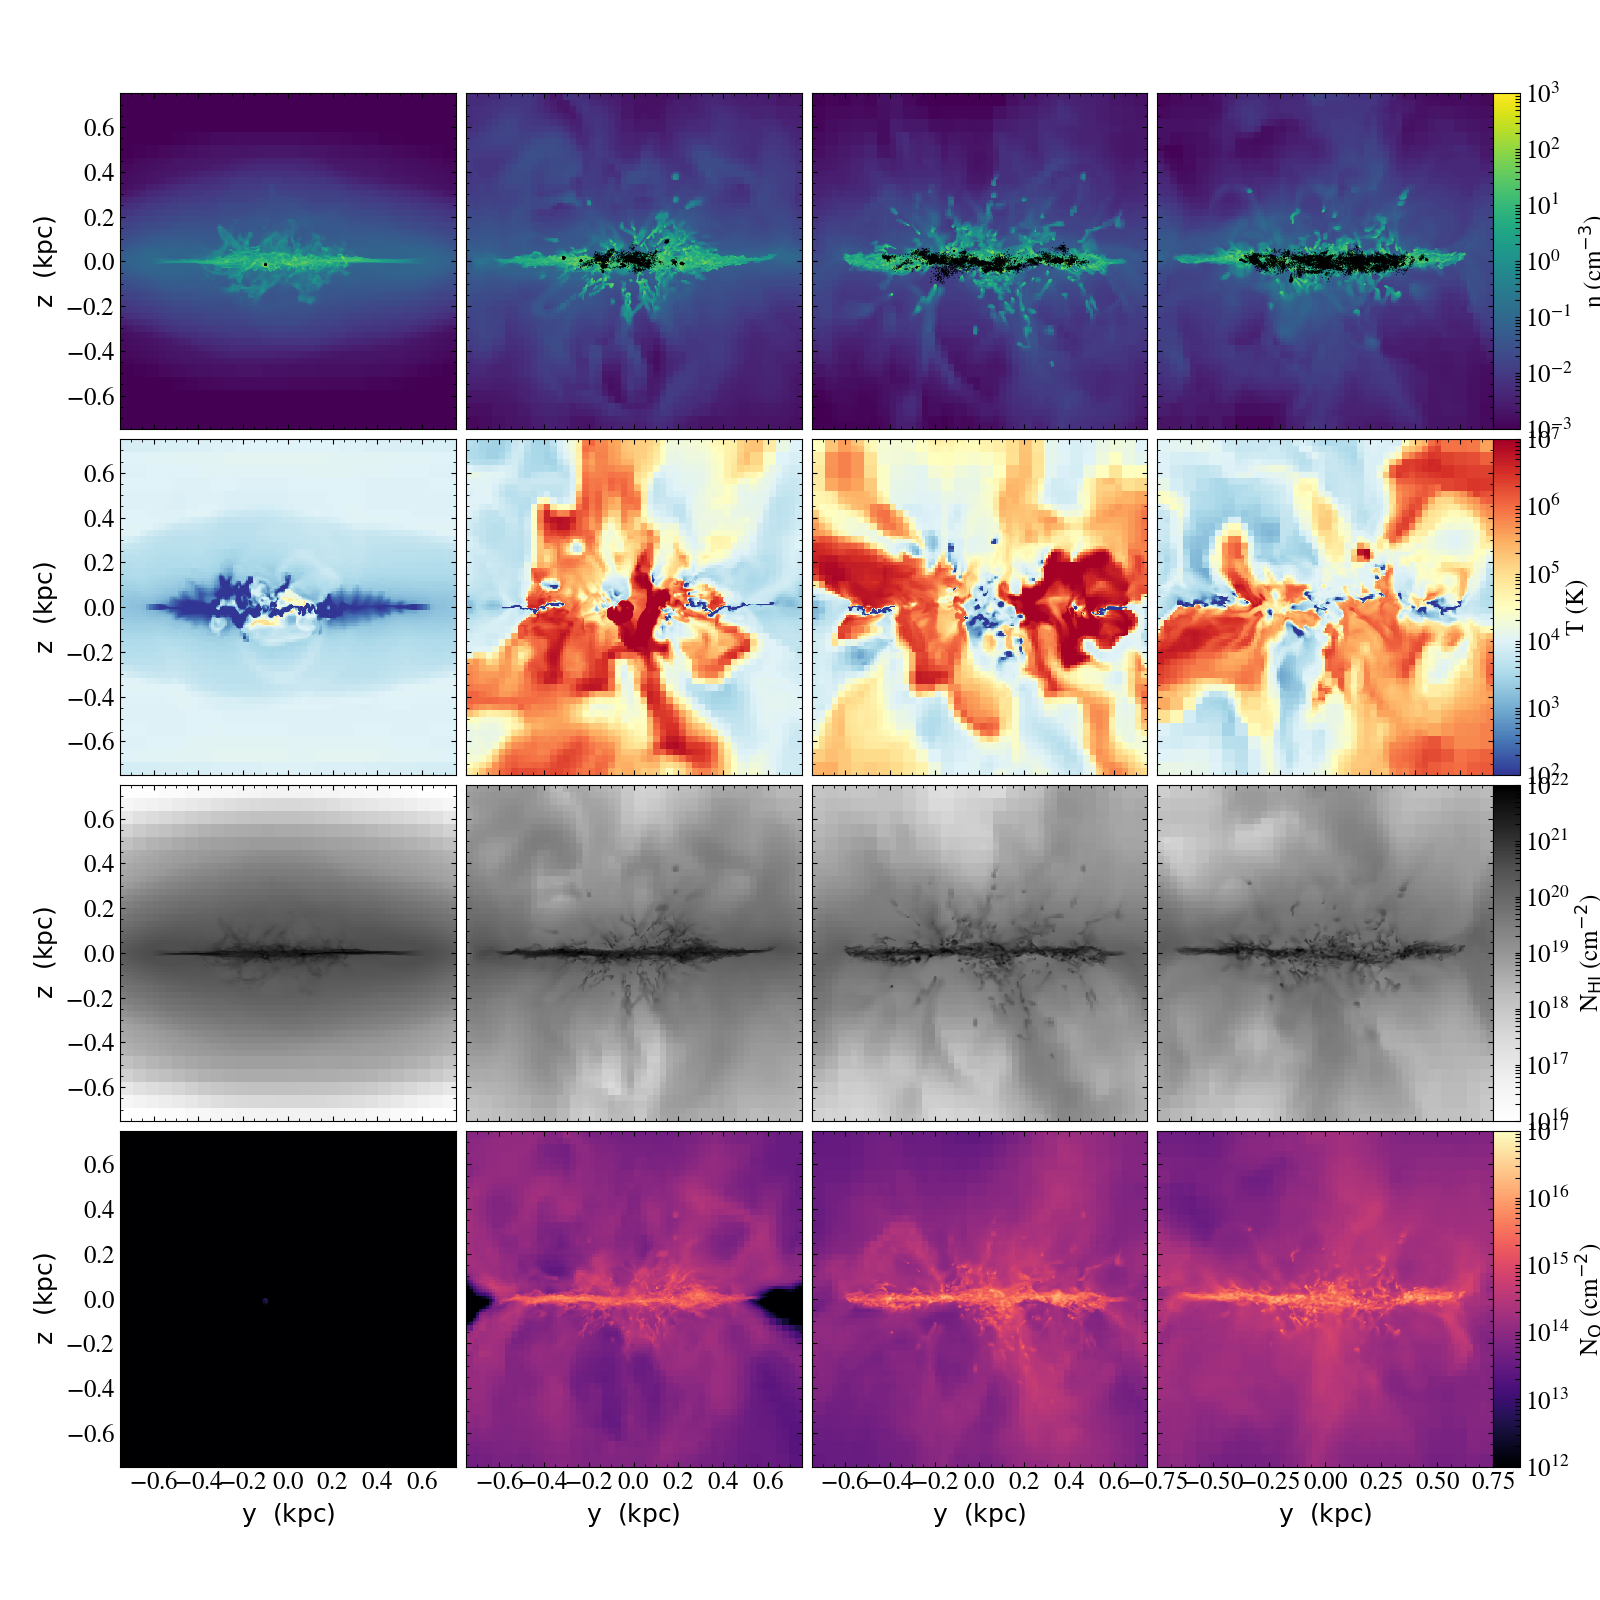
\includegraphics[width=0.975\linewidth]{multiplot_4x4_x.png}
\caption{Edge-on views of our dwarf galaxy at four different times in its evolution, 0, 150, 300, and 500 Myr after the beginning of star formation. Shown are the density weighted projection of number density (top row), temperature slices (second row), 
%mm2 and integrated projections giving 
\ion{H}{1} column density (third row), and H$_2$ column density (fourth row). Each individual main sequence star particle is shown in the number density projections as a single black dot.}
\label{fig:panel_x}
\end{figure*}

The initially puffy gas distribution collapses to a thin disk, with scale heights between 10--30~pc, as shown by the blue line in Fig~\ref{fig:scale_height}. This figure shows the scale height of all gas in the disk, averaged over 40~Myr periods centered on each given time. Stellar feedback acts to heat up this initially thin disk substantially, creating typical scale heights of 50--200~pc. 
%mm2 [moved from above]
  Towards the end of the simulation time, the half-light radius is $390 \pm 21$ pc, where the 
  uncertainty represents the 1$\sigma$ variation in this quantity during the final 20 Myr.
Although the disk remains thin beyond the half-light radius, with a scale height of around 40--60~pc, it is fully resolved at all radii. By the end of the simulation, the majority of the gas has a scale height of $\sim$100~pc. 

Constraining the gas scale height in ultra-faint dwarf galaxies observationally is challenging. For Leo P, located at 1.7~Mpc, \ion{H}{1} observations that are capable of detecting the diffuse \ion{H}{1} throughout the galaxy have a resolution of 100--200 pc, with higher resolution observations identifying only the densest \ion{H}{1} clumps in the galaxy \citep[e.g.][]{Bernstein-Cooper2014}.
%We additionally compute the mass weighted height of the disk, defined as $H = (\sum{Mz^2}/\sum{M})^{1/2}$, where the summation is over each gas cell, as a function of radius (not shown here). $H$ is generally larger than the scale height by a factor of 2, but is comparable to the scale height at radii with ongoing star formation, indicating a particularly uniform-then-truncated density distribution. At large radii, away from active star formation, $H$ is roughly 50 pc, or $\sim$ 3 times the scale height.

\begin{figure*}
\centering
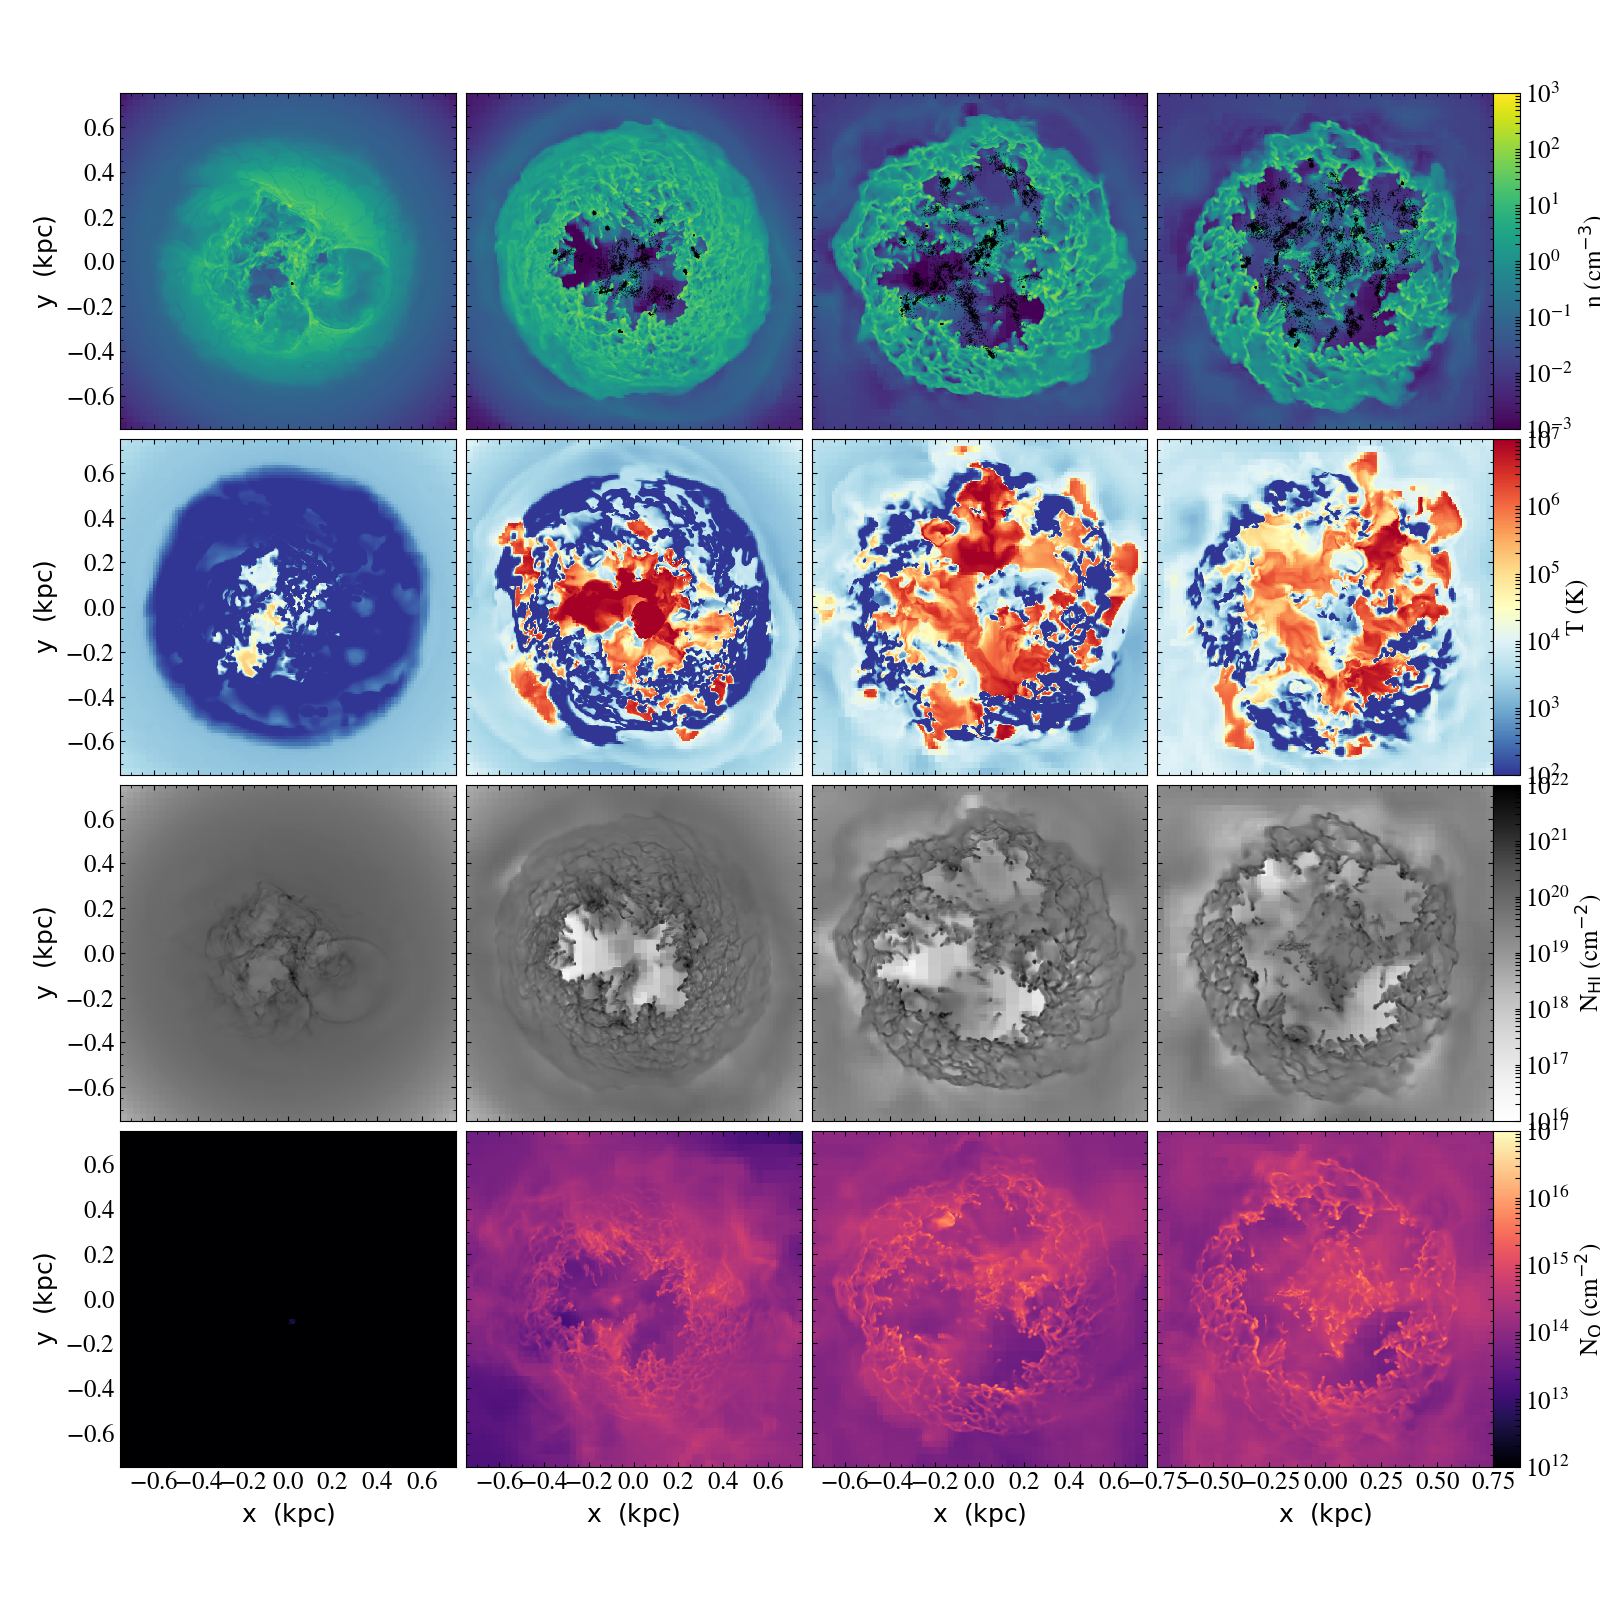
\includegraphics[width=0.975\linewidth]{multiplot_4x4_z.png}
\caption{Same as Figure~\ref{fig:panel_x}, but showing face-on views.}
\label{fig:panel_z}
\end{figure*}

Interestingly, there is significant structure well above the gas disk in our model, in the form of dense clouds and filamentary features, as seen in the edge-on projections. These cold gas clumps appear to have typical sizes on order of $\sim 10$~pc, but with lower density tails that can extend up to 100 pc. These consist of both cool, self-gravitating gas clumps that are being pushed out and ablated by the stellar feedback driven winds, and gas that is cooling and condensing in the disk-halo interface of our dwarf galaxy. These clumps have typical velocities on order of a few to tens of kilometers per second, and appear to survive for 10--100 Myr before being fully ablated or re-accreted onto the main body of the gaseous disk. The evolution of these dense clumps in the context of the disk-halo interface in our low mass dwarf galaxy will be examined in a future work. 
% AE (left out): This is exciting given recent \citep[e.g.][]{Zheng2017} and ongoing \citep{Zheng2017HST} observational observational work examining the disk-halo interface in nearby galaxies.

\begin{figure}
\centering
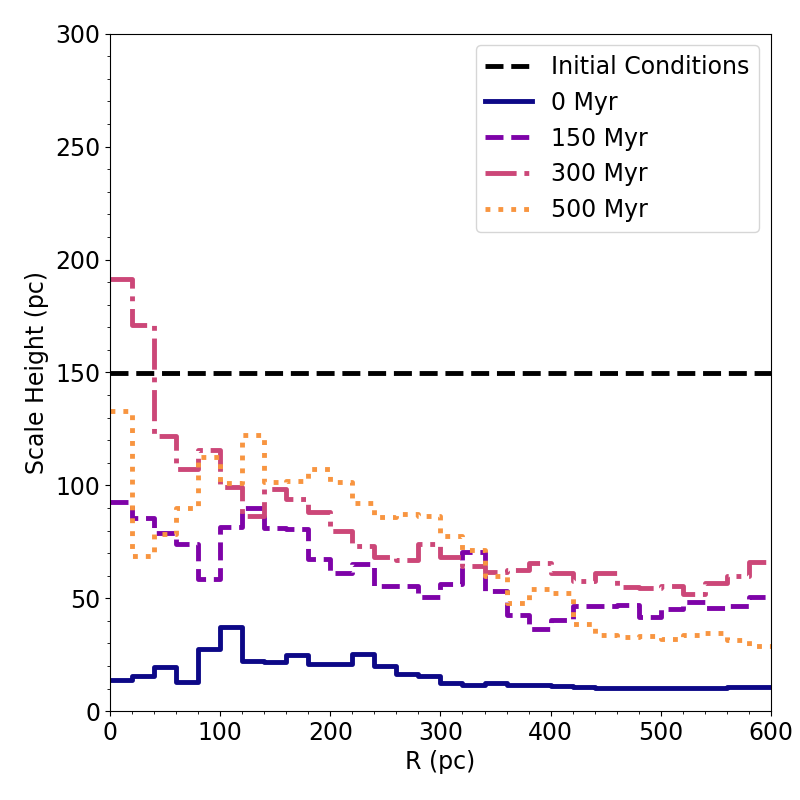
\includegraphics[width=0.975\linewidth]{scale_height}
\caption{The total gas scale height at various times throughout the simulation. These times match the images in Figures~\ref{fig:panel_x} and ~\ref{fig:panel_z}.}
\label{fig:scale_height}
\end{figure}

\subsection{Star Formation Rate and Mass Evolution}
\label{sec:sfr}

We present the star formation rate (SFR) and core collapse supernova rate evolution of our dwarf galaxy as measured in 10 Myr bins in the left panel of Figure~\ref{fig:sfr_mass_evolution}.\footnote{We do not show the Type Ia rate as there have only been 18 by the end of the simulation.} Within the first 40 Myr of evolution the SFR rises quickly to between 2--4$ \times 10^{-4}$ M$_{\odot}$ yr$^{-1}$, remains roughly at this level for 100 Myr, and then drops to an average of about
%mm2
  {\bf [Shouldn't this be $4 \times 10^{-5}$?]}
 $4 \times 10^{-4}$ M$_{\odot}$ yr$^{-1}$, with large fluctuations. By the end of the simulation, the SFR is very low and 
%mm2
   star formation events are
infrequent, with an average SFR over the final 200~Myr of 2.58$\times 10^{-5}$~M$_{\odot}$~yr$^{-1}$. The SNR tracks the SFR with a time delay, with roughly one core collapse supernovae per 100 M$_{\odot}$ of star formation. Averaging over the entire simulation time, we obtain  $<\rm{SFR}> = 9.93 \times 10^{-5}$ M$_{\odot}$ yr$^{-1}$. We discuss how the SFR of this galaxy compares to observed galaxies in Section~\ref{sec:observation}.

%mm \footnote{  [This is rather too long for a footnote, I think.]
We note that the granularity in our star formation algorithm creates a lower limit to the SFR that depends on the period $\Delta t$ over which the SFR is measured. Since we produce stars in $\sim 100$~M$_{\odot}$ sets, the smallest value for our measured SFR is $\sim 100/ \Delta t$. For $\Delta t = 10$ Myr this is 10$^{-5}$ yr$^{-1}$. Removing the granularity requires a fundamental change in our star formation algorithm, likely at the cost of increased complexity and computational expense. Sink particles, which track pre-main sequence stellar mass accumulation, would be the most viable way to do this \citep[see for example ][]{Krumholz2004,Federrath2010,GongOstriker2013,BleulerTeyssier2014,Sormani2017}.

At initialization, all H and He of our dwarf galaxy is neutral, with no molecular hydrogen component. By the time of first star formation ($t=0$ in Figure~\ref{fig:sfr_mass_evolution}), \ion{H}{1} still dominates the mass of the galaxy, but a fairly significant component of molecular hydrogen has formed, with a mass of about $6 \times 10^5$ M$_{\odot}$, or roughly 17\%, of the total mass in the galaxy's disk. The total amount of molecular hydrogen mass in the system remains fairly consistent throughout the evolution, yet its fraction increases over time to roughly 35-40\% and is about equal with the \ion{H}{1} gas. This is because the total amount of mass in the disk decreases through feedback-driven winds, but the H$_2$ is preferentially retained. Small fluctuations in the H$_2$ mass correspond with small increases in the total stellar mass, as some small fraction of H$_2$ is converted into stars, and more is destroyed from the subsequent feedback. Examining the molecular properties of the ISM in low mass dwarf galaxies in more detail is a vital avenue of future research, as there are significant observational uncertainties in deriving H$_2$ content of galaxies in this low metallicity regime \citep{Leroy2008,McQuinn2012,Amorin2016}. The molecular properties of our galaxy are discussed further in context with other works in Section~\ref{sec:observation}. 

\begin{figure*}
\centering
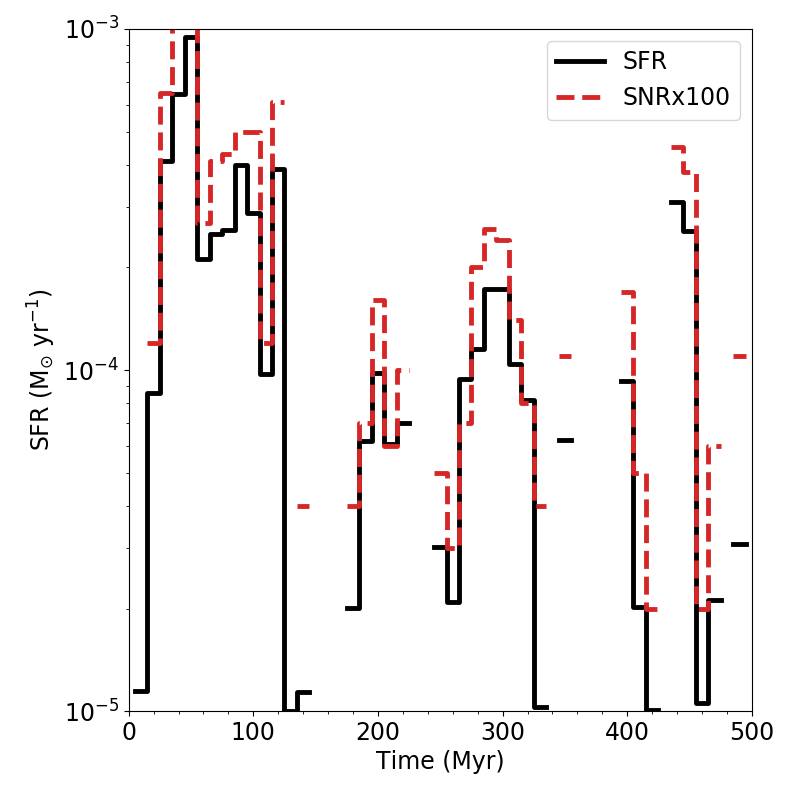
\includegraphics[width=0.475\linewidth]{sfr_snrx100}
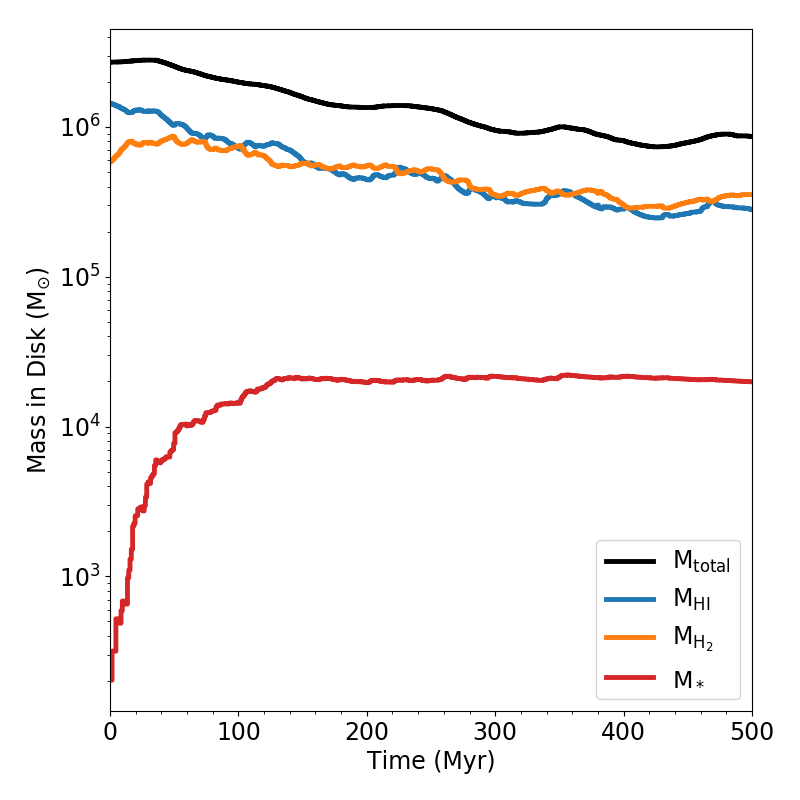
\includegraphics[width=0.475\linewidth]{mass_evolution}
\caption{Left: The SFR and core collapse supernova rate in our dwarf galaxy in 10 Myr bins (left). Right: The evolution of the total gas mass (black), \ion{H}{1} mass (blue), H$_2$ mass (orange), and stellar mass (red) in the disk of our galaxy over time. 
%mm2 Note that the vertical axis limits in the left panel have been scaled to the same numerical values, yet with different units for the SFR and supernova rate.
   Note that the supernova rate has been scaled by a factor of 100 to fit on the same vertical 
   axis as the SFR.}
% This figure only includes gas present within the disk of the galaxy, as defined in the beginning of ~\Section{sec:results}.
\label{fig:sfr_mass_evolution}
\end{figure*}

%mm2 \subsection{Phase Diagrams and ISM Properties}
\subsection{ISM Properties}

\label{sec:phase}

Our simulations include sufficient resolution and microphysics to capture a multi-phase medium within the ISM and halo of our simulated galaxy. We define five different gas phases following those defined in \citep{Draine2011}: molecular gas, cold neutral medium (CNM), warm neutral medium (WNM), warm ionized medium (WIM), and hot ionized medium (HIM). We emphasize that the molecular ISM phase is defined as all regions with f$_{\rm H_2} > 0.5$, and is thus somewhat different than simply considering the total H$_2$ content as decoupled from the rest of the gas. See Appendix \ref{appendix:phases} for a quantitative definition of these phases. Each of these phases exist throughout our simulation, and are regulated by the complex interplay between cooling, turbulence, self-gravity, and 
%mm2 diffuse 
  radiative
and shock heating from stellar feedback throughout the galaxy's evolution. Here we discuss the %mm phase
   thermodynamic 
properties of the gas within the inner halo of our dwarf galaxy.

Figure~\ref{fig:phase} shows the temperature-density 
%mm2 phase diagram 
    distribution
of all gas within 0.25 R$_{\rm vir}$ of the center of the galaxy, averaged over the time period 300--350~Myr. One can readily identify the two
%mm2  most massive regions of gas [eliminated phase language below for consistency with your claim a bit further down the para that there are not well-defined phases.]
    regimes containing most of the mass 
in the simulation: low density, warm gas produced through ionization and supernova heating, and cold, high density gas that makes up most of the mass in the galaxy's disk (see Figure~\ref{fig:ISM_evolution}). Several notable features of the 
%mm2 phase diagram 
     distribution
include: broad ranges of temperature even in quite dense gas, perhaps produced by photoionization and photoelectric heating, a substantial amount of extremely cold gas below 10~K, and the lack of well-defined thermal phases due to the complexity of both the heating and cooling in a turbulent medium. We note that we are likely missing important physics, such as cosmic ray heating and ionization, that would prevent the formation of the coldest gas in this diagram (below about 10~K), but we do not expect this to significantly alter our results. The boxed regime in the lower right corner shows our star formation density and temperature threshold. Gas in this regime is rapidly consumed by star formation and subsequent feedback. Given the small size of our dwarf galaxy, the total amount of mass in this regime at any given instant can be small, but does show up in this time average. We will investigate the typical formation and destruction timescales of this dense, star forming gas in future work.

\begin{figure}
\centering
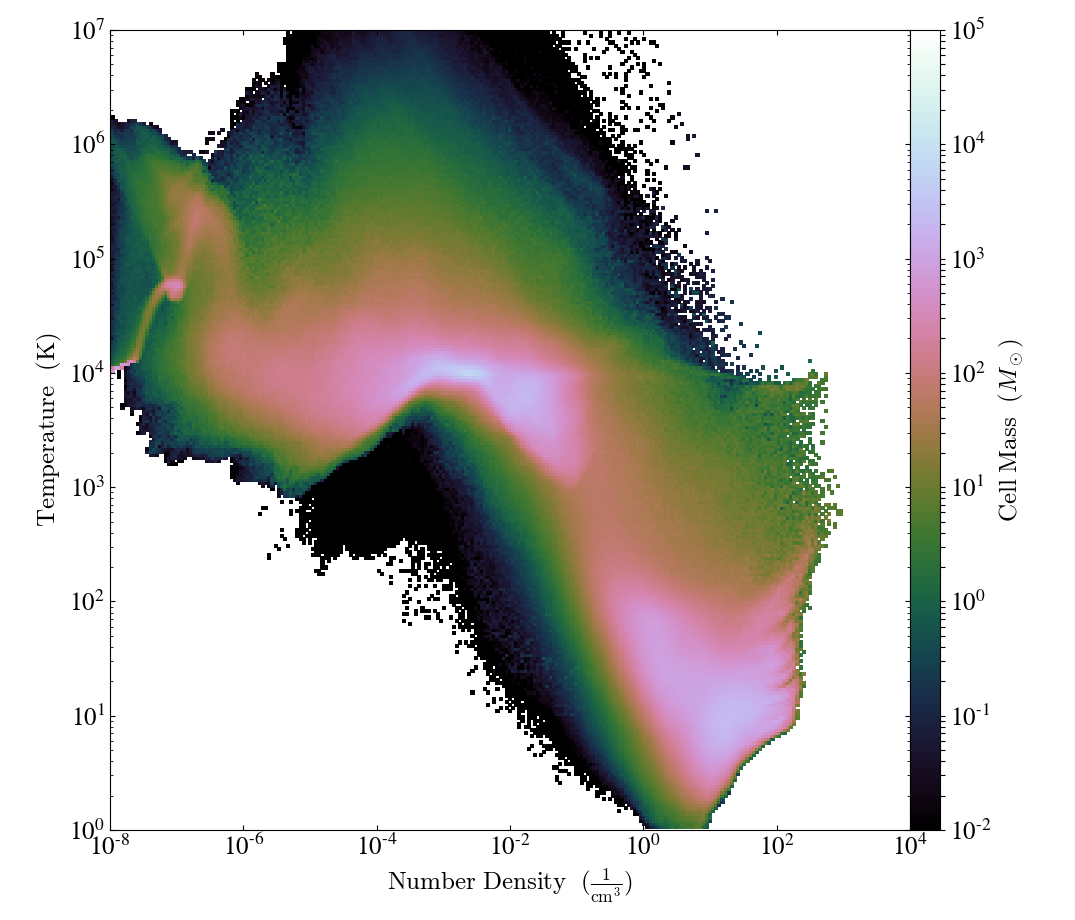
\includegraphics[width=0.95\linewidth]{phase_diagram.png}
\caption{The temperature vs.\ number density phase diagram of our dwarf galaxy simulation showing all gass interior to 0.25~$R_{\rm vir}$, averaged over a 50~Myr period from t~=~300~Myr to t~=~350~Myr. The two red dashed lines show lines of constant pressure for guidance. The region in the lower right corner indicates our density and temperature thresholds for star formation.}
% This figure only includes gas present within the disk of the galaxy, as defined in the beginning of ~\Section{sec:results}.
\label{fig:phase}
\end{figure} 

The mass of the ISM in our dwarf galaxy is dominated by the CNM for the first 200~Myr of simulation time, as shown in the left panel of Figure~\ref{fig:ISM_evolution}. After this point, the molecular component dominates through the end of the simulation.
%mm2 [remove para break]
Together, the CNM and molecular phases comprise $\sim 90\%$ of the total ISM mass, with the remaining mass dominated by the WNM. While the CNM has a negligible volume fraction, the WNM, WIM, and HIM each occupy roughly the same volume fraction. However, the frequent fluctuations in the HIM volume fraction mean that the WIM and WNM more consistently dominate the volume of the galaxy. Together, these figures better quantify the general properties observed in the panel plots in Figure~\ref{fig:panel_x} and Figure~\ref{fig:panel_z}. 

%mm[new para]
These results are in contrast with those found for the more massive dwarf galaxy in \citet{Hu2016,Hu2017}. They find the mass and volume fraction of the ISM nearly entirely dominated by warm gas (ionized and neutral), with cold gas having $\sim$ 10\% of the mass, and occupying negligible volume, and hot gas occupying $\sim$ 10\% of the volume, but having negligible mass. Our lower mass, lower metallicity galaxy contains more cold gas (by mass fraction) by a large factor, and more hot gas (by volume fraction) by a factor of a few. The driver of these differences, which are likely somewhat related to differences in the dark matter halo potential, will be investigated in future work.

\begin{figure*}
\centering
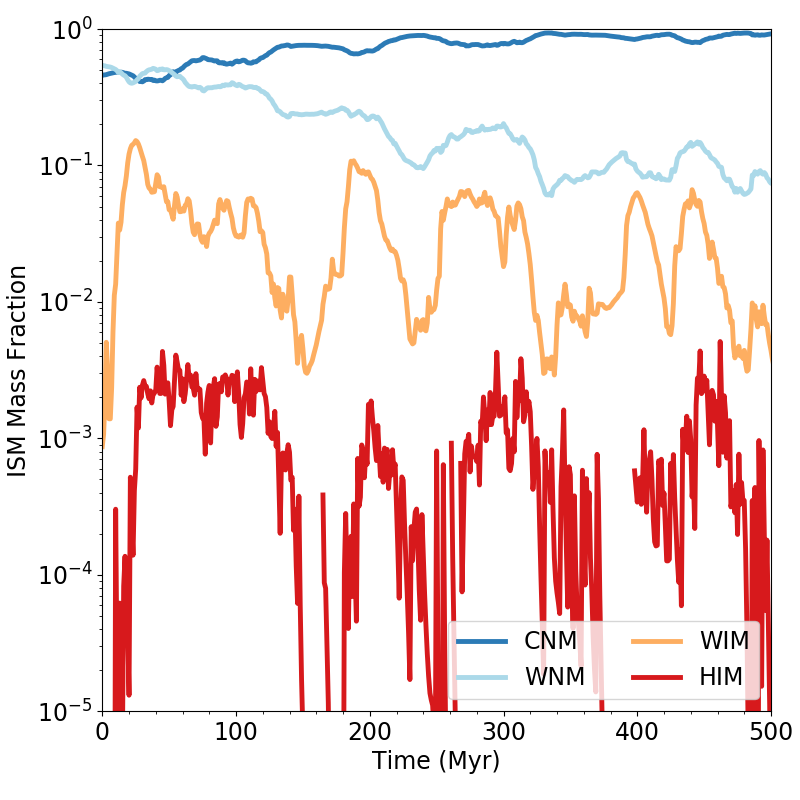
\includegraphics[width=0.45\linewidth]{phase_mass_fraction_evolution_log.png}
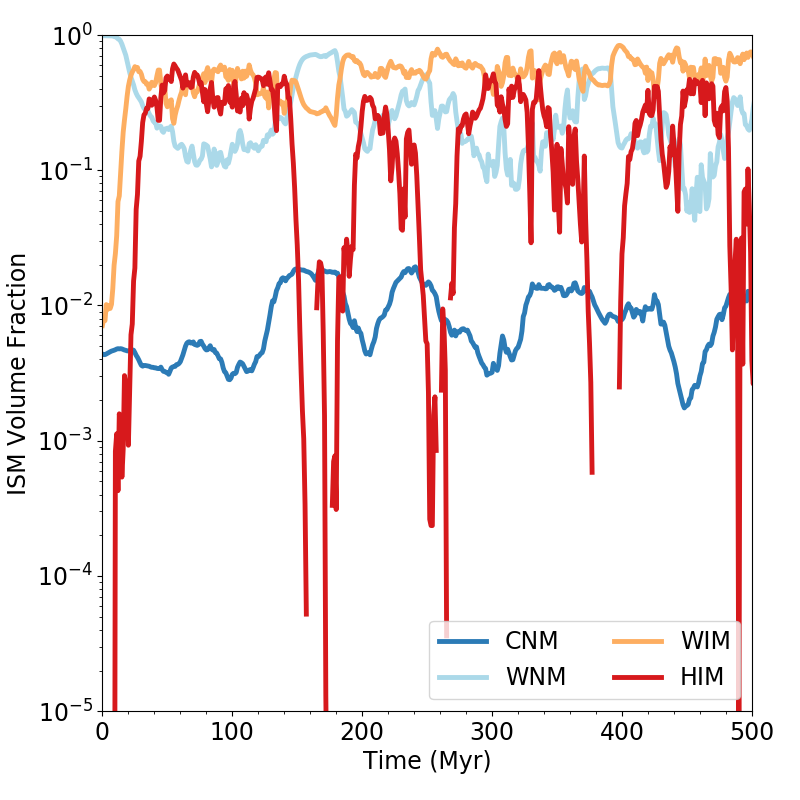
\includegraphics[width=0.45\linewidth]{phase_volume_fraction_evolution_log.png}
\caption{The evolution of the mass and volume fractions for each phase of the model galaxy's ISM.}
% This figure only includes gas present within the disk of the galaxy, as defined in the beginning of ~\Section{sec:results}.
\label{fig:ISM_evolution}
\end{figure*}

\subsection{Interstellar Radiation Field}
\label{sec:ISRF}

The interstellar radiation field (ISRF) of our galaxy varies dramatically in both space and time, as has been seen previously in works modeling varying radiation fields both as expected from stellar motions in our own galaxy \citep{Parravano2003}, and in models including radiation \citep[e.g.][]{Hu2017}. This is not particularly surprising in our low SFR regime, where there can be large fluctuations over time as individual massive stars form, move about, and evolve. In Figure~\ref{fig:ISRF} we present azimuthally averaged radial profiles of the ISRF in various bands, time averaged over 50 Myr from 300--350~Myr. The top panel shows $G_{\rm o}$, the ISRF flux between 6--13.6~eV normalized to the value in the solar neighborhood of the Milky Way (see Sec.~\ref{sec:diffusive heating}). The contribution from the metagalactic background falls below the lower vertical axis limit on this plot. Interestingly, the averaged profile appears nearly flat for most of the disk, with an increase at higher radii due to more recently formed stars. However, the ISRF varies significantly over time, fluctuating by an order of magnitude or more at any given radius. 

\textbf{In response to MM's comment: I focus on G$_o$ here because I found it to be the more general quantity, getting at how one should think of / model the time-and-space-varying ISFR in a tiny dwarf galaxy (i.e. how does this compare to a uniform or 1D radial profile). G$_{eff}$ is convolved with local density and temperature variations, and is thus a bit harder to parse / interpret. Though possibly I should show both?}

\begin{figure}
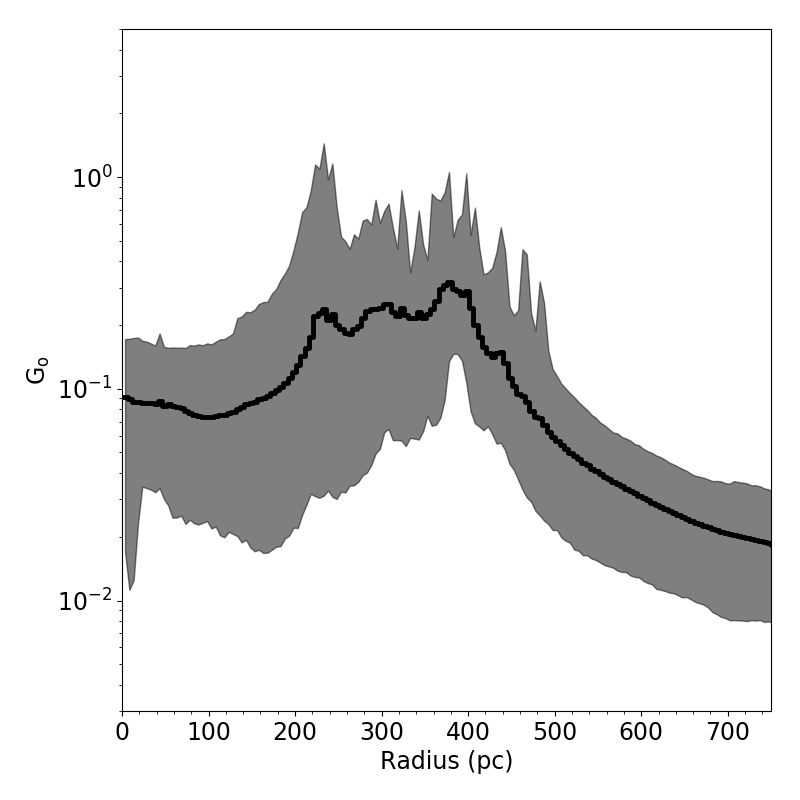
\includegraphics[width=0.95\linewidth]{G_o_profile} \\
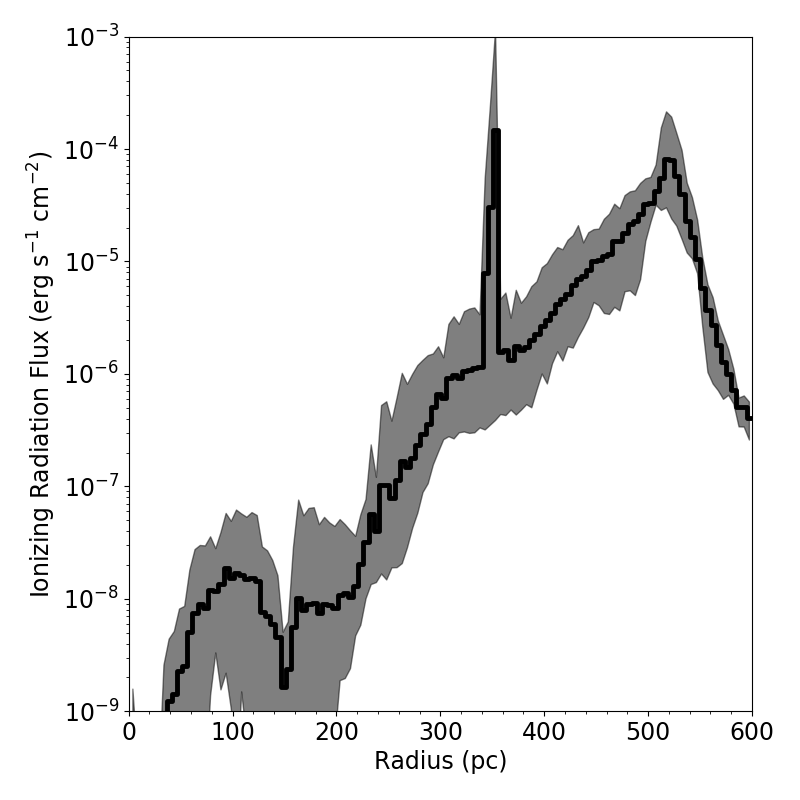
\includegraphics[width=0.95\linewidth]{ionizing_photon_profile}
\caption{
Azimuthally averaged radial profiles of the ISRF in the mid-plane of our galaxy in two different bands, time-averaged over 50 Myr from 300 -- 350~Myr. Here we define the midplane as within 2.5~$dx$ of z = 0, or 4.5~pc. The top panel gives $G_{\rm o}$, the flux of radiation between 6--13.6 eV normalized to the value in the solar neighborhood, shaded between minimum and maximum values at each position, with the average shown as a black line. The bottom panel gives the \ion{H}{1} ionizing stellar radiation flux. Since this radiation is tracked directly through radiative transfer, the minimum value at all radii is 0 at some point. For this reason we only shade between the first quartile and maximum values. \ion{He}{1} is very similar to \ion{H}{1}, with a small vertical offset, and is not shown for clarity.}
\label{fig:ISRF}
\end{figure}

The bottom panel gives the ionizing photon fluxes for \ion{H}{1} from stellar radiation {\em only}. Since this field is tracked directly using ray-tracing radiative transfer, the profile encodes information about local attenuation of these photons from dense, neutral gas. This is the main driver of the differences between this field and $G_{\rm o}$. However, both profiles track each other well as a function of radius. The lack of dramatic trend with radius in both diagrams suggests that one could model the ISRF in low mass dwarf galaxies using a uniform heating / ionization rate; however, this would still fail to capture the fact that any given region of the galaxy will experience order of magnitude or more fluctuations in the incident flux. 
% These fluctuations are likely important in reducing star formation locally around young, massive stars. This effect would be challenging to capture with a simple model. (AE this bit is moved to the end of section)

\begin{figure*}
\centering
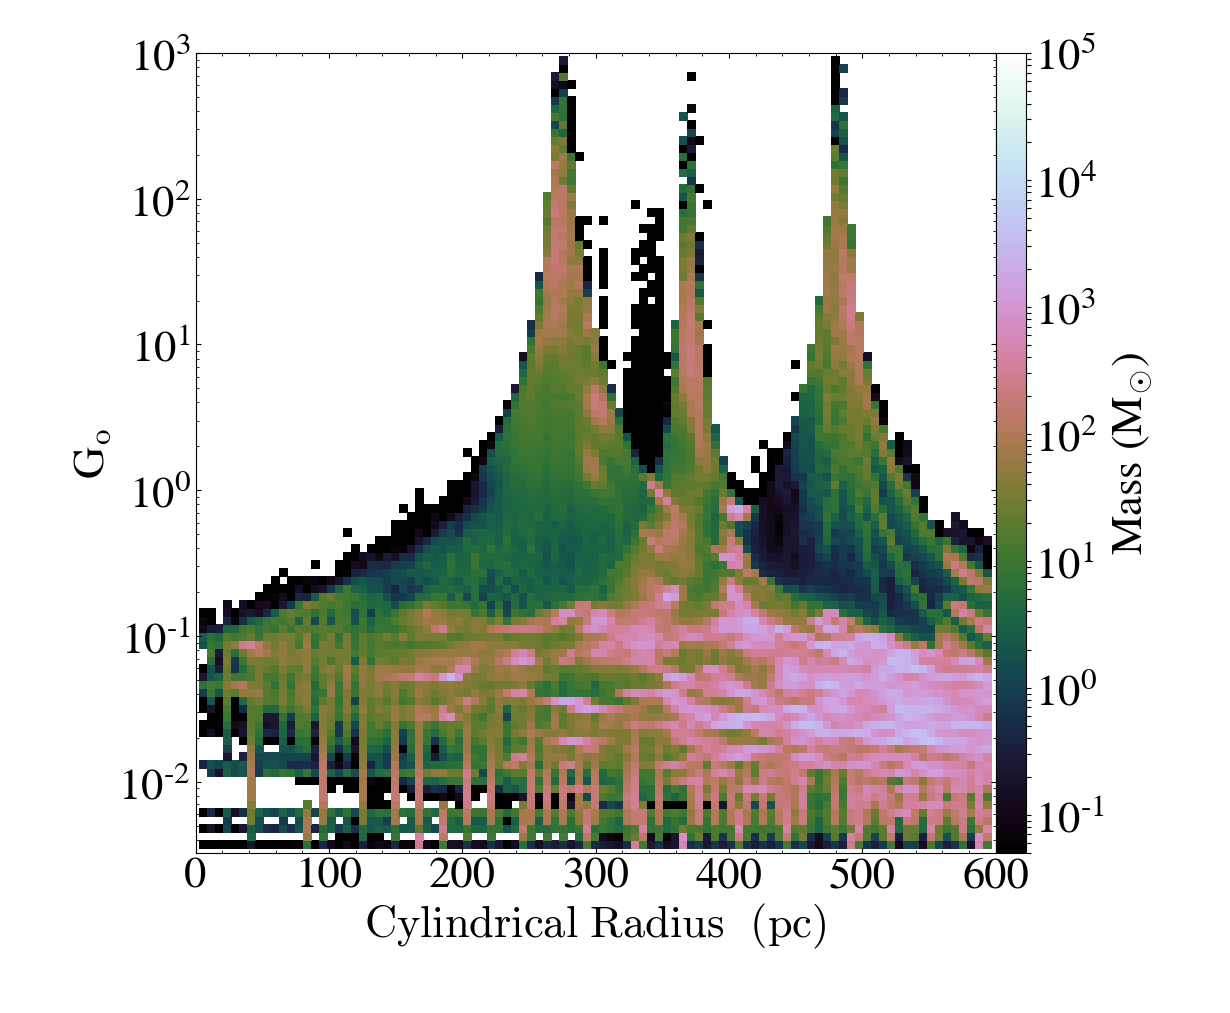
\includegraphics[width=0.45\linewidth]{g_o_2D_phase}
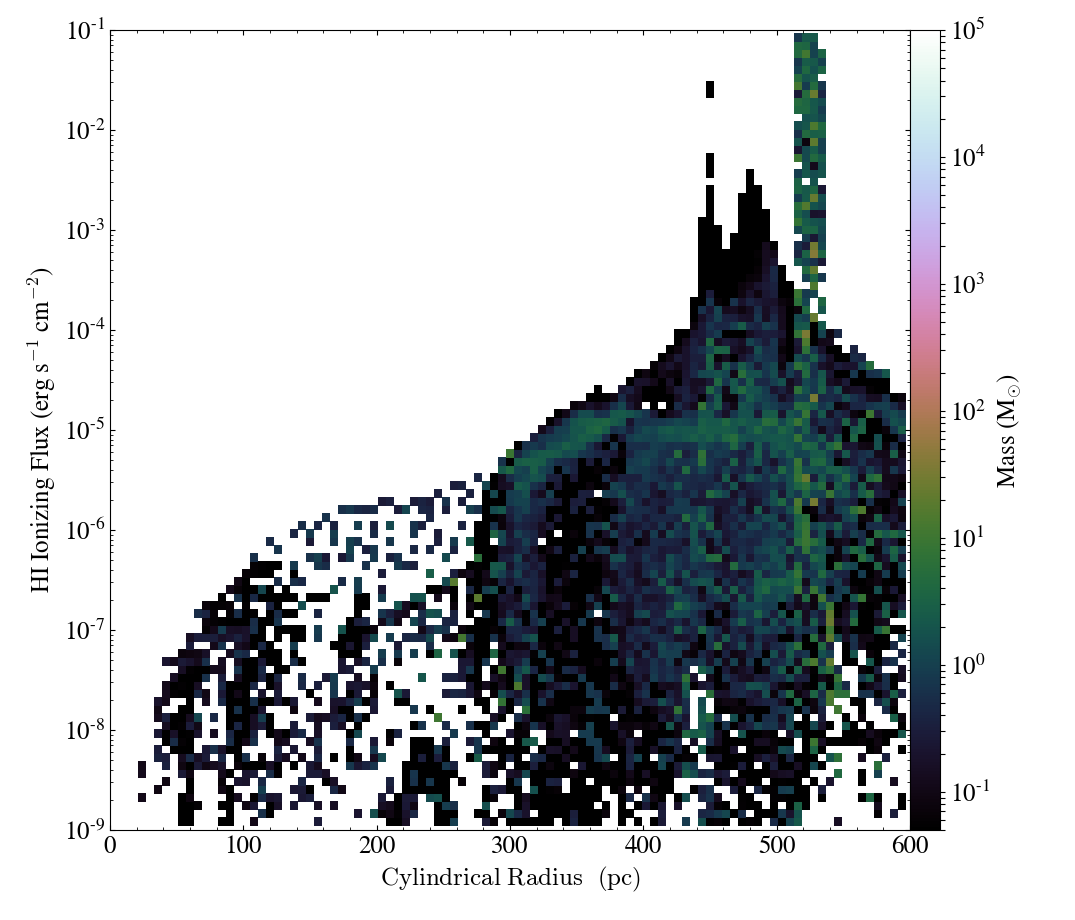
\includegraphics[width=0.45\linewidth]{q_o_2D_phase}
\caption{Single-snapshot 2D radial profile plots at 200~Myr of the ISRF in two flux bands, $G_{\rm o}$ and \ion{H}{1} ionizing radiation, illustrating the full dynamic range of radiation flux at a given radius in the galaxy. Here, we include all gas within the mid-plane of our dwarf galaxy. Since a majority of the mass of the galaxy is in the cold phase (see Figure~\ref{fig:phase}), and is therefore optically thick to \ion{H}{1} ionizing radiation, it does not show up in the \ion{H}{1} ionizing radiation diagram. This gas readily appears in the $G_{\rm o}$ diagram since we assume it to be optically thin, though we do apply a localized shielding approximation.}
\label{fig:ISRF_2D}
\end{figure*}

To further quantify the local variations in these radiation fields, we present the full distribution of $G_{\rm o}$ and the \ion{H}{1} ionizing flux in Figure~\ref{fig:ISRF_2D} at a single snapshot at 200~Myr. This diagram shows how dramatic the increase in ISRF near young, massive stars is (the spikes in both diagrams), while much of the mid-plane sees an ISRF orders of magnitude lower. The striking contrast between the two diagrams is due to the shielding of the \ion{H}{1} ionizing flux in the most massive (cold and dense) regions of the galaxy through the radiative transfer calculations; shielding of the FUV radiation is approximate and in general weaker, making these regions more prominent in the left hand figure (the pink/white clumps). From both of these diagrams, it is clear that the ISRF of a low mass dwarf galaxy various greatly over time and space in a way that cannot be appropriately captured by an analytic profile. Although one could adopt an averaged radial profile to provide a realistic, global source of energy for thermal pressure support of the gas against collapse, it is unclear how sufficient this would be in suppressing star formation. In particular, the large increases around sites of recent star formation could be important sources of feedback to destroy molecular clouds and reduce their effective star formation efficiency. It 
%mm2 is unclear 
   remains to be seen
which of these two modes of feedback is more important in controlling star formation.

%mm (Emerick et. al. in prep).  [I'd only insert the reference when there is an actual astro-ph number to support it.] 

\subsection{Outflow Properties}
\label{sec:outflows}

The recent FIRE cosmological simulations of dwarf galaxies over a range of dark matter halo masses find that they exhibit large outflows, with mass loading factors on order of 100--1000 \citep{Muratov2015}. However, comparable models of idealized dwarf galaxies with detailed feedback and physics treatments find more modest mass loading factors \citep{Hu2016,Hu2017}. In Figure~\ref{fig:mass_outflow} we present the mass outflow and mass loading rates for our dwarf galaxy as a function of time, computed at five different positions from the galaxy. We follow \citet{Muratov2015} in defining the mass outflow rate at any given radius to be the sum of the outflow rate in all cells in a spherical annulus of width $dL$ centered at that radius,
\begin{equation} \label{eq:dotM}
\dot{M}_{\rm out} = \sum M_{\rm gas} \times v_{\rm r} / dL.
\end{equation} 
We choose $dL = 0.1~R_{\rm vir}$, or 2.74 kpc. 

The total mass outflow rates and mass loading factors at 0.1, 0.25, 0.5, and 1.0 $R_{\rm vir}$ are shown in Figure~\ref{fig:mass_outflow}. Generally, other works use gigayear timescale measurements of the SFR to compute the mass loading factor. For consistency with those works, we use the 500~Myr average SFR for computing the mass loading factor. The outflow rate at 0.1 $R_{\rm vir}$ is high, corresponding to mass loading factors on order of 50--100 throughout the simulation time. This quickly declines towards larger radii, however, with minimal outflow past the virial radius. \citet{Muratov2015} finds typical mass loading factors at 0.25 R$_{\rm vir}$ on order of 20--40 for galaxies with $v_{c} = 30$ km s$^{-1}$ at low redshift. Our dwarf galaxy exhibits mass loading factors between 4 and 40 at this radius; this is consistent with the results from \citet{Muratov2015}, but perhaps slightly below their typical values. 

Interestingly, the v$_{\rm c}\sim$ 30 km s$^{-1}$ halos examined in \citet{Muratov2015} are more massive than the M$_{\rm vir} = 2.5\times 10^9$ M$_{\odot}$ halo examined here by a factor of a few. Using a fit provided in \citet{Muratov2015} to extrapolate and compare at fixed halo mass, one would expect mass loading factors on order of 100 at 0.25 R$_{\rm vir}$ for our dwarf galaxy, a factor of a few higher than what we find. These differences could be attributed to our lack of cosmological evolution in these isolated simulations, but ultimately requires a larger set of dwarf galaxy simulations to make a more robust comparison. We note, however, that our results are much closer to the \citep{Muratov2015} results than those in \citet{Hu2016,Hu2017}, which find mass loading factors at 0.05 $R_{\rm vir}$ between 1 and 10 for a dwarf galaxy with M$_{\rm vir} = 10^{10}$ M$_{\odot}$, and therefore certainly have much smaller mass loading factors at 0.25 $R_{\rm vir}$.

% figure here of mass loading and mass outflow rates
\begin{figure*}
\centering
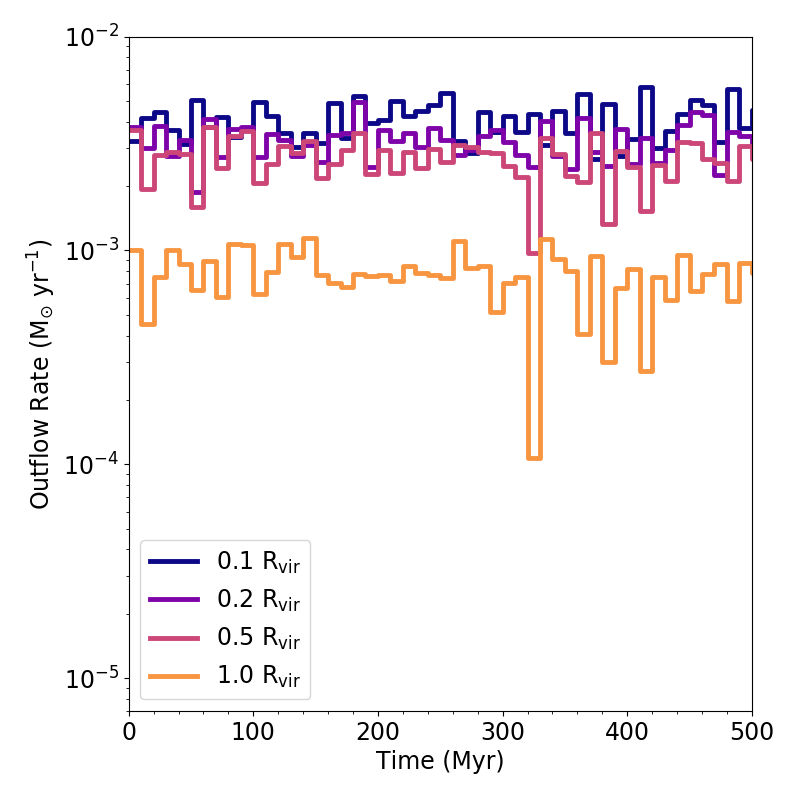
\includegraphics[width=0.45\linewidth]{total_mass_outflow}
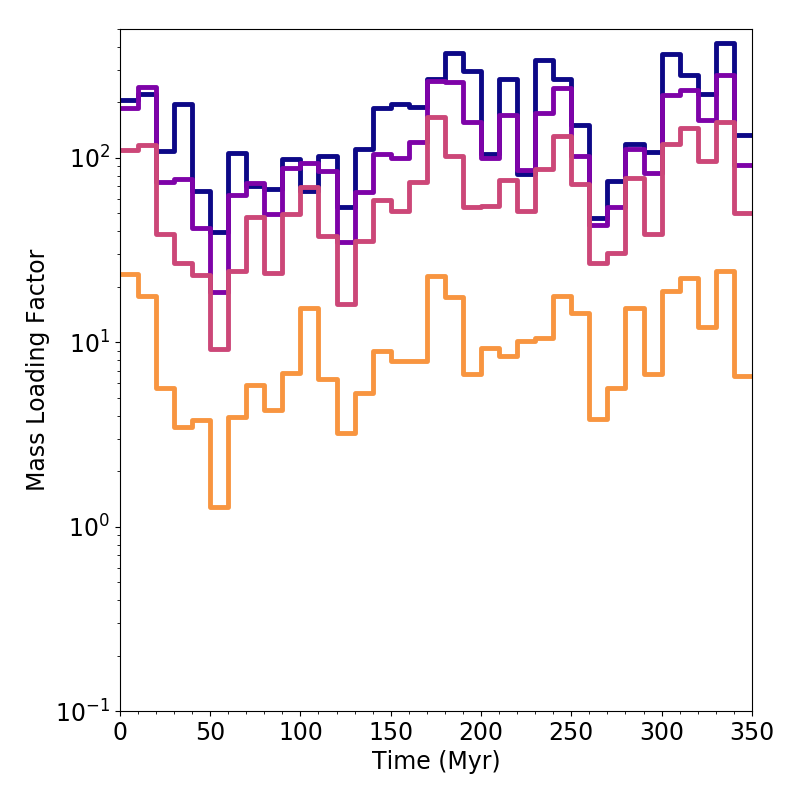
\includegraphics[width=0.45\linewidth]{total_mass_loading}
%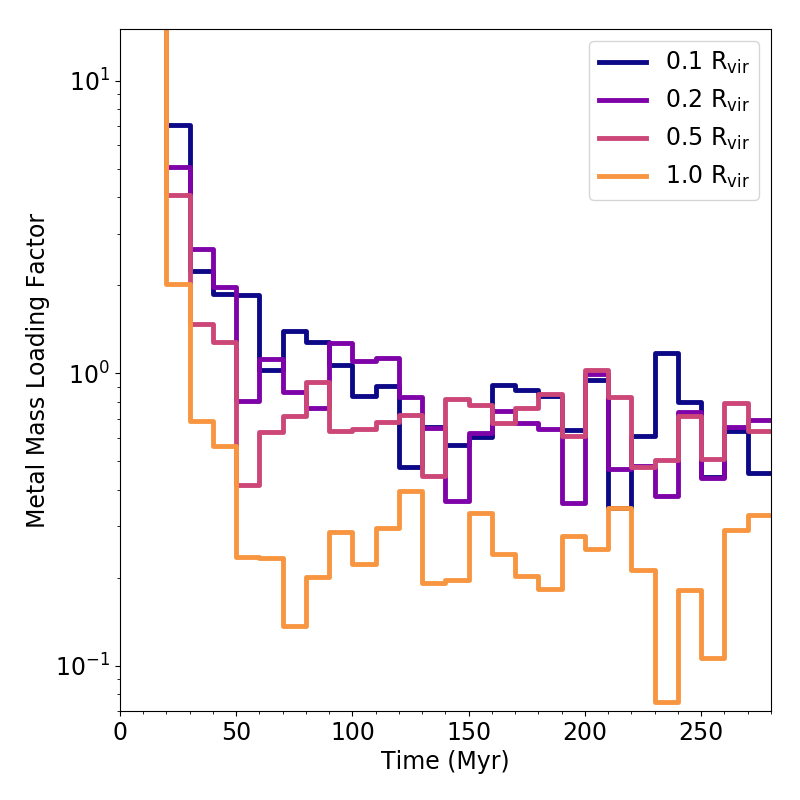
\includegraphics[width=0.33\linewidth]{metal_mass_loading}
\caption{Spherical mass outflow rates (Eq.~[\ref{eq:dotM}]) and mass loading rates over time at 4 different radii from the galaxy.}
\label{fig:mass_outflow}
\end{figure*}

Detailed outflow properties, beyond outflow rates and mass loading factors, can help discriminate between the model dependent feedback physics included in galaxy simulations. In Figure~\ref{fig:outflow_velocity} we present radial velocity distributions of all material outside our dwarf galaxy's disk, and within the halo, broken into three gas phases. Half of the outflow, by mass, is at velocities below 40 km s$^{-1}$, with 75\% at velocities of 70 km s$^{-1}$ or below. This gas is dominated by the two warm gas phases, with the WNM dominating at lower velocities, and the WIM at higher velocities. The distribution has a very long tail out to and beyond 500~km~s$^{-1}$. The dominant launching mechanism in this simulation are supernovae, generating a rapidly moving and volume-filling HIM, consistent with the results in \citet{Hu2016,Hu2017}. However, as shown, the HIM comprises very little of the outflow by mass. Most of the outflowing gas (by mass) comes from the warm phase, pushed out by the high pressure, fast moving HIM. Some of this warm gas certainly originates from adiabatically and radiatively cooled HIM, however. The amount of transfer between phases in the halo of our galaxy will be investigated in future work.

\begin{figure}
\centering
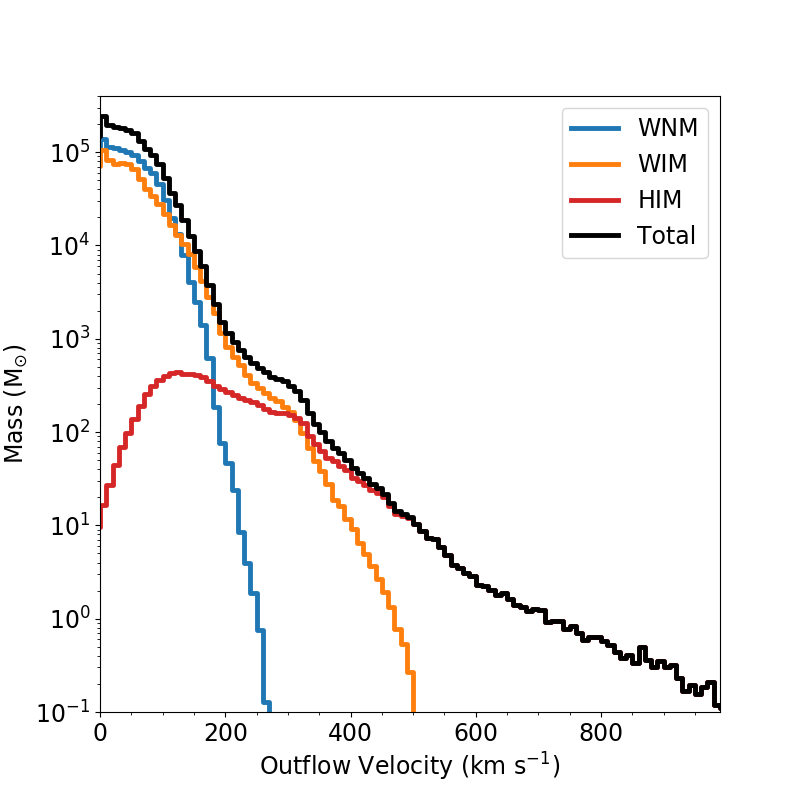
\includegraphics[width=0.95\linewidth]{outflow_velocity_distribution}
\caption{The time averaged radial velocity distribution of outflowing material external to the disk and within the virial radius of our dwarf galaxy. The outflowing material is multiphase, broken into WNM, WIM, and HIM. See Section~\ref{sec:phase} for definitions of these regimes. We note that WNM is often labeled simply as ``cold'', or gas below $T = 10^{4}$K. There is little to no outflowing mass in the CNM or molecular phases.}
\label{fig:outflow_velocity}
\end{figure}

%\textbf{AE: Took plot and discussion of outflow metallicities out and replaced with metal mass loading factor (below)}
%In Figure~\ref{fig:outflow_metallicity} we show the average ISM metallicity (black), halo metallicity (blue), and outflow metallicities (orange) at 0.1 (solid), 0.25 (dashed), and 1.0 (dotted) $R_{\rm vir}$ over the simulation time. The ISM metallicity evolves minimally from the initial conditions in this time, while the halo and outflow properties change significantly. It is apparent from this figure that the outflows are preferentially metal enriched, as the halo increases in metallicity by a factor of $\sim 2$ in the simulation time. Although most of the gas mass in the halo (outside the disk) remains within 0.2 $R_{\rm vir}$ (see Section~\ref{sec:obs_metals}), the mass that does make it to the outer reaches of the halo or beyond is metal enriched by a factor of $\sim$5--6 compared to the ISM. This is in contrast with the results from \citet{Muratov2017}, which generally show $Z_{\rm outflow} \simeq Z_{\rm ISM}$ at $0.25~R_{\rm vir}$ and $Z_{\rm outflow} < Z_{\rm ISM}$ at $1.0~R_{\rm vir}$, though both with some scatter that reaches $Z_{\rm outflow} > Z_{\rm ISM}$, especially at high redshift. However, we note that our simulations certainly do not contain a cosmologically realistic circumgalactic medium, nor do they include ongoing cosmological accretion of pristine gas. Mixing of outflowing, metal enriched gas and pristine inflows will lower the typical halo and outflow metallicities, particularly at large radii.

%\begin{figure}
%\centering
%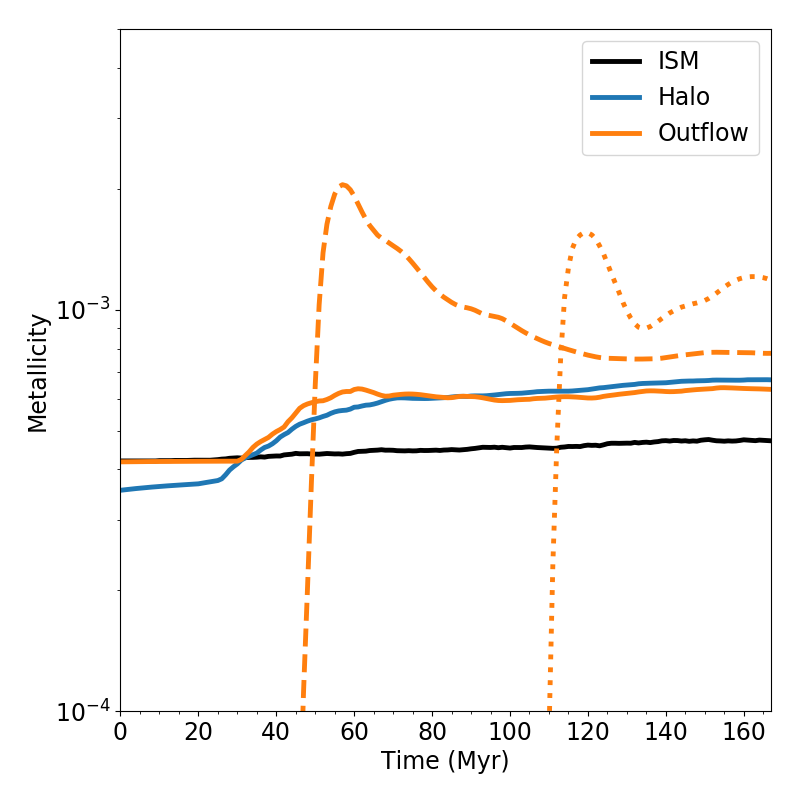
\includegraphics[width=0.95\linewidth]{metallicity_evolution}
%\caption{The mass-weighted average metallicity of our dwarf galaxy's ISM, halo, and outflowing gas at 0.1 (solid), 0.25 (dashed), and 1.0 (dotted) $R_{\rm vir}$ over the simulation time. The halo is defined as the region outside of the disk, yet inside the virial radius.}
%\label{fig:outflow_metallicity}
%\end{figure}

\subsection{Metal Evolution} 
\label{sec:chemical evolution}
%mm2 \textbf{This section saw significant change. Removed previous mention of stellar abundances and species retention fractions. Much of below is new(ish)}

\subsubsection{Metal Enriched Outflows}
Dwarf galaxies efficiently, and preferentially, eject metals released in stellar feedback from their shallow potential wells \citep{MacLowFerrara1999,FerraraTolstoy2000}. This has been better quantified recently both observationally \citep[e.g.][]{Kirby2011-metals,Zahid2012,Peeples2014,McQuinn2015} and with more detailed cosmological simulations \citep{Angles-Alcazar2017,Muratov2017}. In the top panel of Fig.~\ref{fig:metal_evolution}, we give the metal mass loading factor for our galaxy over time, at the same radii as in Fig.~\ref{fig:mass_outflow}. We define the metal mass loading factor as
\begin{equation} \label{eq:eta-metal}
\eta_{\rm metal} = \frac{\dot{M}_{\rm metal}}{\rm{SFR} \times \frac{M_{\rm metal}}{M_{*}}},
\end{equation}
where $\dot{M}_{\rm metal}$ is the metal mass outflow rate, $M_{\rm metal}$ is the total mass in metals produced, and $M_{*}$ is the total mass in stars. We note the very large loading factors in the first 20~Myr are artificial, and a byproduct of the initial conditions. For half of the evolution, the inner three radii give $\eta_{\rm metal}$ below unity (around 0.6), but it increases at each radius, fluctuating around unity for the second half of the simulation. Recent simulations of outflows from a Milky Way type disk indicate typical $\eta_{\rm metal}$ comparable to our results, usually between 0.5 and 1 \citep{Li2017,Fielding2017}. \cite{Muratov2017} computes a slightly different quantity for their galaxies, the normalized metal outflow rate $\eta_{Z} = \dot{M}_{\rm metal}/{\rm SFR}$, finding values of about 0.02 at 0.25~$R_{\rm vir}$ regardless of galaxy circular velocity. Our galaxy is consistent with this value, with an average $\eta_Z = 0.015$, fluctuating between 0.007 and 0.02.

\begin{figure}
\centering
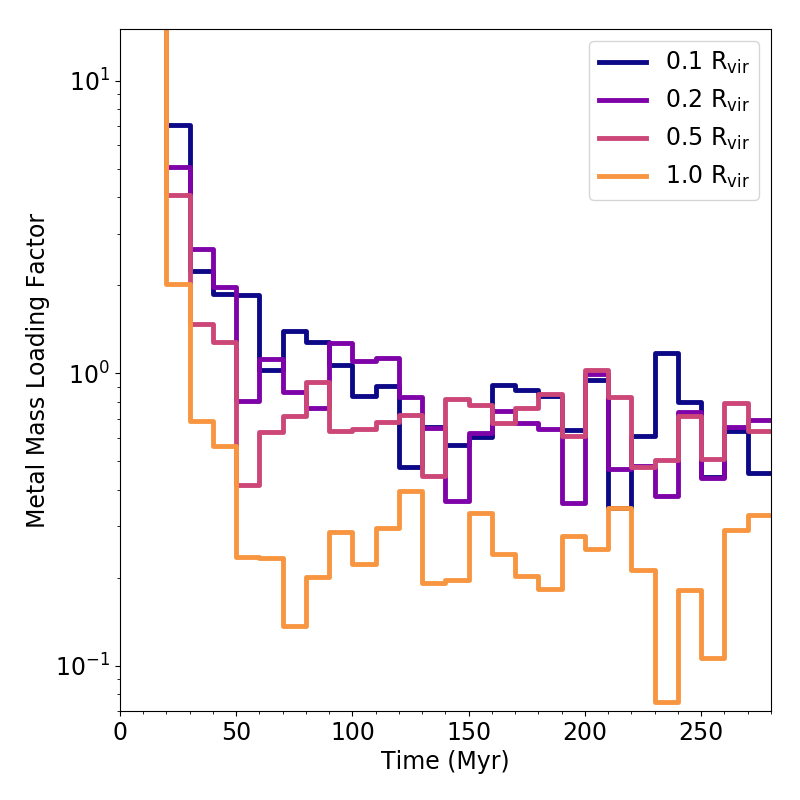
\includegraphics[width=0.9\linewidth]{metal_mass_loading} \\
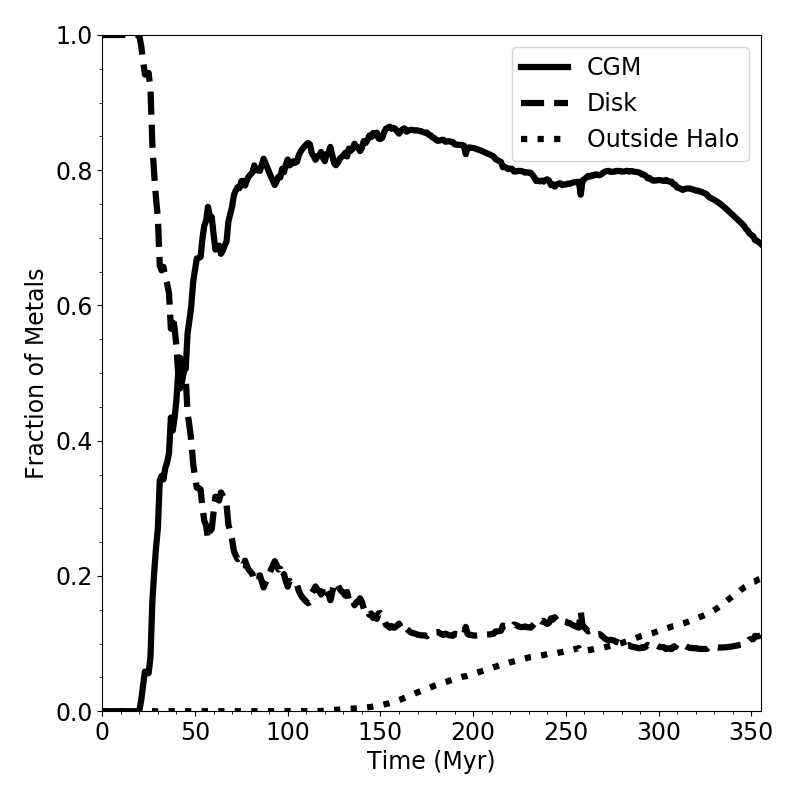
\includegraphics[width=0.9\linewidth]{metal_fraction_evolution}
\caption{Top: Metal mass loading factor (see Eq.~\ref{eq:eta-metal}) at radii of 0.1 ({\em black}), 0.2 ({\em purple}), 0.5 ({\em salmon pink}), and 1.0 $R_{\rm vir}$ ({\em yellow}) over time. Bottom: The fraction of metals contained in the disk, CGM, and outside the halo of our dwarf galaxy over time. In both panels, we consider the total mass of all individually tracked metal species, which is zero at initialization, not the aggregate total metallicity field, which is non-zero at initialization.}
\label{fig:metal_evolution}
\end{figure}

These large metal mass loading factors indicate that a majority of the metals produced in our dwarf galaxy are ejected from the disk. This is quantified in the lower panel of Fig.~\ref{fig:metal_evolution}, where we show the mass fraction of metals in the disk, circumgalactic medium (CGM), and outside the virial radius of our galaxy over time. After the first 20 Myr, supernova-driven winds rapidly drive out large quantities of metals from the disk and into the galaxy's halo. This continues throughout the simulation, with only $\sim$12\% of produced metals residing in the disk of the galaxy. It only takes 150 Myr for some metals to reach the virial radius of the halo, with a steadily increasing fraction continually leaving the virial radius, reaching 40\% by the end of the simulation. Likewise, the CGM metal content continually decreases until the end of the simulation, from loss through the virial radius of the halo. Although the metal content of the ISM gradually decreases throughout the simulation, it seems somewhat steady at $\sim 10\%$ through the final 200~Myr of evolution. See Section~\ref{sec:obs_metals} for further discussion.
%\textbf{closing sentence}

\subsubsection{Metal Distribution within the ISM}

It is important to understand how metals from each source of stellar yields (massive and AGB stellar winds and supernovae) enrich the ISM. Observations of more massive dwarf galaxies than those simulated here indicate fairly uniform radial gas-phase metallicity profiles, even beyond the stellar radius \citep[e.g.][]{Werk2011,Belfiore2017}. This requires that metal mixing and transport occur on hundred megayear timescales, much more rapidly than the gigayear timescale expected from assuming transport at the cold gas sound speed. This suggests either that metals are transported first through a hot phase 
%mm2 
   with high sound speed, 
or by efficient turbulent mixing within the ISM \citep[e.g.][]{Tassis2008,YangKrumholz2012}. It remains uncertain how metal abundances vary in detail within these galaxies, beyond one-dimensional radial profiles, and whether or not abundance distributions depend on the metal species. It is even more unclear how metals are transported and distributed within ultrafaint dwarf galaxies, which generally host too few HII regions for a detailed examination.

We demonstrate the power of our simulations, which capture a realistic ISM at high resolution with multiple feedback sources, by addressing these questions in Fig~\ref{fig:metal_slices}. The top two panels give the slices of number density (top left) and temperature (top right) in the mid-plane of a portion of our dwarf galaxy. These serve to guide the eye in the lower panels, clearly indicating regions with dense, cold gas clouds ($n \sim 100~\rm{cm}^{-2}$, $T \lesssim 100~$K), warm, diffuse gas ($n\sim 0.1$~cm$^{-3}$, $T\sim 10^{4}$~K), and hot gas from a recent SN explosion ($T\sim10^{6}$~K). The bottom panels give abundance ratios for oxygen and hydrogen (bottom left), nitrogen and hydrogen (bottom middle), and nitrogen and oxygen (bottom right). 

\begin{figure*}
\centering
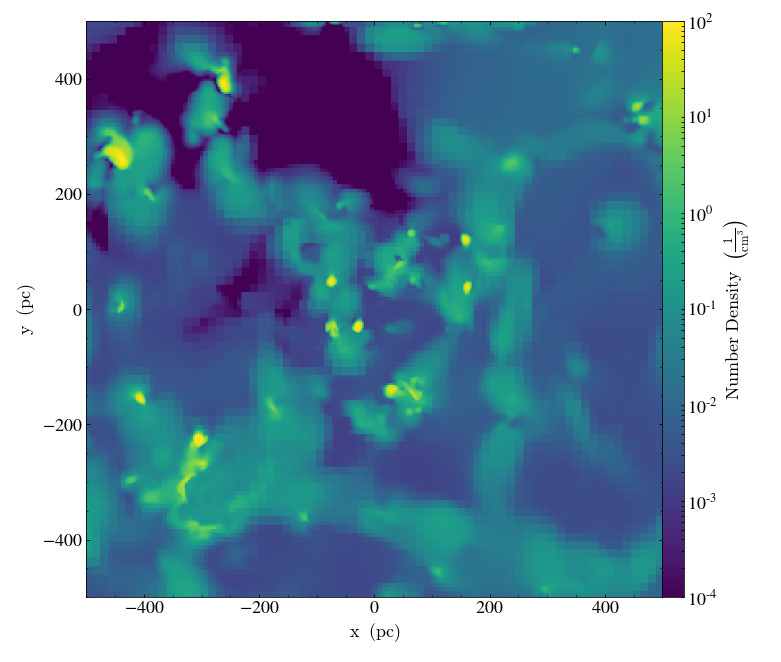
\includegraphics[width=0.32\linewidth]{number_density} 
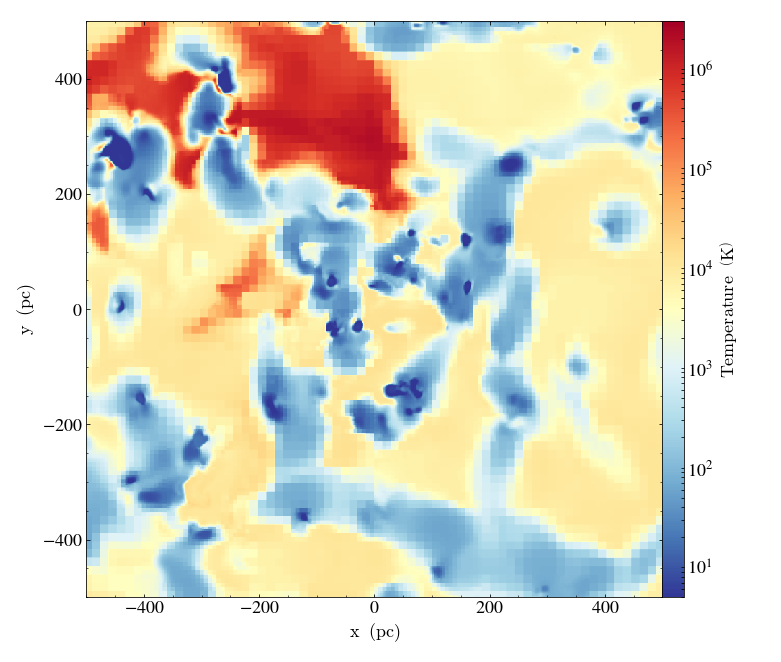
\includegraphics[width=0.32\linewidth]{temperature}\\
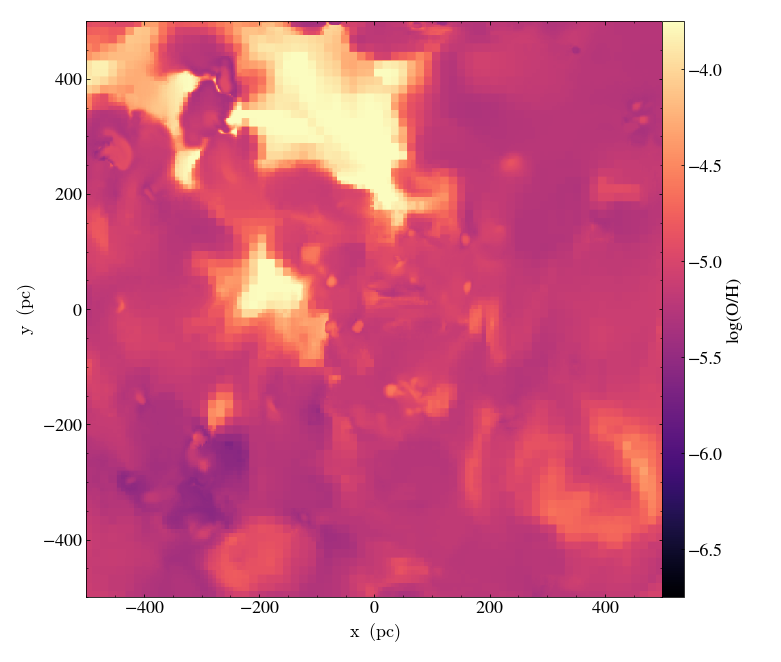
\includegraphics[width=0.32\linewidth]{log_OH} 
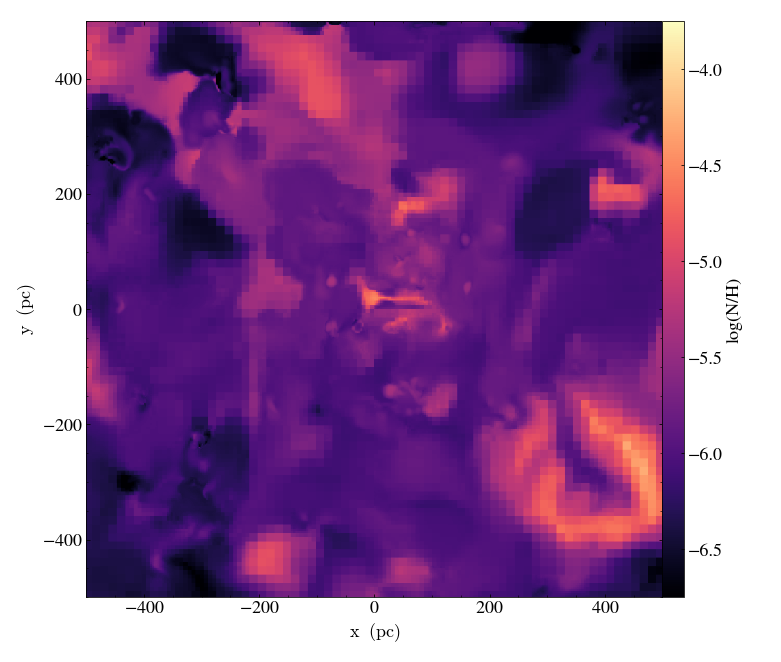
\includegraphics[width=0.32\linewidth]{log_NH}
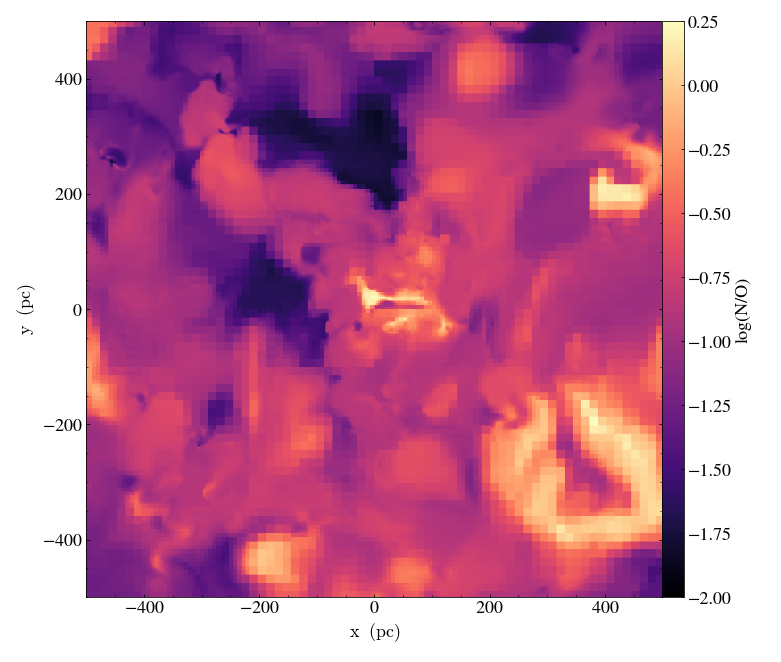
\includegraphics[width=0.32\linewidth]{log_NO}
\caption{Five slices in the mid-plane of our dwarf galaxy at an arbitrary time 
%mm2 [give the time]
  of {\bf XXX}~Myr after the start of star formation,
demonstrating the power of our chemical evolution model. We show the number density and temperature in this region of the galaxy (top row), along with three different elemental abundance ratios, O/H (bottom left), N/H (bottom middle), and N/O (bottom right). We caution against making direct comparisons of these images to observed abundances of dwarf galaxies, as we do not capture a cosmologically realistic chemical evolution in these relatively short ($< 1$~Gyr) simulations. This will be addressed in future work. \textbf{(AE: need to adjust axis label size)}}
\label{fig:metal_slices}
\end{figure*}

Beginning with log(O/H), the gas from the recent SN explosion is abundantly clear, with a higher oxygen abundance by at least 1 dex than its surroundings. The oxygen abundance throughout the rest of the ISM does vary, with 
%mm2 some 
   almost all 
dense regions showing 
%mm2 slightly higher 
   modest enhancements in oxygen abundance compared to their less dense surroundings.
%mm2 , but the variation is not dramatic. 
The ratio log(N/H), however, shows slightly more significant variation throughout the ISM. Comparing the two diagrams, one can pick out regions with differing abundances between the two species. This is clear in the log(N/O) slice, which emphasizes regions with strongly varying abundance in either species. The gas from the SN explosion, for example, has a low log(N/O) due to the significant amount of oxygen released in the SN. Oxygen is generally more abundant than nitrogen throughout the ISM, particularly in the warm, diffuse gas. However, the dense, cold gas typically has a greater log(N/O) than its surroundings, indicating that nitrogen may more easily pollute cold gas than oxygen. These differences are also evident with a few regions of warmer gas (small sliver at center of figure, horseshoe shaped feature in lower right, and the blob in the upper right) where log(N/O) > 0, indicating an overabundance of nitrogen as compared to oxygen. 

%mm2 [new para for the explanation]
At our adopted metallicity, nitrogen is predominantly produced in AGB star winds, with very little production in core collapse supernovae and winds from more massive stars. Therefore, nitrogen is injected into the ISM with significantly less energy ($v \sim 10$~km~s$^{-1}$) than elements produced in supernovae, like oxygen, ($v\sim 10^3$~km~s$^{-1}$). This suggests that the energetic differences between the injection sources can drive abundance variations within the ISM of our dwarf galaxy. 
%mm2 It is possible, then, 
   This suggests
that metal mixing within the ISM (and also metal ejection from the ISM) 
%mm2 is a process 
is species dependent. A more detailed analysis is beyond the scope of this work, but we plan to investigate this point, and potential observational consequences for stellar abundances, in future work. 
% reference my other paper if it is ready-ish by the time I submit this one.

%Observations of Local Group dwarf galaxies have shown that they retain very little of the total amount of metals they are expected to have produced, given their star formation histories (see Section~\ref{sec:observation}). In Figure~\ref{fig:species_fractions} we show the fraction of metals retained within the disk or expelled into the halo of our galaxy over time, along with a breakdown of the locations of each metal species by the end of the simulation. As shown in the top panel, a majority of each metal tracer species is found outside the disk of the galaxy, in the galaxy halo. In total, \textbf{85\%} of the tracer metal species produced lie outside of the disk of our galaxy. Interestingly, the exact fraction is not uniform across metal species. 

%\textbf{Use Ba here as example element, not N}
%Most notably, N is preferentially retained by the galaxy over the other species. Roughly \textbf{35\%} of N produced remains in the disk, as compared to \textbf{15\%} of O or Fe, for example. This difference is entirely feedback driven. At this metallicity, N is produced only in the stellar winds of stars between 8 and 10 M$_{\odot}$, with little to no production in supernovae. The rest of the species either have very little stellar wind production, are produced solely in supernovae, or have similar production levels between both supernovae and stellar winds (like O, for example). The typically lower injection energies of N into the galaxy compared to the SNe produced elements means N is preferentially retained within the ISM, and not as effectively ejected through outflows. In truth, the stars that produce N do eventually explode as supernovae, sweeping up some fraction of the wind produced N into outflows. However, clearly some of this N mixes more effectively within the ISM than the other metal species. How abundance variations like this evolve over longer timescales and with varying feedback physics is the subject of ongoing work.
% AE: possibly cite letter here if we have it done

%\begin{figure*}
%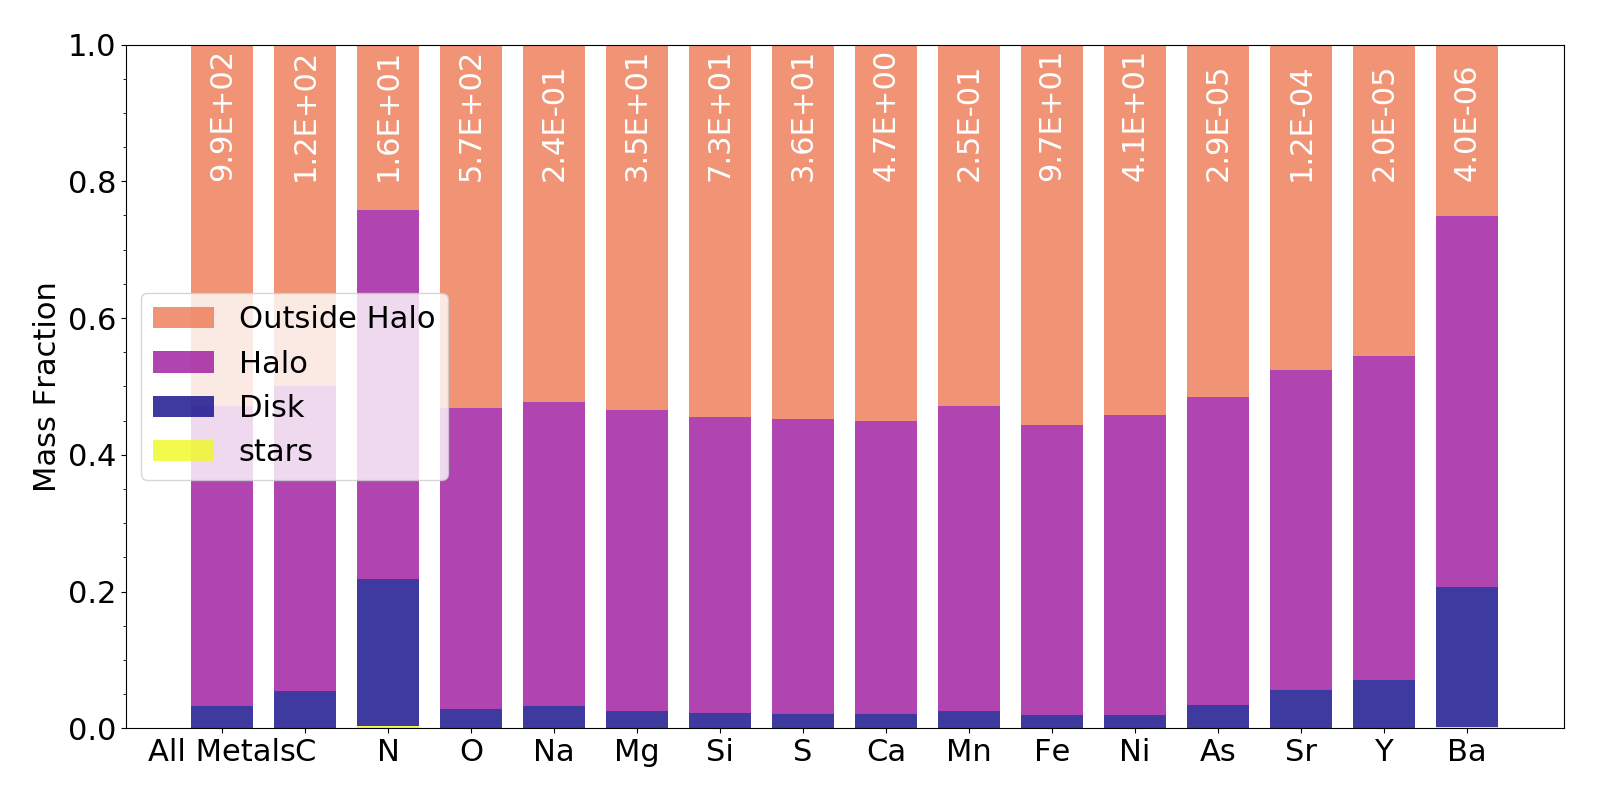
\includegraphics[width=0.9\linewidth]{species_bar.png}\\
%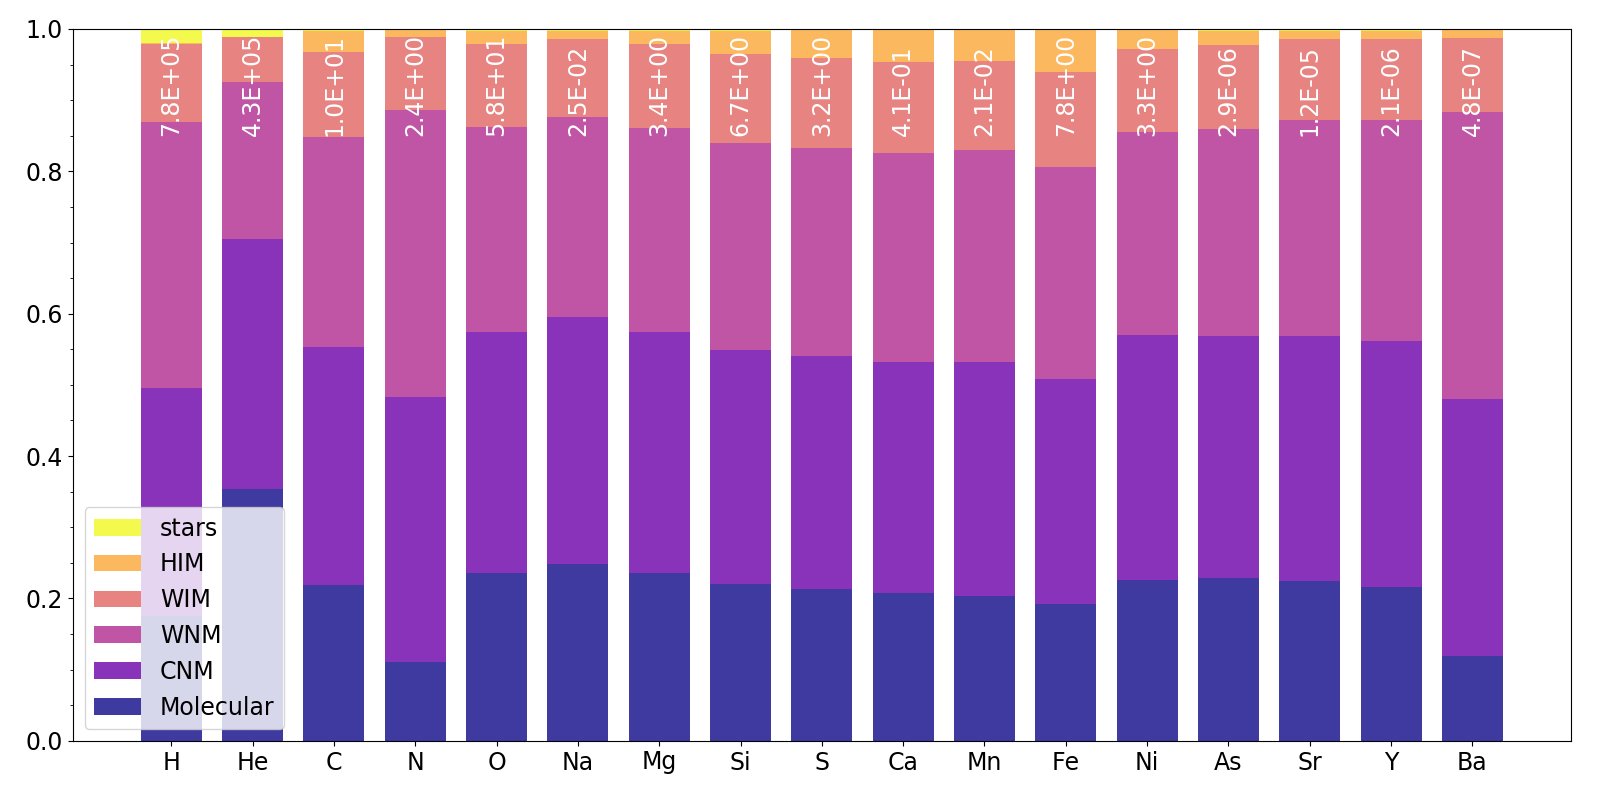
\includegraphics[width=0.9\linewidth]{species_bar_disk.png}
%\caption{The fraction of each species in the full simulation box contained in the halo, gas in the galaxy disk, and stars (top), and the fraction of species within the disk alone in each phase of the ISM (bottom).}
%\label{fig:species_fractions}
%\end{figure*}

%The bottom panel illustrates where these metals are partitioned within the ISM of the galaxy at the end of the simulation time. The CNM contains roughly 50-60\% of each species, with the CNM and WNM together accounting for most of the metals in the galaxy. The WIM contains only $\sim$ 10\% of each species, with the HIM containing very little. This may be counterintuitive given that most metals are initially injected into the galaxy in either the WIM or HIM phases. However, the disk metals represent only a small fraction of the total metals produced. Much of the metals are effectively removed from the disk into the halo (see Section~\ref{sec:outflows}). It is apparent that the remaining metals quickly mix or cool into denser gas phases.

%\subsection{Stellar Abundances}
%\label{sec:stellar properties}

% By initializing the metallicity of our galaxy to a non-zero value (XXX), yet setting each of the metal tracer species to initial mass fractions of 10$^{-20}$ (effectively zero abundance), the species abundances in our galaxy are somewhat contrived. However, this was done to be able to unambiguously follow how self-consistently produced chemical enrichment evolves over time. In effect, what each individual metal field traces is a ``delta'' abundance, or change in metal mass fraction relative to an arbitrary initial condition.

%\textbf{This section needs work. As per discussion with Keith and Kathryn, displaying abundance evolution like this is confusing and misleading. Switch to discussion of mass / abundance fraction evolution of individual specie(s).}
%We plot the $[\alpha / {\rm Fe}]-[\rm{Fe}/\rm{H}]$ ratio for all star particles in our simulation that are ``alive'' in Figure~\ref{fig:stellar_abundance}. This represents stars that have not gone supernovae or have otherwise formed a compact object. Here, $\alpha = (\rm{O} + \rm{Mg} + \rm{Si})/3.0$, and the notation [X/Y] denotes the ratio of the abundance of species X over Y, relative to the solar value, or log([X/Y]) = log(X/Y) - log(X$_{\odot}$/Y$_{\odot}$). All stars are colored by their age.

%\begin{figure}
%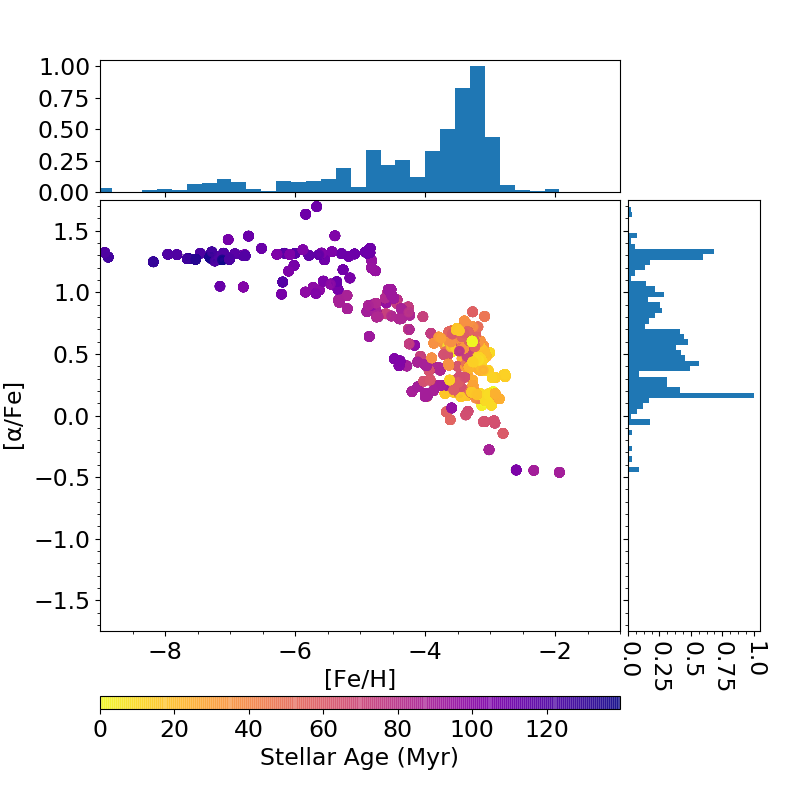
\includegraphics[width=0.95\linewidth]{alpha_over_fe_hist}
%\caption{The $[\alpha / {\rm Fe}]-[\rm{Fe}/\rm{H}]$
%diagram for all stars in our simulation, colored by their age. Here, we define $\alpha = (\rm{O} + \rm{Mg} + \rm{Si})/3.0$. Each histogram shows counts, normalized to the peak in each distribution.}
%\label{fig:stellar_abundance}
%\end{figure}

%As expected, there is a noticeable trend of stellar age with [Fe/H]; especially in our case as the overall iron abundance is gradually increasing, yet we do not have any accretion of primordial material. Interestingly, the few stars with the highest [Fe/H], between -3 and -2, are not the most recently formed; the most recent star formation is clustered around [Fe/H] between -3 and -4.

%We note the ``knee'' like feature at very low [Fe/H] is not the characteristic knee seen in $[\alpha / {\rm Fe}]-[\rm{Fe}/\rm{H}]$ space, corresponding to the period when iron enrichment from SN Type Ia begins to make a significant contribution to the galactic chemical evolution. This generally occurs after roughly 1 Gyr of stellar evolution, far longer than the \textbf{170} Myr simulated here. % The origin of this feature and the longer term chemical evolution of this galaxy will be investigated in a future work.

\section{Discussion}
\label{sec:discussion}

\subsection{Comparison to Observed Low Mass Dwarf Galaxies}
\label{sec:observation}

\subsubsection{Gas and Star Formation}
\label{sec:gas_sf}

The observational sample of isolated, gaseous, low mass dwarf galaxies is limited compared to more massive galaxies, but has improved substantially with recent blind and targeted \ion{H}{1} surveys \citep[e.g.][]{Giovanelli2005, Geha2006, Geha2012, Walter2008, Cannon2011, Haynes2011, Hunter2012, Bradford2015, James2015, Tollerud2015, Sand2015, Wang2017}. However, the sample of isolated, gaseous dwarf galaxies with $M_{*} < 10^{7}$~M$_{\odot}$ remains small. In Figure ~\ref{fig:KS} we show where our galaxy lies relative to the observed Kennicutt-Schmidt (KS) relation and extended Schmidt law (ESL)  for low mass galaxies. In both diagrams, our simulations are given by the colored points, sampled every 1 Myr throughout the entire simulation. Although simple to measure in simulations, these quantities are challenging to directly compare to observations. 

%mm [new para]
We have attempted to make a reasonable analog to how $\Sigma_{\rm sfr}$ and $\Sigma_{\rm gas}$ are measured observationally for low mass dwarfs using the procedure described in \citet{Roychowdhury2014}. We define $\Sigma_{\rm sfr} = \dot{M}_{*,10} / A_{*,10}$, where $\dot{M}_{*,10}$ is the SFR measured over the preceding 10~Myr, and $A_{*,10}$ is the
%mm2 disk defined out to the farthest
   area of the disk within the radius of the outermost 
star formed within the previous 10 Myr. Likewise, $\Sigma_{\rm gas} = M_{\rm gas,10} / A_{*,10}$, where M$_{\rm gas,10}$ is the total gas mass within this defined disk. However, the total gas content cannot be determined observationally. To match this limitation, we follow \cite{Roychowdhury2014} and take $\Sigma_{\rm gas, obs} = 1.34 \times \Sigma_{\rm HI}$, where the factor 1.34 attempts to account for He. There is generally no correction applied to account for any H$_{2}$ or \ion{H}{2} content. The molecular component is discussed further in Section~\ref{sec:molecular gas content}.

\begin{figure*}
\centering
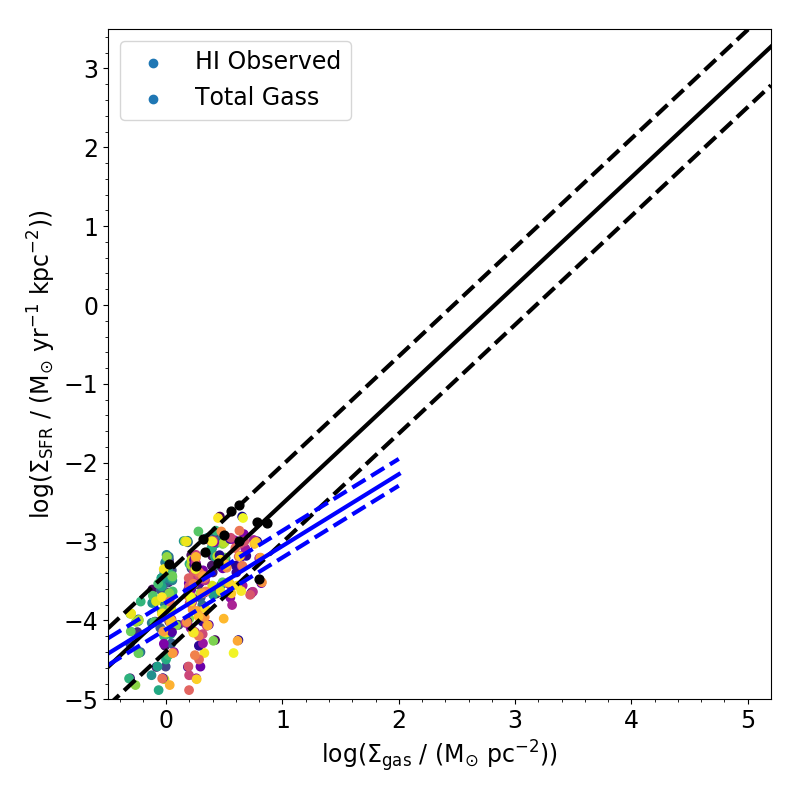
\includegraphics[width=0.475\linewidth]{all_gas_schmidt_law_evolution}
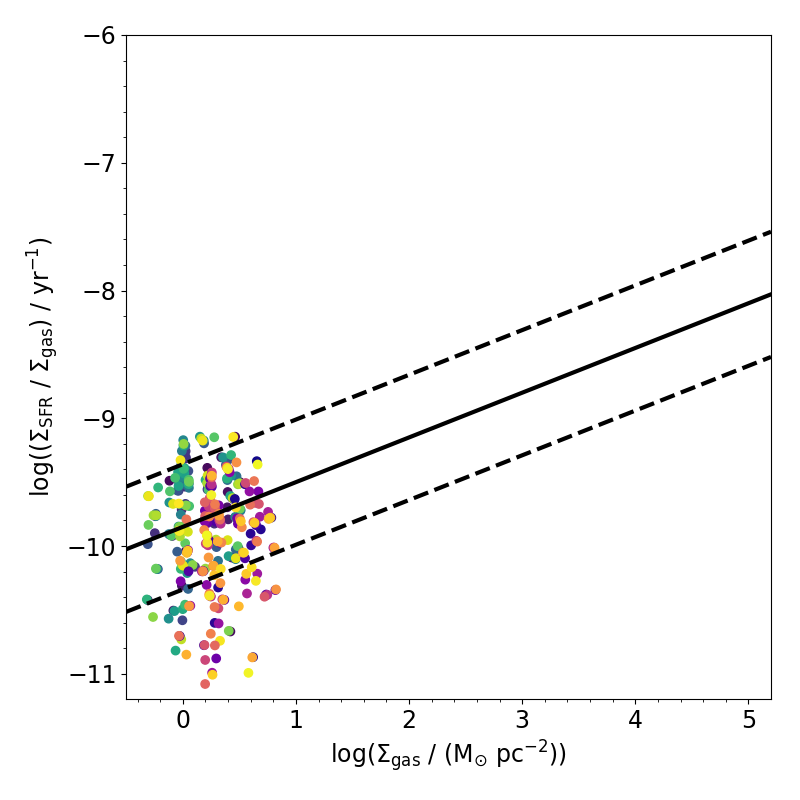
\includegraphics[width=0.475\linewidth]{all_gass_efficiency_evolution}
\caption{The KS law (left) and ESL (right) relationships for our galaxy as measured every megayear, plotted as points colored by time, with dark / purple early and light / green late. 
%mm2 We take $\Sigma_{\rm gas, obs} = 1.34 \times \Sigma_{\rm HI}$ in our simulations to make a fair comparison to the observational sample (see text for more details)
    See text for details of the calculation.
Recent observations from the SHIELD sample \citep{Teich2016} are plotted as 
%mm2 points
    black points with error bars.
On the left, we also give the best fit line to galaxies from the FIGGS sample from \cite{Roychowdhury2014}, and on the right we also show the best fit line and 1 $\sigma$ errors from \cite{Shi2011}.
%mm2  This  is simply to indicate there 
   There
is no clear correlation with time in this diagram.}
\label{fig:KS}
\end{figure*}

%mm2 In both panels, we also 
   We
include recent observational constraints on these relationships
%mm2
    in Figure ~\ref{fig:KS}. 
%mm2 For the KS relationship we 
   These 
include the best-fit line from \citet{Roychowdhury2014}, 
%mm2 (black, dashed). In both we give recent measurements from
the SHIELD galaxy sample \citep{Teich2016}, 
%mm2 (black, points). Recently, \cite{Roychowdhury2017} demonstrated that the best fit line in the ESL from \cite{Shi2011} extends to the low mass FIGGS sample of galaxies; we give this best fit line and 1$\sigma$ errors in the right hand panel (black lines). 
  and the best-fit line with 1$\sigma$ errors from \citet{Shi2011}, which 
  \citet{Roychowdhury2017} demonstrated extends to the low mass FIGGS sample of galaxies.
Our galaxy fluctuates significantly about both relationships with no clear trends in time. However, in both cases, it is consistent with the available observational sample. At times our galaxy exhibits gas surface densities below the observational constraints. The trend is still consistent with higher densities at this point, but with a larger scatter towards lower star formation rate densities and efficiencies.

%mm2 Fig.~\ref{fig:KS} represents a remarkable result. 
In constructing our galaxy model, we employed \textit{no} tuning of the underlying physics, adopting only canonical values for any available free parameters. It is thus non-trivial that our galaxy should oscillate about the median relationships in Fig.~\ref{fig:KS}, and signifies a proper accounting of the relevant physics governing gas and star forming properties in our galaxy. This result is consistent with 
%mm2 recent 
galactic evolution simulations run at high resolution with a detailed accounting of stellar feedback physics (\textit{relevant citations}
%mm2
   starting with A. Kravtsov 2003, ApJ L.)
%mm 
%ae: but does this bit then contradict my statement that this is remarkable? if its 'just gravity' at play?  
%mm2: that's the question, isn't it?  maybe keep the description of the result, but remove the claim of remarkability, as I have edited to do?
   but also with the demonstration by \citet{Li2006} that the KS law can be reproduced 
   by gravitation acting on an isothermal disk, which was argued to demonstrate that 
   this represents the basic physics at work.

\subsubsection{Molecular Gas Content}
\label{sec:molecular gas content}

The molecular gas content of low mass dwarf galaxies is generally assumed
to be small, but is not well constrained by either theory or observations. Assuming the relationship in \citet{Leroy2013} and \citet{Momose2013}, \citet{Roychowdhury2014} finds typical molecular gas fractions anywhere from $f_{\rm H_2} = 0.05$ to $f_{\rm H_2} = 0.5$; a significant range in values. As discussed in Section~\ref{sec:properties}, our galaxy has $f_{H_2}$ of 0.17--0.20, within this range, but significantly exceeding the few percent often found in models. Ignoring the H$_2$ component of our galaxies would lead to an average shift of 0.24 dex to the right in the KS relationship, and 0.24 dex right and down in the ESL. This does not result in a significant disagreement with the observed relationships, but would constitute a quantitative change to the observed fits if our $f_{\rm H_2}$ is robust for observed low mass, low metallicity dwarf galaxies. 

Interestingly, in this low-dust regime, our H$_2$ formation is dominated by the gas-phase reaction H$^-$~+~H~$\rightarrow$~H$_2$~+~e$^{-}$. In our model, H$^{-}$ is produced solely through the reaction H~+~e$^{-} \rightarrow$ H$^{-}$~+~$\gamma$. Prior to the establishment of a local stellar radiation field, e$^{-}$ production is dominated by the ionization of H and He from the ultraviolet background. This has the seemingly counterintuitive effect that turning off the ultraviolet background actually decreases the formation rate of H$_2$, as confirmed in test simulations. In a test simulation ignoring H$^{-}$, we find H$_{2}$ mass fractions on order of  $\sim 5\%$ by first star formation, a factor of 3 reduction from our fiducial model.

This explains our 
%mm2 contention 
    disagreement
with the simulations in \citet{Hu2016} and \citet{Hu2017}, which find low molecular fractions ($f_{\rm H_2} \sim 10^{-4}$) even in their simulations without any feedback ($f_{\rm H_2} \sim 2 \times 10^{-3}$). Although these works do contain a non-equilibrium chemical model, they do not include either H$^{-}$ or a background radiation field. Our model suggests that H$^{-}$ and the ultraviolet background (in the absence of a local radiation field) are critical components in H$_2$ formation in small dwarf galaxies. It is not surprising that the gas phase reactions dominate over grain catalysis in this low metallicity regime \citep{Glover2003}, but the total amount of H$_2$ formed is perhaps surprising. However, the rate coefficients associated with gas-phase H$_2$ formation are uncertain by an order of magnitude \citep{Glover2006,Glover2007}.
%In addition, \cite{Glover2006} demonstrated that the total amount of H$_2$ formed can be quite sensitive to the initial conditions.
%mm2 Finally, our model lacks additional chemistry which 
    Our model does lack additional chemistry that
may be important to the formation and destruction of H$_2$, including HD chemistry, C and O chemistry, a detailed dust model, and cosmic rays. It is unclear how the combination of all of these effects will behave, especially considering that even at this resolution, we are unable to resolve the high density turbulent density perturbations in which H$_2$ forms most efficiently \citep{Glover2007}. This uncertainty certainly warrants further study of molecular gas in low metallicity dwarf galaxies.
%ae rewrote above and took out this citation, need to see if need to put back in:
%            there is some possible observational evidence for higher than expected ($\sim 15$ \%)   %            molecular fractions \citep{Schruba2017}, though this still remains highly uncertain.

\subsubsection{Metal Retention}
\label{sec:obs_metals}

The simulations presented here have not yet been run for the gigayear timescales required to make direct comparisons to the observed stellar and gas phase metallicities of comparable dwarf galaxies at $z = 0$. However, we can compare to a key observable, the retention fraction of metals within stars and the galaxy's ISM compared to what would be expected from
%mm2
  closed box
stellar evolution models based on the galaxy's star formation history. This can be done readily with Milky Way dSph's. Their stars seem to retain very little of the expected metal production: on order of a few percent or less depending on the galaxy and the species \citep{Kirby2011-metals}. However, environmental effects, namely ram pressure and tidal stripping, complicate the understanding of how these metals were removed from the galaxy. 

Leo P, the dwarf galaxy we approximate in our initial conditions, is extremely valuable as a %mm2 gaseous, 
   gas-containing,
star forming, low-mass dwarf galaxy, with an observable \ion{H}{2} region, necessary for determining gas phase abundances, that is close enough to the Milky Way to conduct this experiment. Leo P retains $\sim$ 5\% $\pm$ 2\% of its metals, $\sim$ 1\% in stars and the rest in ISM gas \citep{McQuinn2015}. As discussed in Section~\ref{sec:chemical evolution}, roughly 90\% of the tracked metals produced during our simulation no longer reside within the galaxy's disk. At the end of our simulation, we 
%mm2
   thus
agree with the observations; however, this is an evolving quantity that also depends on how much (if any) subsequent re-accretion of these metals occurs. Although more than half of these metals are expected to eventually re-accrete \citep{Angles-Alcazar2017}, it is still possible that
most of the metals that have been produced at these early times will remain outside the galaxy disk. We will examine the long term, and species-by-species, evolution of the metal retention fraction in future work.

It is interesting to consider whether ejected metals in our model reside in the CGM or have been ejected into the intergalactic medium. While this cannot be observationally determined for dwarf galaxies at this mass, cosmological simulations of a $M_{\rm vir} = 10^{10}$ M$_{\odot}$ galaxy show that, by redshift zero $\sim$ 60\% of ejected gas is recycled, while 40\% is ejected from the galaxy's halo \citep{Angles-Alcazar2017}. In our case, no metals have been ejected beyond the virial radius; this is not surprising however, given that metals ejected beyond the halo would need to travel with an average velocity of 150 km s$^{-1}$ for the entirety of our simulation time.  We find 13.7\% of all metals lie within 1 kpc of the center of our galaxy, 26.5\% within 0.25 $R_{\rm vir}$ (or 6.85 kpc), and 38.6\% outside $R_{\rm vir}$. 

%mm2 [new para]
The re-accretion or final ejection of this gas is directly relevant to the chemical evolution of low mass dwarf galaxies. Recycling of metal enriched gas could be a significant driver of long-term chemical evolution in low mass galaxies, particularly if a majority of metals ejected from the disk (itself nearly all the metals produced by the galaxy) return. Our model seems to suggest that many of the metals ejected into the halo will not be recycled back into the galaxy, but this is difficult to determine with only 500~Myr of evolution. In addition, the accretion of pristine gas from the intergalactic medium could significantly affect the gas flows around the galaxy, possibly promoting the retention of ejected metals. This effect is not included in our isolated galaxy simulations, and its role is beyond the scope of this work.

\subsection{Missing Physics}
Although we include many detailed physical models in our simulations, there remain additional physical processes that may be relevant, which we now discuss.

\subsubsection{Full Stellar Wind Model}
\label{sec:stellar winds discussion}
Our stellar wind model significantly reduces the injected wind velocity from $\sim$1000 km s$^{-1}$ to 1 km s$^{-1}$. Although our model is capable of generating realistic stellar winds with temperature profiles and radial evolution comparable to those expected from analytic calculations \citep{Weaver1977}, the hot, fast winds place a near constant and severe constraint on the Courant time step that renders $\gtrsim$100~Myr simulations impractical. When considered in isolation, stellar winds are an important source of pre-SN feedback and do dramatically influence the dynamical evolution on molecular cloud and galaxy scales \citep{Dale2008,Peters2017,Gatto2017}. However, when considered together with ionizing radiation, stellar winds contain less total energy \citep{Agertz2013} and do not seem to have a significant dynamical influence in either idealized simulations \citep{Geen2015} or 
%mm GMCs
   individual giant molecular clouds
\citep{Dale2014}. They are even less relevant in the low-metallicity regime studied here, as stellar winds become weaker with decreasing metallicity \citep{Puls2000, Vink2005}. Although they likely have minimal dynamical importance
%mm 
   at resolutions where peak densities are not anyway high enough to trap ionization 
   fronts, 
a full model of stellar winds may affect detailed ISM properties and metal mixing, warranting a closer examination in a future work.
%mm2: should we recover the reference to Shull \& Saken?
%old comment: (need to ref or back up this claim: see Dale et al. 2014 for individual clouds, while the right panel of Fig 2 in Shull \& Saken 1995 shows that the integrated wind energy from a cluster is about 10\% that of the supernovae -M). 

\subsubsection{Cosmic Rays} 
%mm2 and Magnetic Fields}  One could make the case that we should have a separate discussion of magnetic fields.  However, this section is only about CRs.

Recent work has explored the importance of cosmic ray feedback in regulating the ISM and wind properties in galactic disks \citep{Hanasz2013,GirichidisCR,Simpson2016,Farber2017}, isolated galaxies \citep{SalemBryanCorlies,Salem2015,Pakmor2016,Ruszkowski2017}, and galaxies in cosmological context \citep{SalemBryanHummels}. These relativistic charged particles act as a source of non-thermal pressure support in the galaxy's ISM, capable of driving outflows at different velocities and containing different thermal phases than those driven through thermal feedback alone \citep{SalemBryanCorlies}. Modeling cosmic rays is challenging, however, as they encompass a wide range of energies,
%mm2 (give range), with 
   and there are
significant uncertainties in how they propagate through the ISM \citep[e.g.][]{Wiener2017}. Their propagation is often modeled as a diffusive process, but in truth this diffusion should vary depending on cosmic ray energy. In addition, cosmic rays couple effectively to the magnetic fields of galaxies, diffusing preferentially along structured magnetic field lines within the ISM. Modeling cosmic ray feedback completely thus requires both an accurate cosmic ray model and magnetohydrodynamics in order to capture the interplay of these two physical phenomena. Finally, including MHD presents additional difficulties in untangling the effects of each individual feedback mechanism on galaxy chemodynamics.

We do note that an isotropic, two-fluid model for cosmic ray feedback exists in  \textsc{Enzo} \citep{SalemBryan2014,Salem2015} and has been well tested. Mechanically, including cosmic ray feedback in our model is trivial. However, the cosmic ray population, their diffusion coefficient, and the magnetic field structure of the lowest mass dwarf galaxies each have significant enough uncertainties to warrant reserving their full inclusion into our model to a later work.

%\subsection{Detailed Dust Model}
%\textbf{Should we discuss this? If so I definitely need more info and references - AE}.
%The dust content of our galaxy is modeled only approximately, scaling with the cell-to-cell variations in gas metallicity. Explicitly following the dust content in our galaxy, even crudely, could introduce significant variations in local cooling and heating rates. Accounting for metals trapped in a dust phase would produce additional variations in the cooling rates and potentially changes to the galactic chemodynamical evolution. 

\subsection{Detailed Stellar Evolution and Binary Stars}
\label{sec:binary stars}
% Although we track individual stars and assign properties to each based on stellar evolution models, these properties are fixed. A more detailed model could follow each star on an interpolated stellar evolution track, which would account for variations in radiation and stellar wind properties in each star over time. 

Roughly half of massive stars live in binary pairs 
%mm2 doi:10.1051/0004-6361/201219621
   \citep{Sana2012}. 
Their interactions, primarily through mass transfer, can significantly alter their radiation properties and lifetimes. This can change both how much and how long these stars emit ionizing radiation, an important source of stellar feedback, and where and when these stars explode as supernovae. This effect is rarely accounted for in galaxy evolution models, which are commonly based on calculations of single star evolution (e.g. STARBURST99), but could be significant. For example, \citet{Zapartas2017} finds that binarity extends the timescales over which core collapse supernovae occur from a given star formation event, from a maximum time of $\sim$ 50~Myr to $\sim$~200~Myr. Although they find only $\sim 15\%$ of core collapse supernovae explode after 50~Myr, this could still be an important effect. Properly accounting for the delay times due to variations in individual star lifetimes has already been shown to change the significance of feedback and influence galaxy metallicity properties \citep{Kimm2015}. Extending the lifetimes of these stars could increase the role of radiation feedback, however this may be less important as these additional photons are more likely to escape the galaxy \citep[e.g.][]{Ma2016-binary}. 
% does this affect yields??
% runaway stars

Since we model stars on a star-by-star basis, both of these effects could be reasonably accounted for by stochastically assigning binary star properties to some subset of our individual stars. This is beyond the scope of this project, but will be investigated in future work.

\section{Conclusion}
\label{sec:conclusion}
We have developed a new method for simulating galaxy evolution with detailed feedback and chemical enrichment. For the first time on galaxy scales, we simultaneously model multi-channel stellar feedback in detail, accounting for stellar winds, core collapse and Type Ia supernovae, ionizing radiation followed through radiative transfer, photoelectric heating, and Lyman-Werner radiation using individual star particles. This, coupled with the detailed chemistry and heating/cooling physics followed with \textsc{Grackle}, allows us to capture realistic galaxy evolution in detail. In this work, we apply these methods to simulate the evolution of an isolated, low-mass, dwarf galaxy modeled after the $z=0$ properties of the Leo P ultrafaint dwarf galaxy. We present an overview of the properties of this 
%mm2 galaxy
    simulation 
in this work.
% AE: mention companion paper here if publish at same time

For our simulated dwarf galaxy, we find:
\begin{enumerate}
\item Multi-channel feedback is effective in this galaxy in regulating star formation 
%mm2 
   to occur at a rate 
consistent with the KS relationship and extended Schmidt law in observed galaxies. See Figures~\ref{fig:sfr_mass_evolution} and \ref{fig:KS}.

\item This feedback drives large outflows 
%mm2 ($\eta \sim 50$ at 0.25~R$_{\rm vir}$) with
   having mass loading factors of $\eta \sim 50$ at 0.25~R$_{\rm vir}$, and
metal mass loading factors near unity. By mass, nearly all of this outflow is moving with velocities below 100 km~s$^{-1}$, but there is a significant tail towards velocities up to 1000 km s$^{-1}$ (Figure~\ref{fig:outflow_velocity}). 

%mm2 [made this a separate item]
\item 
%mm2 This galaxy result is consistent with the observed metal retention fractions of ultrafaint dwarfs, retaining only $\sim$10\% of metals in the disk. 
    Only $\sim$10\% of metals are retained in the disk of our simulated galaxy, consistent with the observed metal retention fractions of ultrafaint dwarfs.  By the end of the simulation $\sim$50\% of the remaining metals remain within the virial radius and $\sim$40\% 
have been ejected beyond the virial radius. The fraction in the disk remains fairly constant towards the end of the simulation, but the metals in the halo are still evolving. See Figures \ref{fig:mass_outflow}, \ref{fig:outflow_velocity}, and \ref{fig:metal_evolution}.

\item A thin, yet resolved, gas scale height ($\sim 50$~pc) beyond our stellar radius, with larger scale heights ($\sim 100$--200~pc) driven by feedback interior to the stellar radius. This is comparable to the resolution limit of the diffuse \ion{H}{1} in observed, gaseous ultrafaint dwarfs. See Figure~\ref{fig:scale_height}.

\item The ISRF of our galaxy is highly varying in time, by orders of magnitude, though it is relatively uniform in space at any given time. It is unclear how important these fluctuations are as a source of feedback, or if the affect can 
%mm2 simply 
be approximated with a time averaged radial profile. See Figures \ref{fig:ISRF} and \ref{fig:ISRF_2D}.

\item Formation of a significant amount of H$_2$ through gas phase reactions with H$^-$. This dense gas is more resistive to feedback driven outflows than the less dense gas in the galaxy. This leads to high molecular gas fractions, with an H$_2$ mass comparable to that of \ion{H}{1} by the end of the simulation. This result requires further investigation to determine if this behavior is universally true of ultrafaint dwarf galaxies. See Figure~\ref{fig:ISM_evolution}.
\end{enumerate}

Finally, we used O and N as examples to briefly demonstrate that there are discernible differences in how individual metal species are distributed within the ISM of our galaxy. In future work we will investigate in detail how metal enrichment proceeds in low mass dwarf galaxies, including how metals move through the various phases of the ISM into star forming gas, and how individual metals move 
%mm2 through the halos of low mass dwarf galaxies.
  into halos. 
% In addition, we will investigate 
   This will allow us to examine
the role each of our sources of feedback plays in driving dwarf galaxy chemodynamics.

\section*{Acknowledgements:} A.E. is funded by the NSF Graduate Research Fellowship DGE 16-44869. 
We gratefully recognize computational
resources provided by NSF XSEDE through grant number TGMCA99S024, \textbf{need Pleiades alloc}, Columbia University, and the \textbf{(need proper ack. for Simons computing resources)}. Analysis in this work
made significant use of the publicly available \textsc{yt} (http://ytproject.org)
toolkit. \textsc{Enzo}, \textsc{Grackle}, and \textsc{yt} are the products of a collaborative effort of many independent scientists from numerous institutions around
the world. Their commitment to open science has helped make
this work possible
We would also like to thank for their advice and valuable conversations: John Wise, Brian O'Shea, Benoit Cote, Britton Smith, Simon Glover, Kathryn Johnston, Mary Putman, Keith Hawkins, Joshua Wall, and Chia-yu Hu. \textbf{AE: is this too many people? I do think they all deserve acknowledgement. (list is in no particular order).  MM: I'd alphabetize and use first initials following ApJ style, but fine by me to keep everyone on.}

\textit{Software:} \textsc{Enzo} \citep{Enzo2014}, \textsc{yt} \citep{yt}, \textsc{Grackle} \citep{GrackleMethod}, \textsc{Cloudy} \citep{Cloudy2013}
%\bibliographystyle{apj}
%\bibliography{msbib}

\bibliographystyle{yahapj}
\bibliography{msbib}

\appendix
\renewcommand\thefigure{\thesection.\arabic{figure}}    
\setcounter{figure}{0}

\section{Gas Phases of the ISM}
\label{appendix:phases}

To aid in comparison to other works, we define our ISM phases here, as adopted from \citet{Draine2011} Table 1.3 and used consistently throughout this analysis. By construction, these phases are mutually exclusive. In the below, $f_{\rm H_2}$ is the molecular hydrogen fraction by abundance.

\begin{enumerate}
\item Hot Ionized Medium (HIM): $T \geq 10^{5.5}$ K
\item Warm Ionized Medium (WIM): $10^{4}~\rm{K} \leq T < 10^{5.5}~\rm{K} $
\item Warm Neutral Medium (WNM): $10^{2}~\rm{K} \leq T < 10^{4}~ \rm{K}$
\item Cold Neutral Medium (CNM): $T < 10^2$ K, $f_{\rm H_2} \leq 0.5$
\item Molecular: $T < 10^2$, $f_{\rm H_2} > 0.5$
\end{enumerate}

\section{Stellar Radiation Properties}
\label{appendix:radiation}
We detail the radiation properties of our model stars as a function of stellar mass and metallicity, both of which are assigned directly from an IMF and from the local gas properties respectively. The stellar radiation properties are determined from the OSTAR2002 grid \citep{Lanz2003} in the regime that it covers, or integrated from an adjusted black body curve 
%mm off of the OSTAR2002 grid) 
    for other stars,
given the ZAMS stellar radius obtained from the PARSEC \citep{Bressan2012,Tang2014} stellar evolution data set. In Figure~\ref{fig:stellar radiation properties} we plot these properties. We use a constant factor across metallicities for stars not sampled on the OSTAR2002 grid to shift the black body radiation fluxes to be roughly continuous with the ionizing photon rates and luminosities as a function of stellar mass. This requires two factors for each radiation type, one for low mass and one for high mass stars. We use the following multiplicative factors to adjust the black body spectrum for \ion{H}{1} and \ion{He}{1} radiation respectively: [0.1, 3.2] and [0.0001, 4.0]. We do not find this adjustment to be necessary for the FUV and Lyman-Werner radiation bands.

The ionizing radiation photon energies are taken as the average ionizing photon energy for a black body of the star's given T$_{\rm eff}$ obtained from the PARSEC grid. A more accurate approach to compute this energy would convolve the full stellar spectrum and the frequency-dependent absorption cross section. We tested this approach using the frequency-dependent photoionization cross sections from \citet{1996ApJ...465..487V}.\footnote{Source code containing the analytic fits given in \citet{1996ApJ...465..487V} was obtained from \texttt{http://www.pa.uky.edu/~verner/photo.html}} The black body approximation is accurate to within 5\%, yet substantially easier to compute on the fly as integrals over the black body spectrum can be expressed as infinite series that rapidly converge to high precision. Unlike for the ionizing radiation, we assume constant FUV and Lyman-Werner band energies for each star, at 9.8 eV and 12.8 eV respectively.


\begin{figure}
\centering
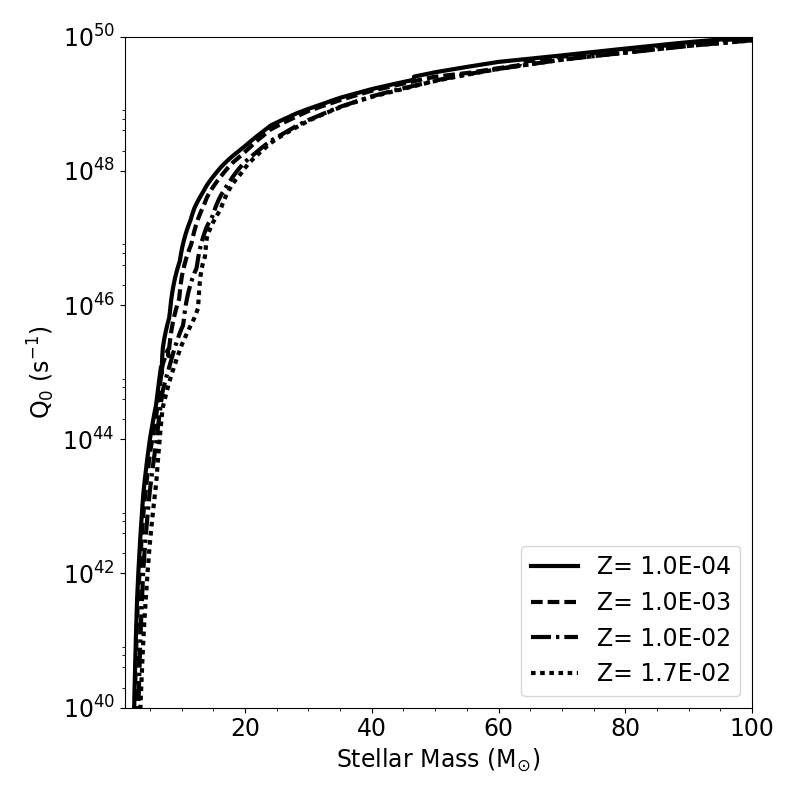
\includegraphics[width=0.4\linewidth]{Q0}
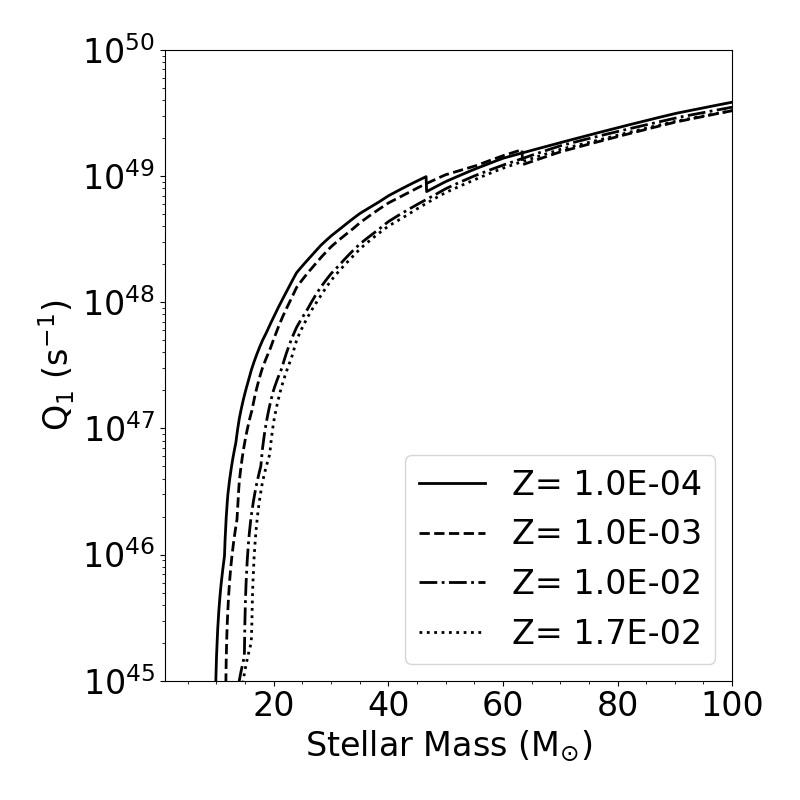
\includegraphics[width=0.4\linewidth]{Q1}
\vspace{0.01cm}
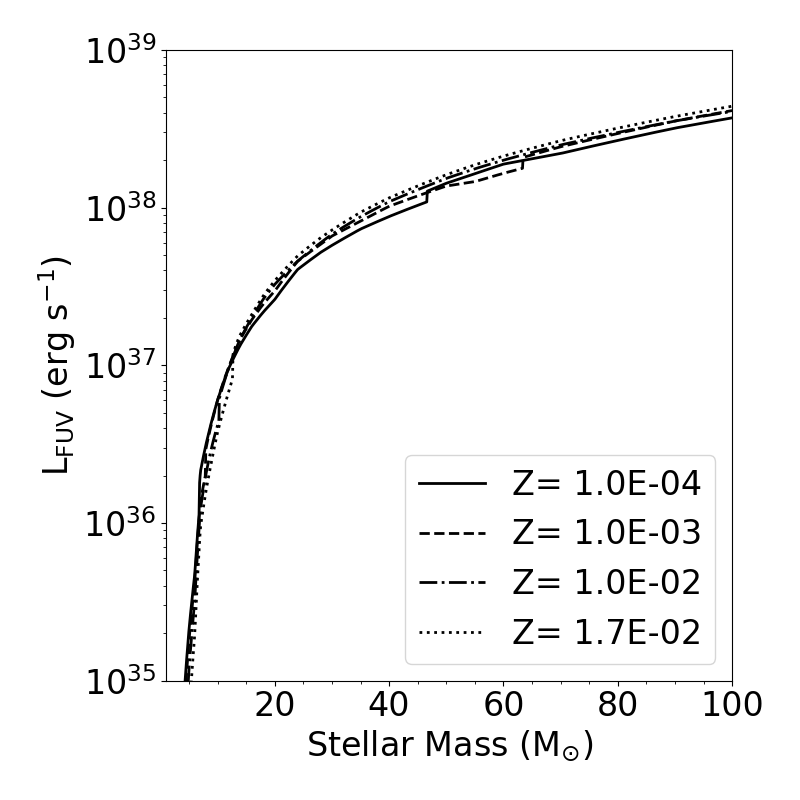
\includegraphics[width=0.4\linewidth]{L_FUV}
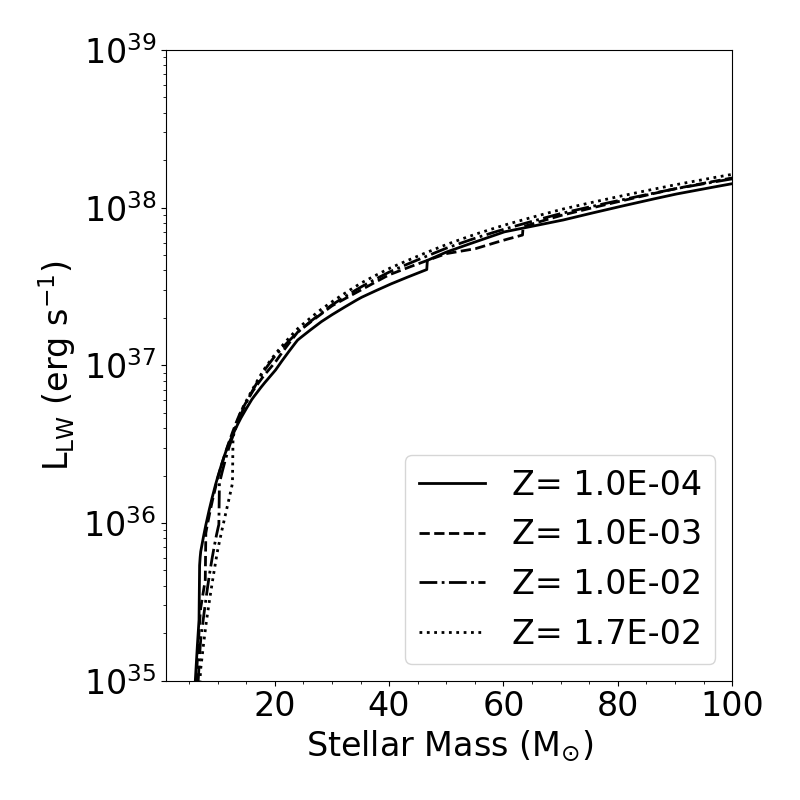
\includegraphics[width=0.4\linewidth]{L_LW}
\vspace{0.01cm}
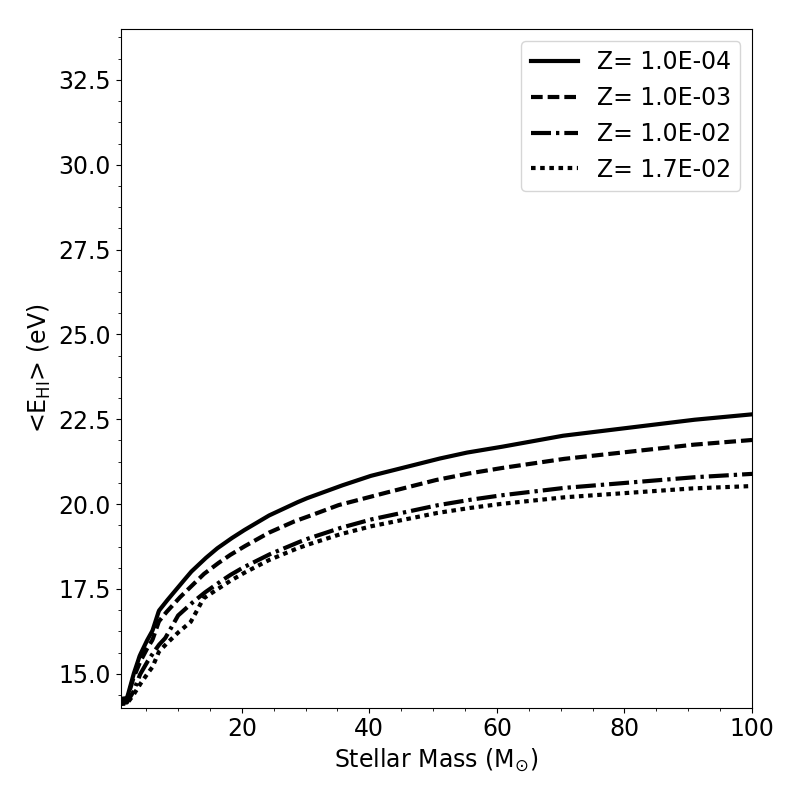
\includegraphics[width=0.4\linewidth]{E0}
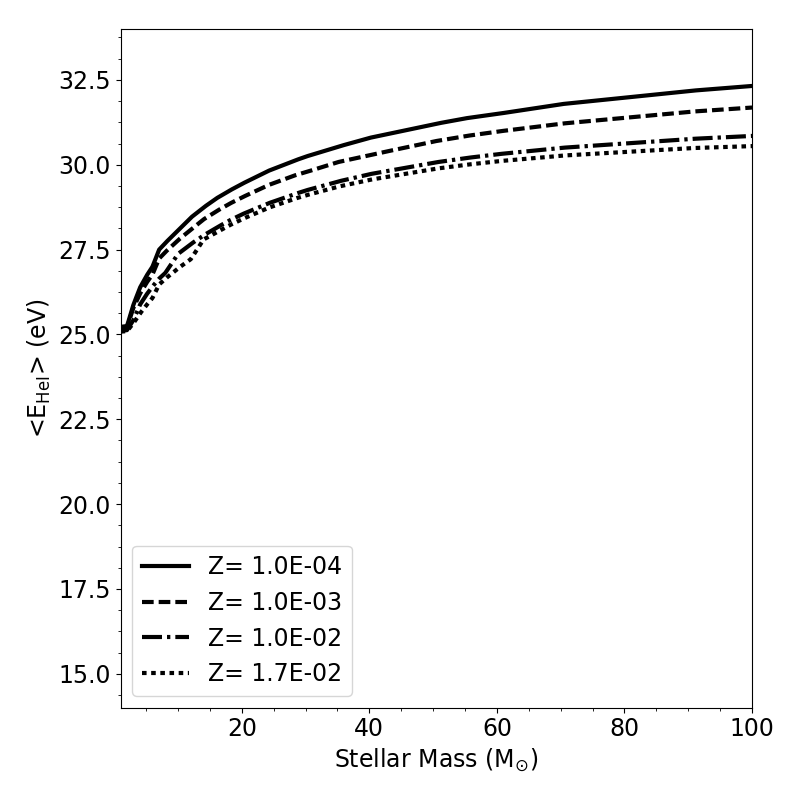
\includegraphics[width=0.4\linewidth]{E1}
\caption{Radiation properties for our model stars, showing the ionizing photon luminosities for \ion{H}{1} (top left) and \ion{He}{1} (top right) for each star, the FUV (middle left) and Lyman-Werner (middle right) luminosities, and finally the average ionizing photon energy for \ion{H}{1} (bottom left) and \ion{He}{1} (bottom right). Note, we only track radiation from stars above 8.0 \msun, which dominate over less massive stars, even when accounting for IMF weighting.}
\label{fig:stellar radiation properties}
\end{figure}

\section{Typical Gas Densities in Supernova Injection Regions}
\label{appendix:supernova}

Modeling supernova feedback with the injection of thermal energy alone can lead to rapid overcooling of the injected energy, and a significant underestimate of the effects of supernova feedback. Often, ad hoc solutions to this problem are used in large simulations with coarse resolution, such as momentarily turning off cooling in feedback affected regions or decoupling affected regions from the hydrodynamics for some time. However, physically consistent solutions have been developed \citep[e.g][]{Simpson2016} that inject a mixture of kinetic and thermal energy with a ratio that depends on resolution and local gas density. 
%mm This overcooling problem improves 
   Overcooling becomes less important 
with higher resolution and lower ISM densities, until eventually pure thermal energy injection is sufficient to resolve each supernova. We take advantage of our high (parsec scale) resolution and employ a simple thermal energy injection model for our supernova feedback. We demonstrate how well this resolves our supernovae in the comparison simulation presented in this work.

The left panel of Figure ~\ref{fig:supernova histogram} gives the distributions of the peak and average ISM number densities in the supernova injection regions for each supernovae in the simulations presented in this work. As shown, a majority explode in regions at substantially lower densities than the star formation threshold of 200~cm$^{-3}$. For most supernovae, $n_{\rm max} \le 1.0$~cm$^{-3}$, which is due to the substantial pre-supernova feedback included in our simulations. The right panel of Figure ~\ref{fig:supernova histogram} gives the fractional distribution of the calculated radius of the pressure-driven snowplow ($R_{\rm PDS}$) phase of the Sedov-Taylor expansion, adopting the definitions from \citet{Simpson2016}
\[
R_{\rm PDS} = 
\begin{cases*}
49.3E^{1/4}_{51}n^{-1/2}_{o} & if  Z $\le$ 0.01 \\
18.5E^{2/7}_{51}n^{-3/7}_{o}Z^{-1/7} & if  Z $\ge$ 0.01 \\
\end{cases*}
\]
where $E_{51}$ is the injection energy in units of 10$^{51}$~erg, $n_{o}$ is the number density of the medium, and $Z$ is the metallicity in units of $Z_{o}$. \citet{Simpson2016} found that $R_{\rm PDS} > 4.5 \Delta x$ is needed to resolve the supernova explosion with thermal energy injection alone, assuming uniform density in the injection region. In practice, the injection region is never uniform. We give $R_{\rm PDS}$ assuming uniform density at both the average and maximum number density in the injection region of each supernova. As shown, a majority of supernovae are resolved (to the right of the 4.5$\Delta x$ line), but that up to 10\% are somewhat under-resolved. In general, these are supernova explosions from the most massive (i.e. most prompt) stars. We do not expect that resolving these supernovae will dramatically alter our results, but note that simulations presented in future work will examine lower mass galaxies at higher resolution than those presented here. In those, the supernovae are more resolved, but we note that using our feedback model at resolutions much less than 2 pc will require adopting a different injection mechanism. 

% We use a spherically symmetric thermal dump method of modelling supernova explosions. This is the simplest method possible, but can often result in rapid overcooling of the heated gas, effectively underestimating the effectiveness of supernova feedback. Solutions to this problem can often be ad hoc (e.g. briefly turning off cooling) in low resolution, large cosmological simulations. However, recent work has shown injecting some fraction of this thermal energy directly as kinetic energy or momentum alleviates this issue without sacrificing physical realism. However, it has been shown that simple thermal energy injection is sufficient for parsec scale (or better) resolutions, provided the supernova do not occur in very high density regions; if resolved, thermal injection converges with kinetic energy / momentum injection methods. Resolving these explosions with thermal energy injection alone depends ultimately on the grid resolution, background density and ISM structure, the background cooling/heating physics used, and the size and shape of the injection region. Here, we perform a resolution test of our thermal injection method over four uniform densities (0.1 \ccunit, 1.0 \ccunit, 10.0 \ccunit, and 100.0 \ccunit) for both a 8.0 \msun and 25.0 \msun star, comparing to both the analytic solution and results using kinetic energy injection from \citet{Simpson2015}. These results are presented in Figure~\ref{fig:supernova tests}. We note these are heavily idealized cases. In general in our simulations, pre-SN feedback from stellar winds and radiation will reduce the typical densities within which our supernova explosions occur. In addition, supernova will generally be clustered, meaning each SN will reducing the typical density for each subsequent SN in that region. In Figure~\ref{fig:supernova histogram} we plot a histogram of the typical peak and average gas densities in the 3 cell injection region of each supernova in the XXXX XXXXX simulation. As shown, some of the supernova explode in high density regions around 100 \ccunit and are likely under-resolved, but a majority will be resolved.

\begin{figure}
\centering
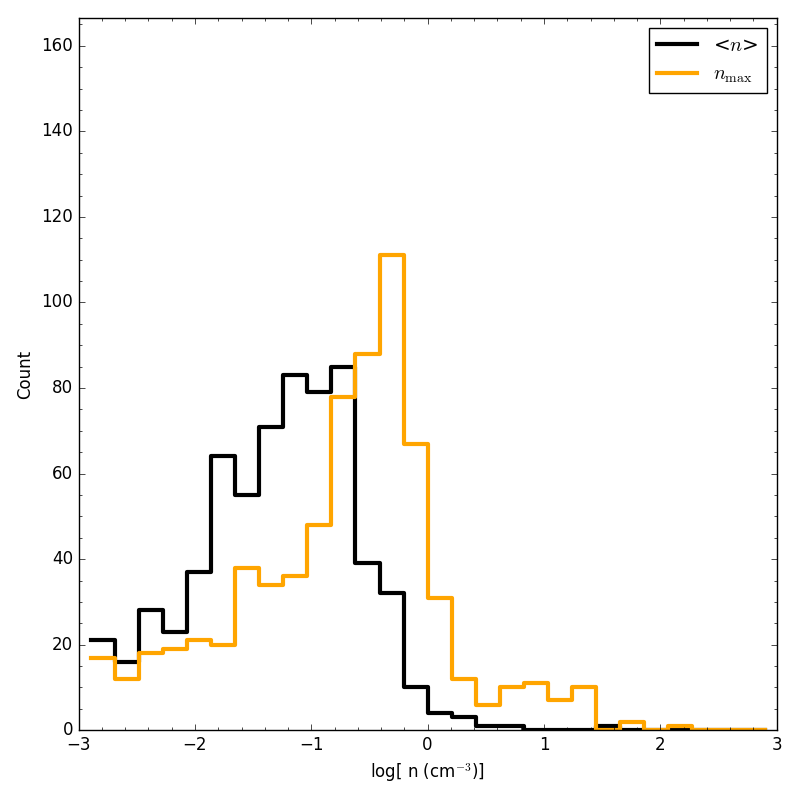
\includegraphics[width=0.4\linewidth]{sn_density_hist}
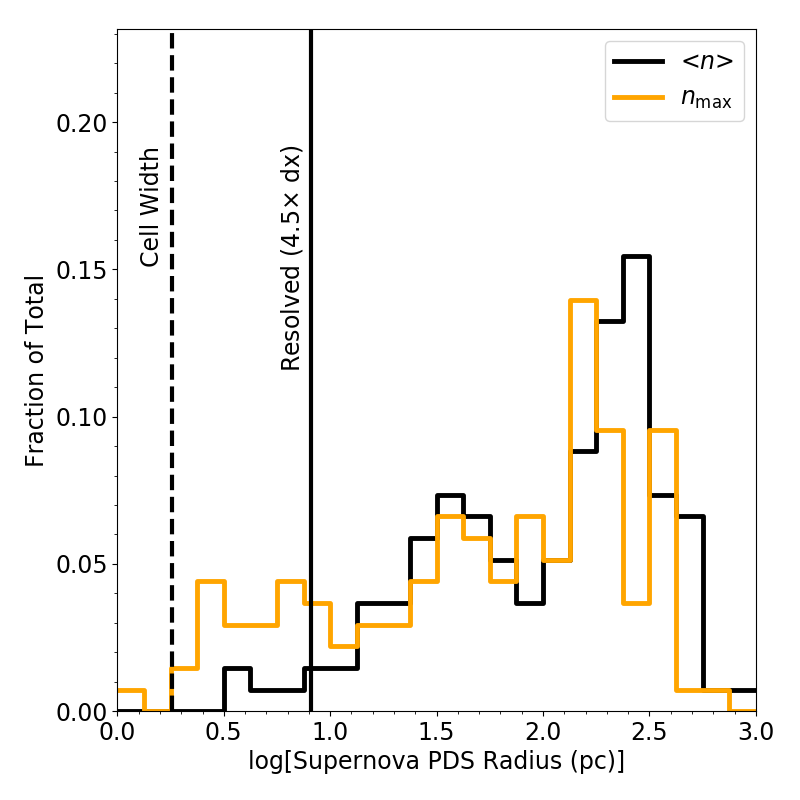
\includegraphics[width=0.4\linewidth]{sn_radius_hist}
\caption{{\em Left:} Distribution of peak (orange) and average (black) gas densities in the injection region of each of the supernovae from the simulation. {\em Right:} Distribution of the radius of the pressure-driven snowplow phase for each supernova assuming a uniform medium at either the peak or average density in the injection region. The vertical lines show one and 4.5 cell widths. This shows that a fraction of these supernovae are certainly under resolved, with R$_{\rm PDS}$ less than a single cell size, but the majority are well resolved.}
\label{fig:supernova histogram}
\end{figure}

%\section{Stellar Wind Model}
%\label{appendix:stellar winds}
%
% This is still probably a good idea to do at some point, but save for if/when
% we have a paper using full stellar winds where this matters - AE (Jul. 19 2017)
%
%Discuss wind properties and evolution in a hand full of isolated star runs (don't need to do a resolution study... kinda) and compare to Weaver et. al. 1977 analytic results. Really we won't resolve the winds at high densities, but that is OK... as long as the wind bubbles are > 3*dx (the injection size) we are generally going to be fine... aka as long as the SN explosion goes off in wind bubble gas and not dense ISM that shouldn't be there..

\section{Cooling and Heating Rates}
\label{appendix:cooling}

%mm moved this paragraph to the start of the section and rewrote accordingly.
To derive the diffuse cooling and heating rates used in the simulations, we make two approximations. First, the primordial cooling and heating rates shown here are those returned by \textsc{Cloudy}, but only the tabulated \textsc{Cloudy} metal-line cooling and heating rates are used. The primordial heating and cooling rates are calculated self-consistently using the non-equilibrium chemistry solver and the self-shielding approximation from radiative transfer simulations given in \citet{Rahmati2013}. However, given that we remove the optically thin assumption when computing the \textsc{Cloudy} tables, the rates shown should be comparable to the locally varying cooling curve in the simulations. Second, this figure ignores the contributions to the heating rate from the variable interstellar radiation field, namely the stellar contribution to photoelectric heating, heating from Lyman-Werner dissociation, and ionization heating. We describe how we obtain the metal line cooling rates below and quantify the change in using these updated tables. 
%Therefore, the heating rates shown are approximate lower limits to the true heating experienced by any given cell in the simulation.

Figure ~\ref{fig:cooling} shows the combined primordial and metal line cooling and heating rates at three characteristic densities for $Z = 0.01 $Z$_{\odot}$, closer to the metallicities of our fiducial set of dwarf galaxy simulations (Emerick et al.\ in prep). The 
%mm solid lines give the absolute value of the net cooling rate, which more clearly 
    Figure 
indicates the regime at low temperatures where heating dominates over cooling. The curve as shown includes 
%mm [it neglects local FUV]
   only
the $z = 0$ \citet{HM2012} metagalactic UV background.

\begin{figure}
\centering
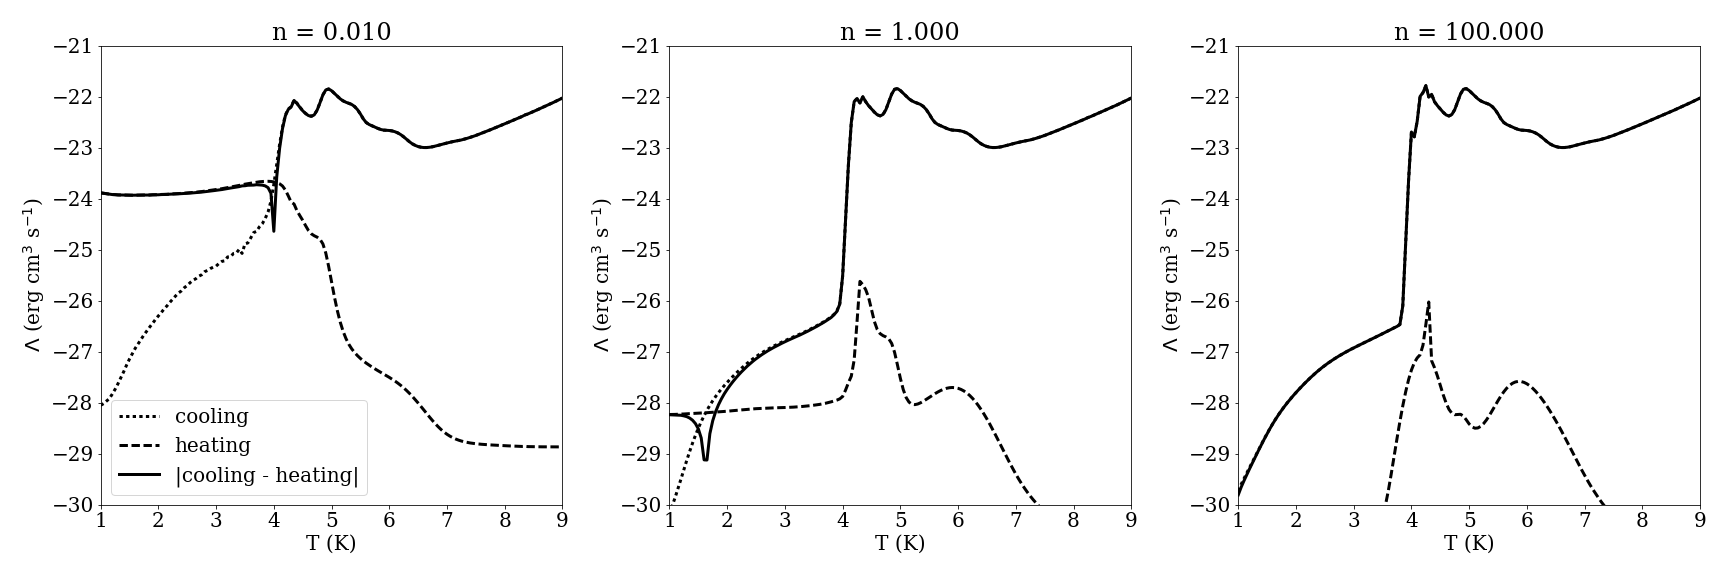
\includegraphics[width=0.95\linewidth]{cooling_curve}
\caption{The total heating (dotted) and cooling (dashed) rates extracted from the core of a Jeans-length sized cloud irradiated by a \citet{HM2012} metagalactic UV background as modeled in \textsc{Cloudy}. The absolute value of the net cooling
%mm
   or heating
rate is shown with solid lines.}
\label{fig:cooling}
\end{figure}

The cooling curves used in this work include a correction to a significant conceptual inconsistency one may encounter when using tabulated metal line cooling rates in combination with self-shielding approximations. \citet{Hu2017} detail this inconsistency: adopting tabulated metal cooling rates computed under the assumption of an optically thin UV background overestimates the electron fraction in regimes where self-shielding is important, about $-0.5 \leq \rm{log(n~[cm^{-3}])} < 2$, leading to an overestimation of the metal cooling rates. We demonstrate this effect in Figure~\ref{fig:cooling comparison}, which gives the absolute value of the net cooling rate
%mm |cooling - heating| 
for our full model at $Z = 0.1$Z$_{\odot}$ as compared to a model using the optically thin metal line cooling rates at a range of densities. The effect is most significant at moderate densities, where the net cooling rate can be an order of magnitude higher. In low temperature regions, this can significantly shift the inferred equilibrium temperature.

The cooling curve shown in Figure~\ref{fig:cooling} avoids this discrepancy using re-computed metal line cooling tables. We have made these tables publicly available in the main distribution of \texttt{Grackle}. For densities where self-shielding is important, we computed \texttt{Cloudy} models of one-dimensional clouds at each temperature and density pair with a physical size corresponding to the Jeans length. In cases where the Jeans length is very large, we limit the size to 100 pc, a reasonable approximation for the maximum size of a self-gravitating cloud. We then adopt the metal line cooling rates obtained from the center of these clouds, whose outside is exposed to the UV background. These models were computed with a modified version of the \texttt{CIAOLoop}\footnote{https://bitbucket.org/brittonsmith/cloudy\_cooling\_tools (our version: https://github.com/aemerick/cloudy\_tools)} code used in \citet{2008MNRAS.385.1443S}. In computing these tables we had to include the cosmic ray ionization that dominates in optically thick clouds. Without this effect, \texttt{Cloudy} becomes unstable in entirely neutral regions. We adopted a cosmic ray ionization rate of 10\% the Milky Way value, though we note that varying this from 1\% to 100\% the Milky Way value did not have an effect on the extracted metal line cooling rates. 

\begin{figure}
\centering
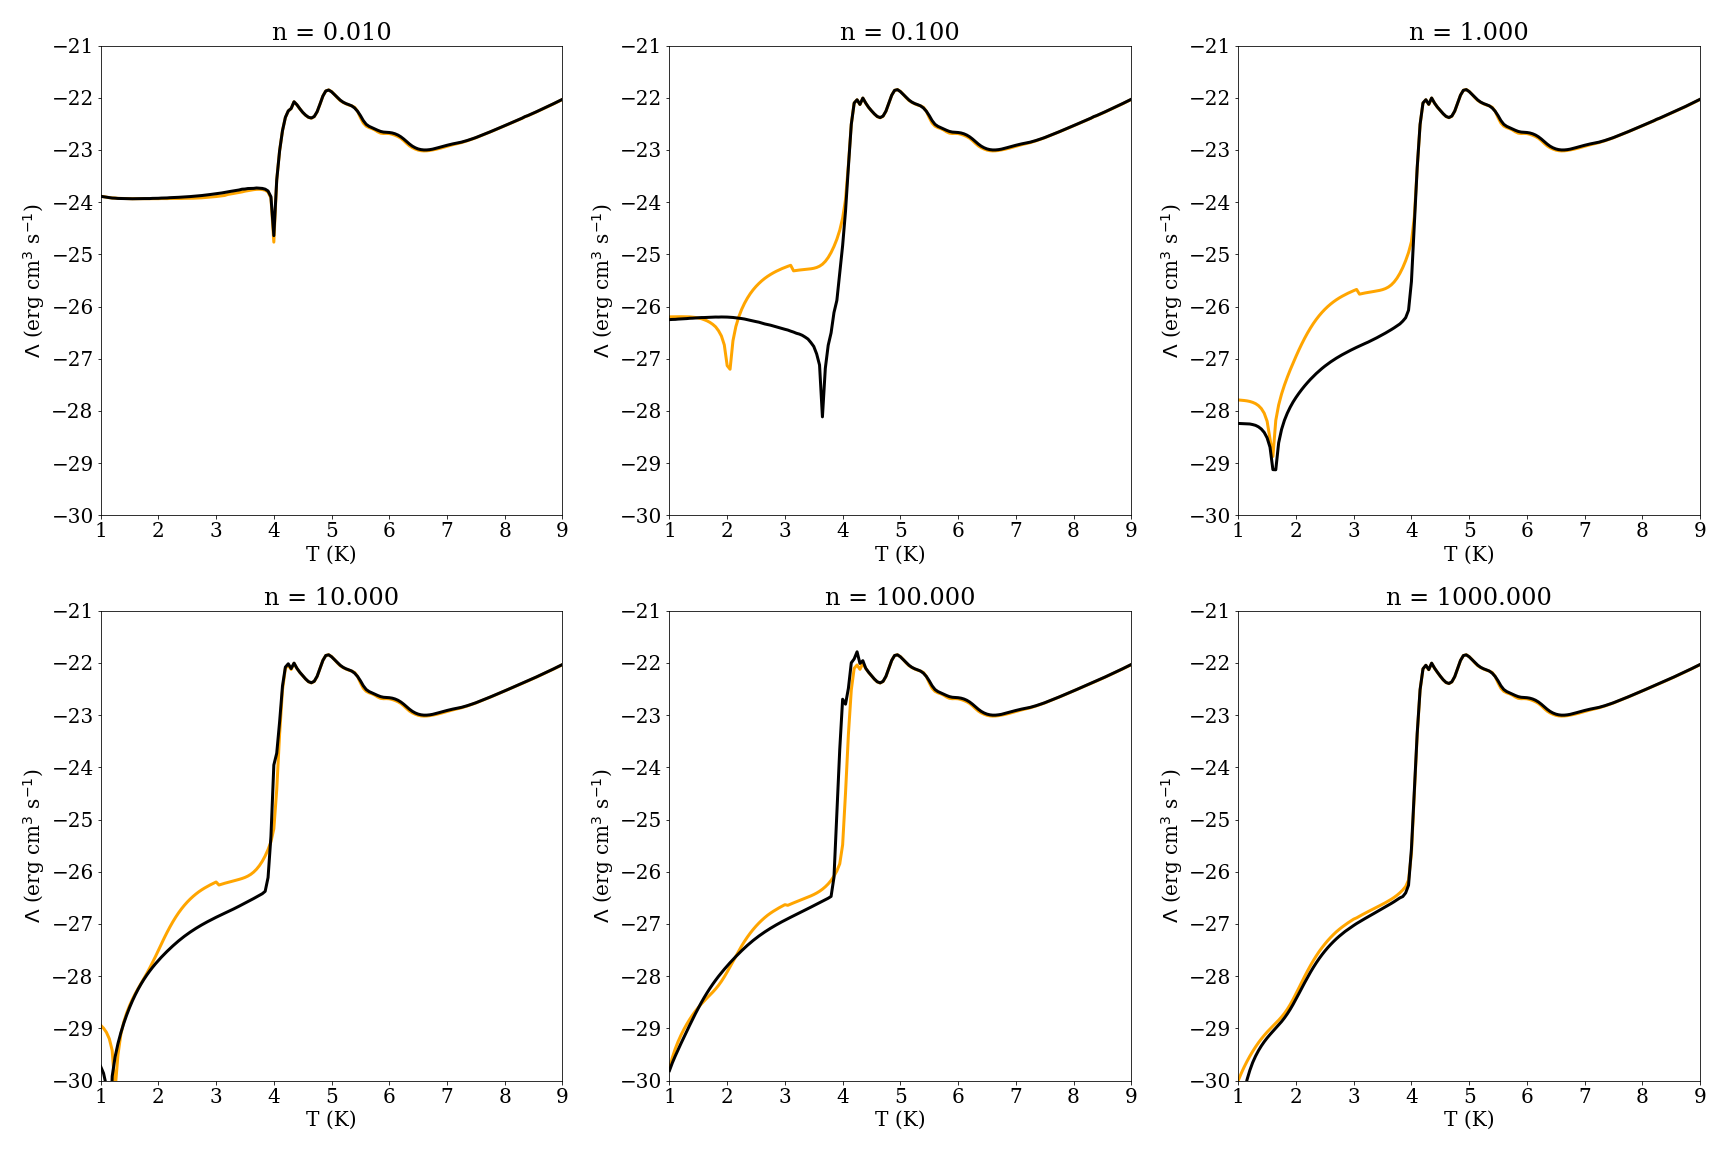
\includegraphics[width=0.95\linewidth]{cooling_model_comparison}
\caption{The absolute value of the net cooling or heating rate 
%mm (|cooling - heating|)
 in two models that account for self-shielding of primordial gas against a metagalactic UV background. Our model (black) uses self-consistent metal line cooling rates, and is compared to an incorrect model (orange) that adopts the un-corrected (i.e. optically thin) metal line cooling rates. The regimes where heating dominates are plotted with dashed lines for clarity.}
\label{fig:cooling comparison}
\end{figure}

\section{Resolution Study}
\label{appendix:resolution study}
We demonstrate the effect of varying resolution on three different results in the evolution of our galaxy model in Figure~\ref{fig:resolution_study}, comparing the star formation rate (left), mass evolution (middle), and metal ejection/retention fractions (right) for our high resolution simulations (solid) as compared to two runs at 3.6 pc with different initial SN driving rates, and a final run at 7.2 pc. The physics in each of these simulations remains the same. However, our star formation algorithm is tied to resolution, since star formation proceeds in gas at densities where the Jeans mass becomes unresolved at the maximum resolution. A factor of two decrease in resolution translates to a factor of four decrease in the star formation density threshold, from 200~cm$^{-3}$ in our fiducial runs, to 50~cm$^{-3}$ and 12.5~cm$^{-3}$ in our 3.6~pc and 7.2~pc resolution runs respectively. 

\begin{figure*}
\centering
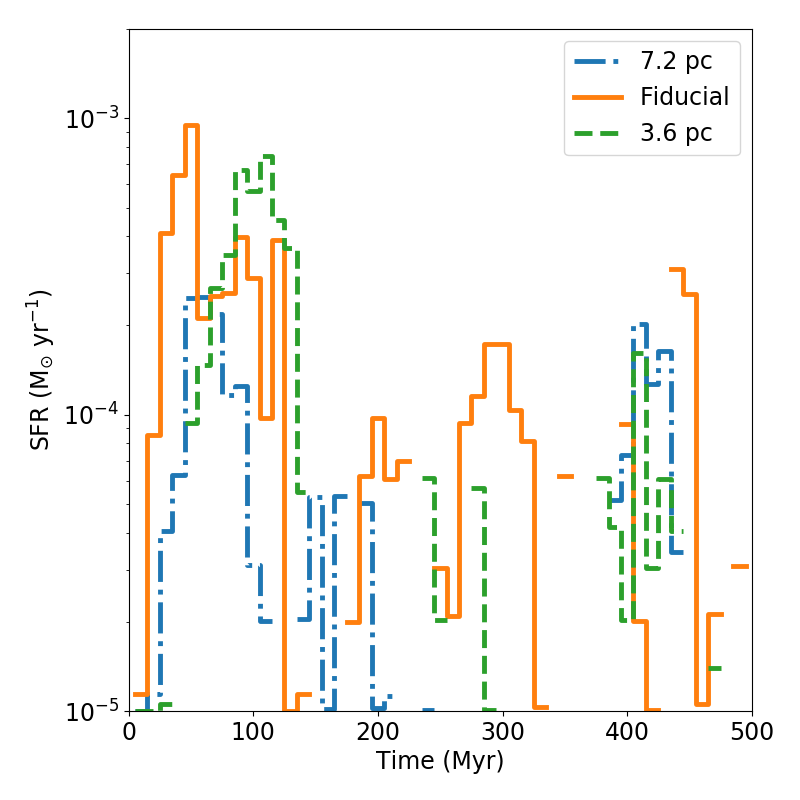
\includegraphics[width=0.33\linewidth]{sfr_resolution_study.png}
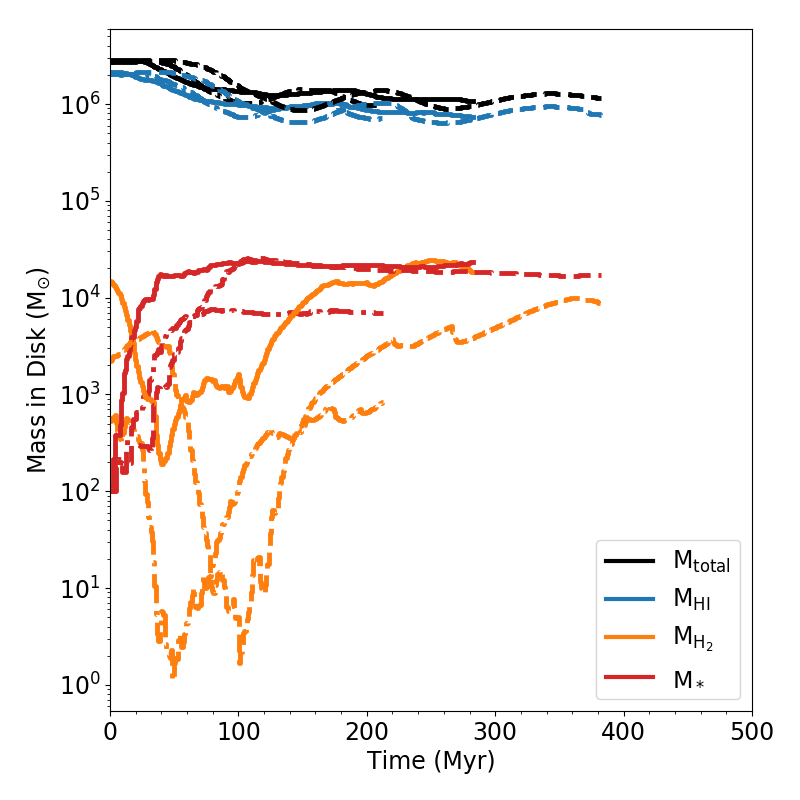
\includegraphics[width=0.33\linewidth]{mass_evolution_resolution.png}
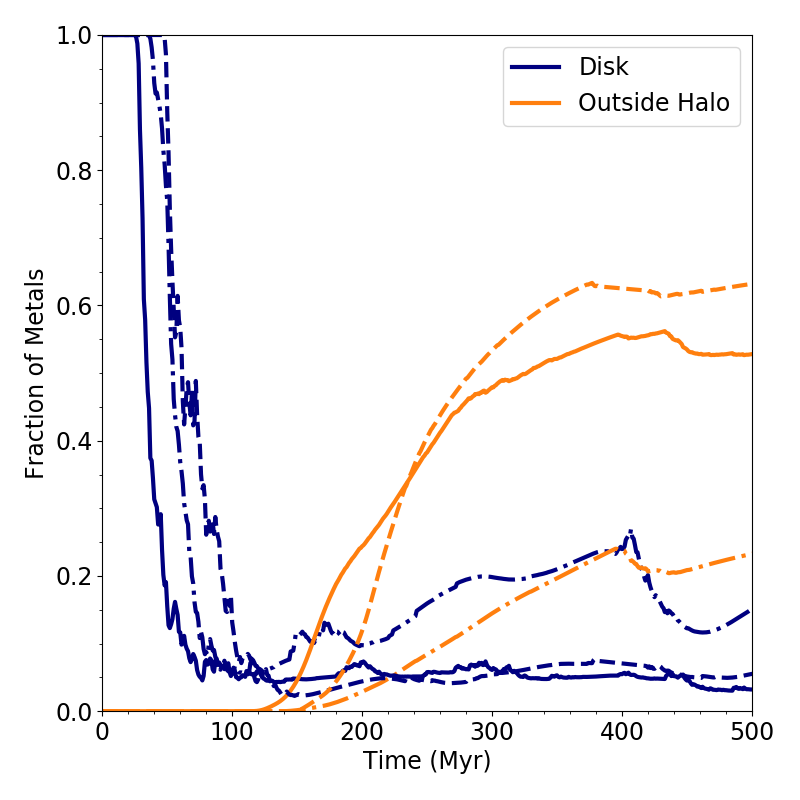
\includegraphics[width=0.33\linewidth]{metal_retention_resolution.png}
\caption{A comparison of the SFR (left), disk gas mass (middle), and metal retention (right) evolution for our fiducial run (solid), 3.6~pc run (dotted), and 7.2~pc run (dash-dotted). We also include a 3.6~pc run with an initial SN driving rate increased by a factor of 2 (dashed). The line colors in the middle panel are the same as in Figure~\ref{fig:sfr_mass_evolution}, where the total disk mass is shown in black, cold gas mass in blue, H$_2$ mass in orange, and stellar mass in red.}
\label{fig:resolution}
\end{figure*}

As shown in these diagrams, resolution certainly changes the evolution, but not dramatically. We argue that these differences are within the stochastic variation one would expect from simulations with stochastic star formation, but point has not been confirmed. Clearly, the initial SFR over the first 100~Myr is different in each simulation; it is larger in each of the lower resolution runs. This is because the initial SN driving is less resolved, leading to over cooling and an increase in the initial star formation rate. This is much less an issue for the SN from real star particles as the pre-SN feedback (winds and radiation) are capable of decreasing the local density enough to resolve the Sedov radius. To test this, we re-ran the 3.6~pc run with an increase in the initial SN driving rate by a factor of 2, which subsequently lowers the initial SFR.

The largest qualitative difference between these runs is the H$_2$ mass. As discussed in this work, the H$_2$ mass fraction of our fiducial run is quite high, driven by significant H$_2$ production from gas-phase reactions and the preferential retention of cold, dense H$_2$ gas in feedback driven outflows. However, each of the lower resolution runs produce less H$_2$ (about 40\% less) than our fiducial run. This is certainly an issue in interpreting the generality of our H$_2$ mass fractions in our fiducial run, and requires more tests to confirm. However, it is not unreasonable to expect that the H$_2$ production occurs most effectively at densities not captured in the 3.6~pc and 7.2~pc runs. This suggests that most of our H$_2$ production in the fiducial run occurs in gas with densities above 50~cm$^{-3}$. To clarify the gas phase differences between these simulations, we present the temperature-density phase diagrams for our 3.6~pc (left) and 7.2~pc (right) simulations in Figure~\ref{fig:phase_resolution} over the same time interval as that presented for our fiducial run in Figure~\ref{fig:phase}. 

\begin{figure*}
\centering
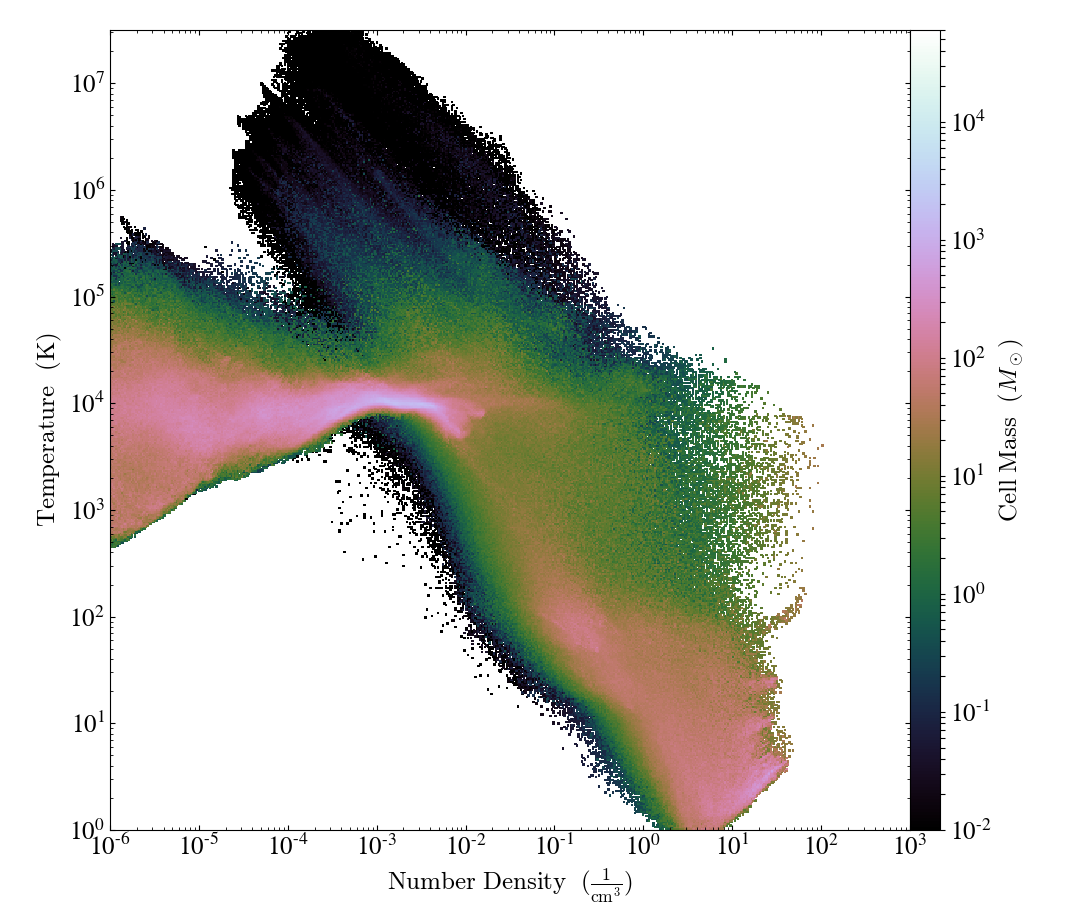
\includegraphics[width=0.475\linewidth]{3pc_phase.png}
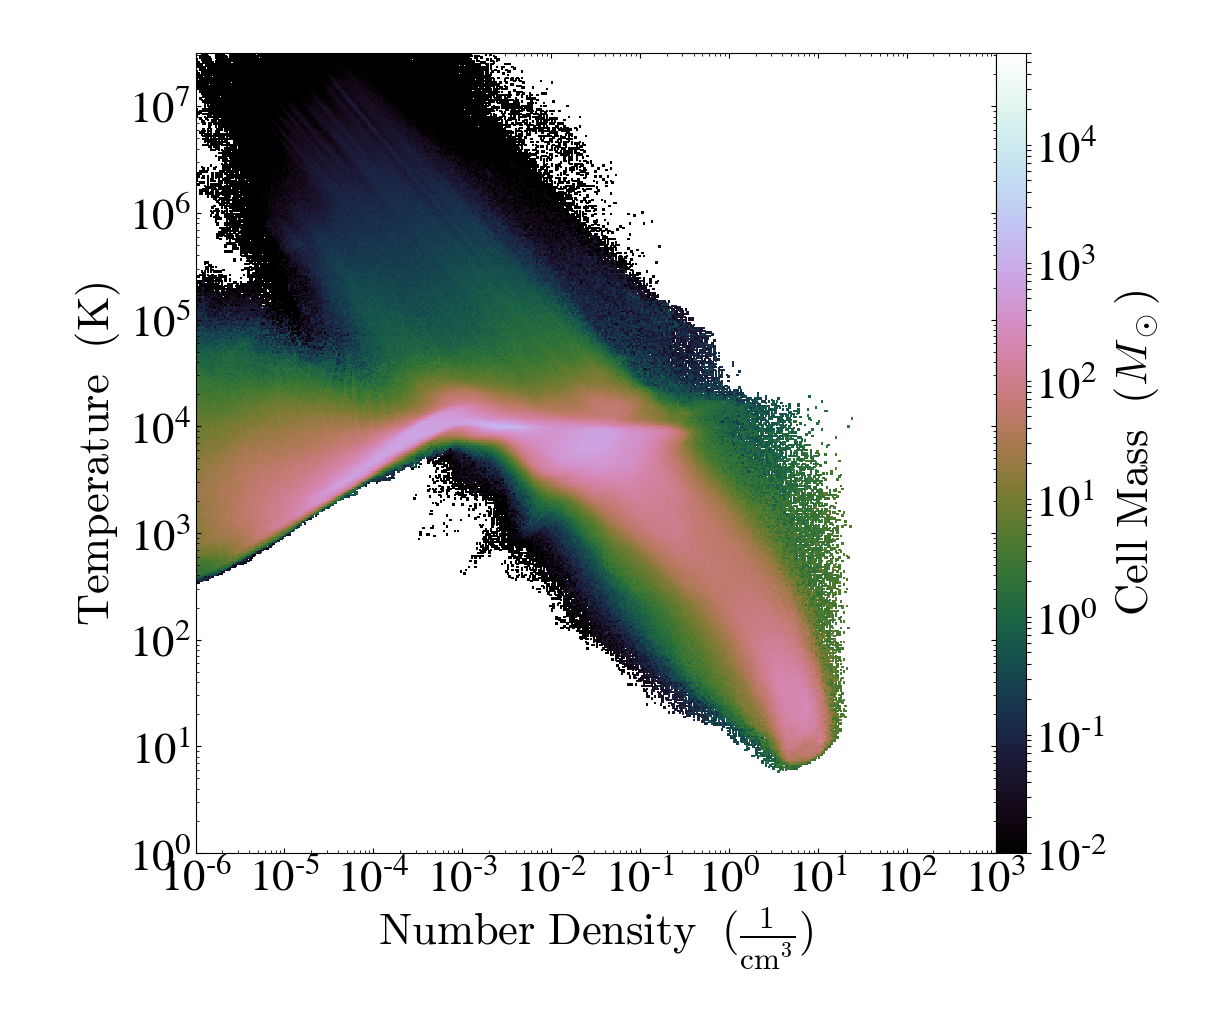
\includegraphics[width=0.475\linewidth]{6pc_phase.png}
\caption{Temperature-density phase diagrams for our 3.6~pc run (left) and 7.2~pc run (right), as presented for our fiducial run in Figure~\ref{fig:phase}.}
\label{fig:phase_resolution}
\end{figure*}

Finally, each of the lower resolution runs retain a surprisingly similar fractions of their produced metals in their disks (black curves in right panel of Figure~\ref{fig:resolution}), but this is about a factor of 2 below what is found in the fiducial run (5\% vs. 10\%). The amount that escapes the halo is significantly more, however. This is an interesting difference, as the resolution decrease primarily affects the disk of the galaxy; little to none of the halo volume is refined to the highest resolution, and so should be unaffected by this change. \textbf{I'm a bit puzzled by this difference...}

%\section{Pre-SN Feedback with and without radiation}

%\section{Code}
%(likely just do this as a short blurb in acknowledgements)

%A one-zone chemical evolution and feedback model was constructed to provide rapid testing and examination of the feedback and yield properties of each of our stars in our model. This code is publically available at https://github.com/aemerick/onez. In the simplest case, one can generate a series of star particles and examine their resulting properties, including wind and supernova yields, as a function of mass and metallicity. Included also are more complicated examples of running the full one-zone model. Support currently only exists for running in a non-cosmological mode with a constant star formation rate. In addition, this one-zone model uses star-by-star modelling and becomes extremely inefficient at large particle counts. Future develop will better optimize this code, allow for variable input or evolving star formation rates, cosmological evolution, and parallelism. 






%\appendix
%\section{appendix section}

\end{document}
